\documentclass{psi-note}    % Specifies the document style.
\usepackage{graphicx}
\usepackage{url}
\usepackage[colorlinks,linkcolor=blue,anchorcolor=blue,citecolor=blue]{hyperref} % hyper reference to contents
\usepackage{algorithm,algorithmic}
\usepackage{tikz}
\usepackage{suffix}
\usetikzlibrary{arrows,shapes,snakes}

\usepackage{draftwatermark}
\SetWatermarkLightness{0.8}
\SetWatermarkScale{4}

\bibliographystyle{apsrev}

\newcommand{\opal}{\textsc{OPAL}}
\newcommand{\opalt}{\textsc{OPAL-t }}
\newcommand{\opalcycl}{\textsc{OPAL-cycl}}
\newcommand{\opalmap}{\textsc{OPAL-map }}
\newcommand{\opalenv}{\textsc{OPAL-envelop}}

\newcommand{\mad}{\textsc{mad }}
\newcommand{\madnine}{\textsc{mad9 }}
\newcommand{\madninep}{\textsc{mad9p }}
\newcommand{\madeight}{\textsc{mad8 }}

\newcommand{\classic}{\textsc{classic }}
\newcommand{\hfifepart}{\textsc{H5Part }}
\newcommand{\hfifefe}{\textsc{H5FED }}

\renewcommand{\epsilon}{\varepsilon} 
\renewcommand{\vec}[1]{{\bf #1}} 
\newcommand{\dt}[1]{\frac{\partial #1}{\partial t}}
\newcommand{\dtt}[1]{\frac{\partial^2 #1}{\partial t^2}}
\newcommand{\dtvec}[1]{\frac{\partial {\mathbf #1}}{\partial t}}
\newcommand{\dttvec}[1]{\frac{\partial^2 {\mathbf #1}}{\partial t^2}}
\newcommand{\rot}{\vec{\nabla} \wedge }
\renewcommand{\div}{\vec{\nabla} \cdot }

\def\vec#1{\mathbf{#1}}
\def\vecg#1{\boldsymbol{#1}}
\def\norm#1{\| #1 \|} 
\def\tr{^{\!\top}}

\def\curl{{\bf curl}\,}
\def\curlp{{\rm curl}_p\,}
\def\div{{\rm div}\,}
\def\grad{\nabla}
\def\gradp{\nabla_p}
\def\dotp#1#2{\langle#1,#2\rangle}
\def\eps{\varepsilon}

\newcommand{\mat}[1]{\ensuremath{\boldsymbol{#1}}}
\newcommand{\vect}[1]{\ensuremath{\mathbf{#1}}}
\newcommand{\iprod}[2]{\ensuremath{\langle#1,#2\rangle}}
\newcommand{\abs}[1]{\ensuremath{|#1|}}

\newcommand{\Nedelec}{N\'{e}d\'{e}lec}

\newcommand{\id}[1]{\structure{#1}}

\newcommand {\Co}{{\mathbb{C}}}
\newcommand {\Int}{{\mathbb{Z}}}
\newcommand {\Nat}{{\mathbb{N}}}
%
%
\newcommand {\Hcurl}{{H(\mathbf{curl};\Omega)}}
\newcommand {\Hocurl}{{H_0(\mathbf{curl};\Omega)}}
\newcommand {\Hdiv}{{H(\mathrm{div};\Omega)}}
\newcommand {\Hodiv}{{H_0(\mathbf{div};\Omega)}}
%
\renewcommand {\Re}{{\rm I \kern-2pt R}}
\newcommand{\vc}[1]{\mbox{\boldmath $#1$}}
\newcommand {\RM}[1]{\mathrm{#1}}



\newcommand{\unit}[2]{$#1\, \rm{#2}$}

\begin{document}           % End of preamble and beginning of text.
 
%%%%%%%%%%%%%%%%%%%%%%%%%%%% PSI-FEL/LEG Title Page %%%%%%%%%%%%%%%%%%%%%%%%%%%%%%%%%
\feltitle{
  PSI-TMxx-xxx-xx
}{
  IMPACT-T, Astra \& \opal\ Code Comparison
}{
  A. Adelmann, Y. Ineichen, Ch. Kraus,  \\ A. Oppelt (DESY), S. Russel (LANL) and  C. Gulliford (Cornell)
}{
  \PSI
}{
  \felabstract{
    In this note we compare IMPACT-T, Astra and \opal\ in the SwissFEL context.
  }
}
%%%%%%%%%%%%%%%%%%%%%%%%%%%%%%%%%%%%%%%%%%%%%%%%%%%%%%%%%%%%%%%%%%%%%%%%%%%%%
\section{Introduction}

In section \ref{sec:OPALAstra} we compare Astra and \opalt using a setup
with a CTF3 gun \cite{CTF3Gun} followed by two S-Band traveling wave (tw)
structures and a total of nine solenoids. The gun is at a nominal phase of $-3.5$~degree and has a
accelerating gradient of $100$~MV/m. Both tw structures are operated on crest. They have
accelerating gradients of $19$~MV/m and $22$~MV/m respectively. First (in \ref{sec:OPALAstra-noSC}) we show the case without space charge ($I=0$), followed by
the nominal case of $Q=200$~pC.


In section \ref{sec:tt-vs-et} we compare \opalt\ and \opale on the problem of section \ref{sec:OPALAstra}.

In section \ref{sec:OPALImpactt} we compare IMPACT-T and \opalt with two
separate tests:\\ 
The first test in section \ref{sec:Drift} reads in a particle distribution and
tracks the particles in free space until they enter a solenoid magnet. Full 3D
space charge calculations are enabled.

The second test presented in section \ref{sec:Gun} consists of a $500~\mbox{kV}$ 
pulser followed by a solenoid magnet system. The field solver must deal with
many (39) Lorentz frames in order to correctly model the large energy spread in
the long electron pulse.

The parallel performance is evaluated by comparing the time
to solution only, for a SwissFEL related computation (section
\ref{sec:OPALAstra}). More details on performance of \opal\ can be found in
\cite{PhysRevSTAB.13.064201,Adelmann20104554}.

\section{\opal-T \& Astra} \label{sec:OPALAstra}

We simulate a setup based on the PSI $250$~MeV test injector up
to $130$~MeV. The nominal gun phase is at $\phi_g = -3.5$~degrees, both S-Band
structures are on crest.


\subsection{Initial Conditions}

We use the parameters given in table \ref{tab:ic} to specify the initial
condition of the simulation. Some details on the emission model of \opal\ are given
in appendix~\ref{app:emission}. 
\begin{table}[h]\footnotesize
{\renewcommand{\arraystretch}{1.5}
\renewcommand{\tabcolsep}{0.5cm}}
\caption{Initial conditions}
\centering
  \label{tab:ic}
  \begin{tabular}{ l  l   l  }
    \hline
    
    $\sigma_x$  &  $249 $ & $\mu$m \\
    $\sigma_y$  &  $249 $ & $\mu$m \\
    $Q$  &  $200 $ & pC \\
    $t_{\rm fwhm}$  & 9.9 & ps \\
$t_{\rm rise}=t_{\rm fall}$ & 0.782 \footnotemark[1]& ps \\	
$E_{\rm th}$ & 0.65 & eV \\
      \hline 
 \hline
  \end{tabular}
 \end{table}
\footnotetext[1]{we define $t_{\rm rise}$ as the time difference between the moment when the current at the cathode reaches 10~\% of its maximum and the moment when it reaches 90~\%. With this definition we measured in the Astra histogram a rise time of \unit{0.782}{ps} when we specified \unit{0.7}{ps} in the input file.}
\begin{figure}[htbp]
\begin{center}
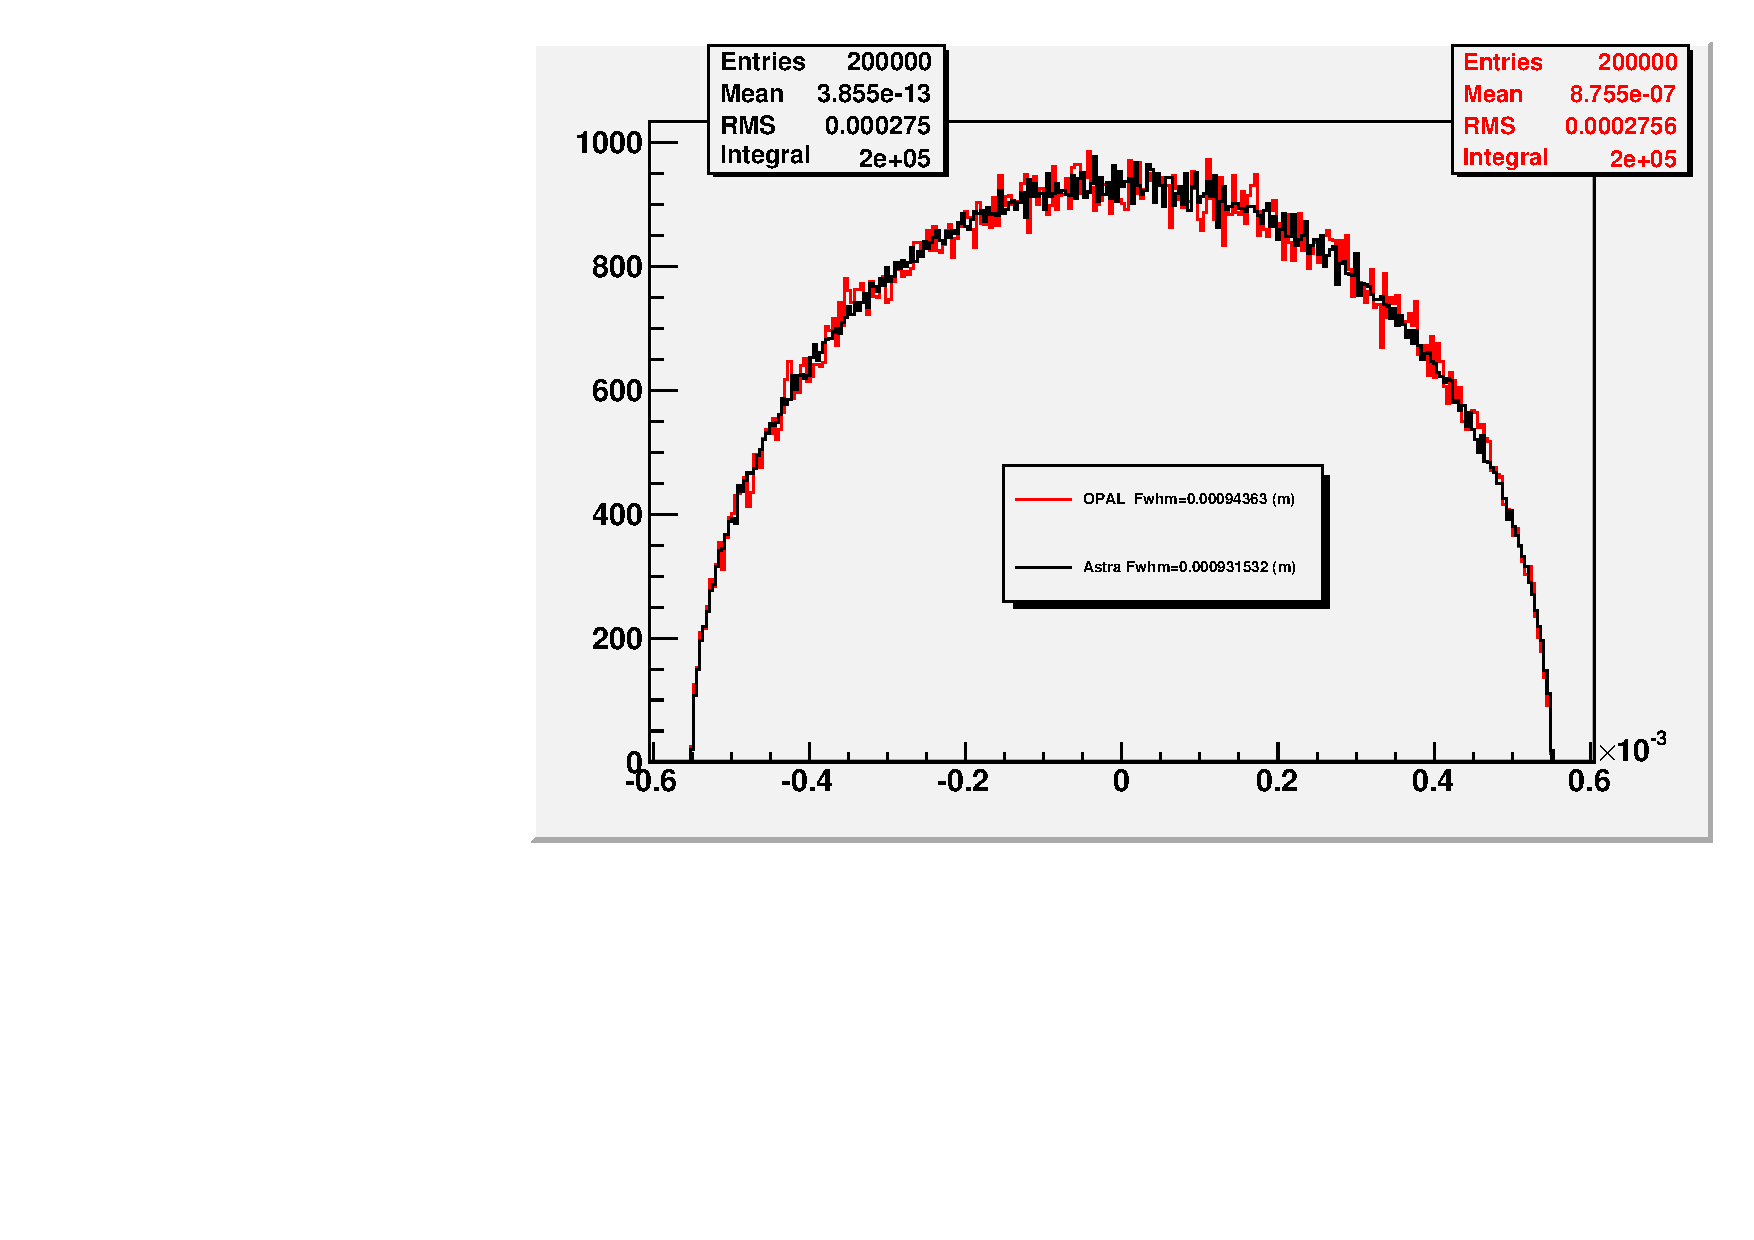
\includegraphics[width=.49\linewidth,angle=0]{figures/opal-astra-x}
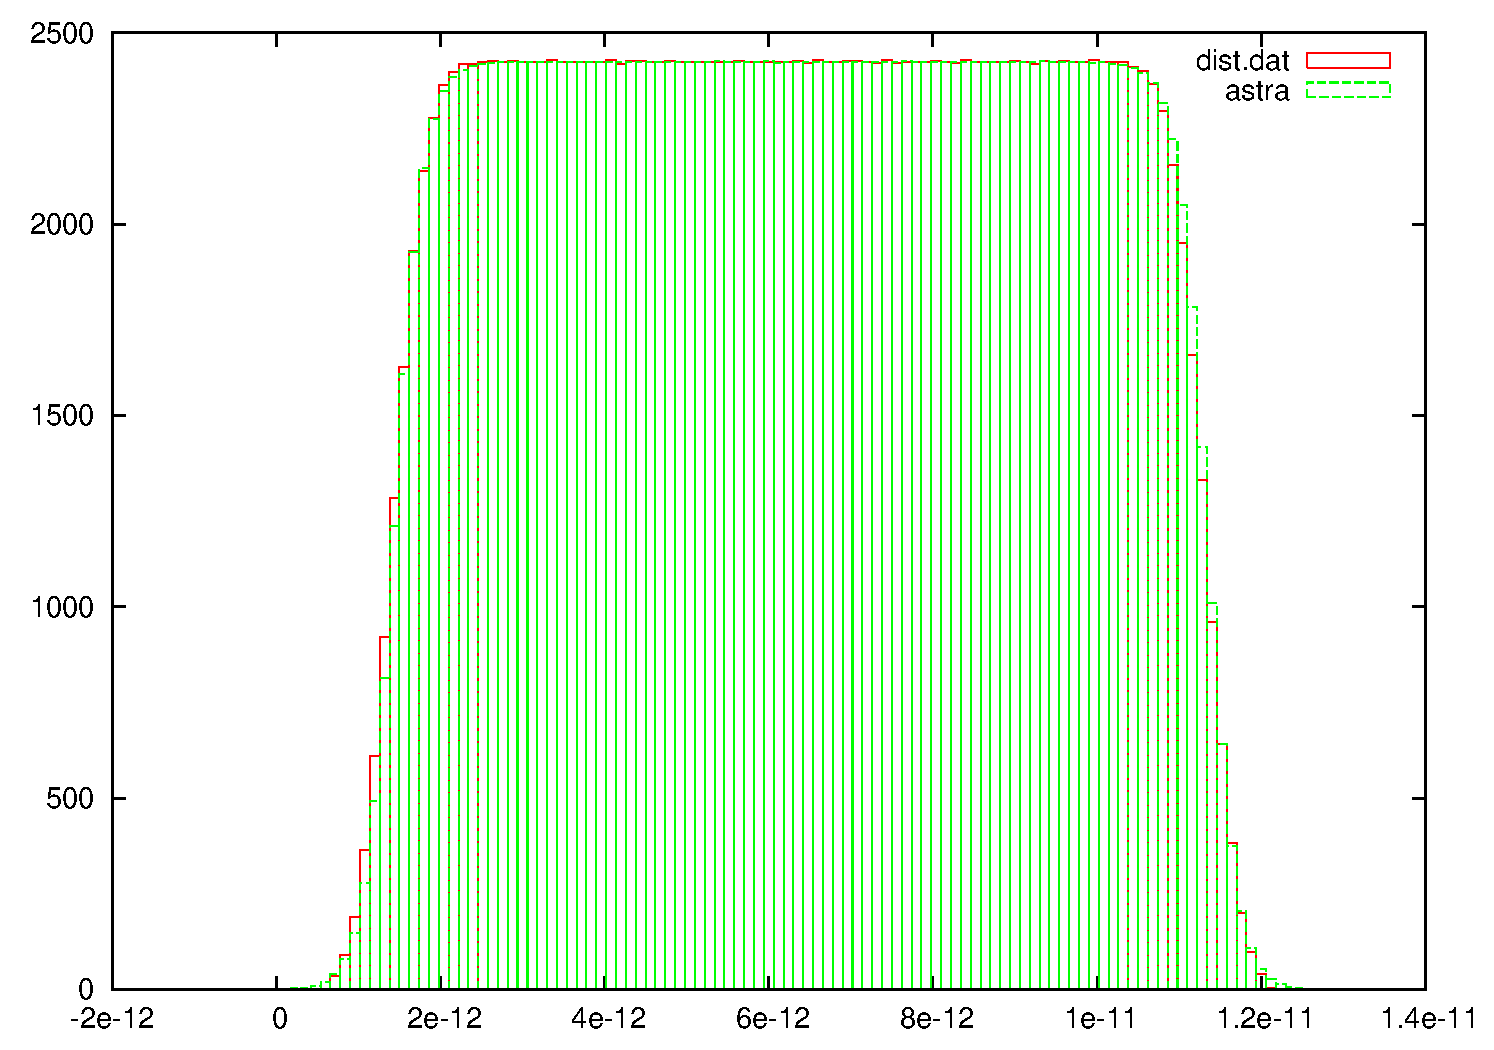
\includegraphics[width=.49\linewidth,angle=0]{figures/opal-astra-t}
\caption{Initial conditions of the spatial $x$ and temporal $t$ variable}
\label{fig:opal-astra-exrms-1}
\end{center}
\end{figure}
To approximate the histogram of the longitudinal distribution of Astra we used a convolution of a rectangular function with width equal to $t_{\rm fwhm}$ and a Gaussian function. The $\sigma$ of the Gaussian function is determined by $t_{\rm rise}$\footnotemark[1]. This leads to small differences at the tails of the distribution.

\subsubsection{Undocumented Astra Switch}

In order to have the Astra data at fixed time steps, make sure {\tt Local\_emit=.F}.

\subsubsection{Autophasing}
The values in the Table \ref{tab:aph} showing the absolute differences when comparing phases and energies 
after autophase has completed. 
\begin{table}[h]\footnotesize
{\renewcommand{\arraystretch}{1.5}
\renewcommand{\tabcolsep}{0.5cm}}
\caption{Initial conditions}
\centering
  \label{tab:aph}
  \begin{tabular}{ l  l   l  }
    \hline
    
    &  d$\phi$ (deg) & dE (keV)  \\
    \hline
    Gun  &  0.059  & 2.85 \\
    First TW Structure  &  0.42 & 6.5 \\
    Second TW Structure & 0.109 & 15 \\

      \hline 
 \hline
  \end{tabular}
 \end{table}


\subsection{Simulations without space charge}  \label{sec:OPALAstra-noSC}
In both codes the space charge is turned off. 
Since the field strengths of the solenoids are adjusted for the case with space charge the beam is overfocused. The emphasis is on the comparison between the two codes and not on modeling a real machine.
Note:
\begin{enumerate}
\item in some plots the agreement is such that the two graphs are hardly distinguishable
\item contrary to Astra in \opalt we do not compensate the rotation in the solenoidal fields.
\end{enumerate}

The final values of important quantities are shown in Table \ref{tab:finalzerocurr} and some graphs of this case are presented in the  Figures \ref{fig:opal-astra-nosc-energy-1}
and \ref{fig:opal-astra-nosc-rmsvals-1}.

\begin{table}[h]\footnotesize
{\renewcommand{\arraystretch}{1.5}
\renewcommand{\tabcolsep}{0.5cm}}
\caption{Final conditions no space charge at $12$m }
\centering
  \label{tab:finalzerocurr}
  \begin{tabular}{ l  l l  l  }
    \hline   
    &    \opal  & Astra  \\
    \hline
    $E_{final}$  &  $130.408$  & $130.380$ & (MeV) \\
    $\Delta E_{final}$  & $90.0992$   &  $83.7400$ & (keV) \\
    $\eps_x$  rms & $0.26797$    &    $ 0.26844$ & (mm-mr)\\
    $x$ rms  & $247.553$    &     $248.870$ & ($\mu$m)\\
    $z$ rms  &  $600.460$ &       $594.250$  & ($\mu$m)\\
      \hline 
 \hline
  \end{tabular}
 \end{table}

\begin{figure}[htbp]
\begin{center}
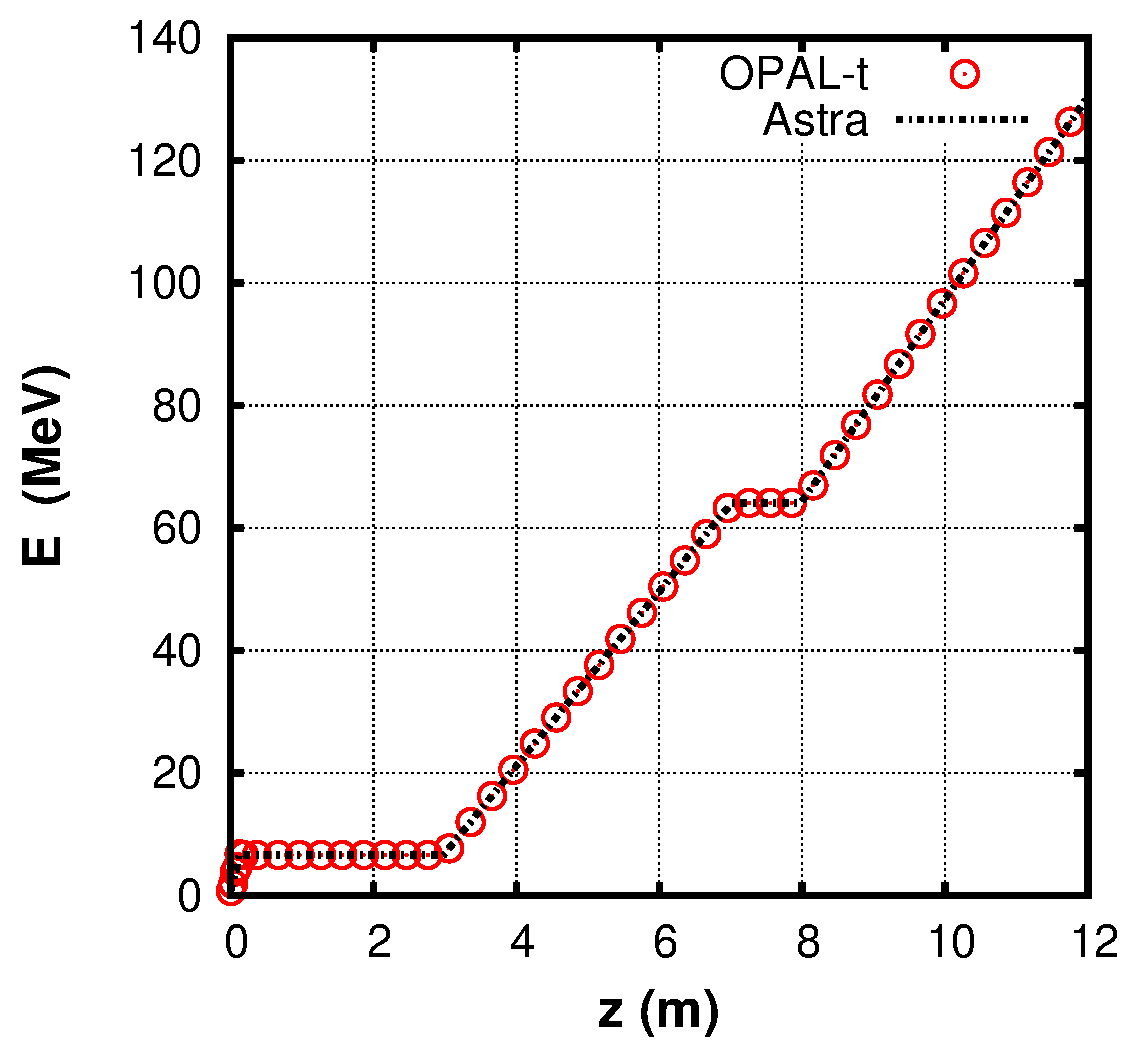
\includegraphics[width=.49\linewidth,angle=0]{figures/opal-astra-nosc-energy-1}
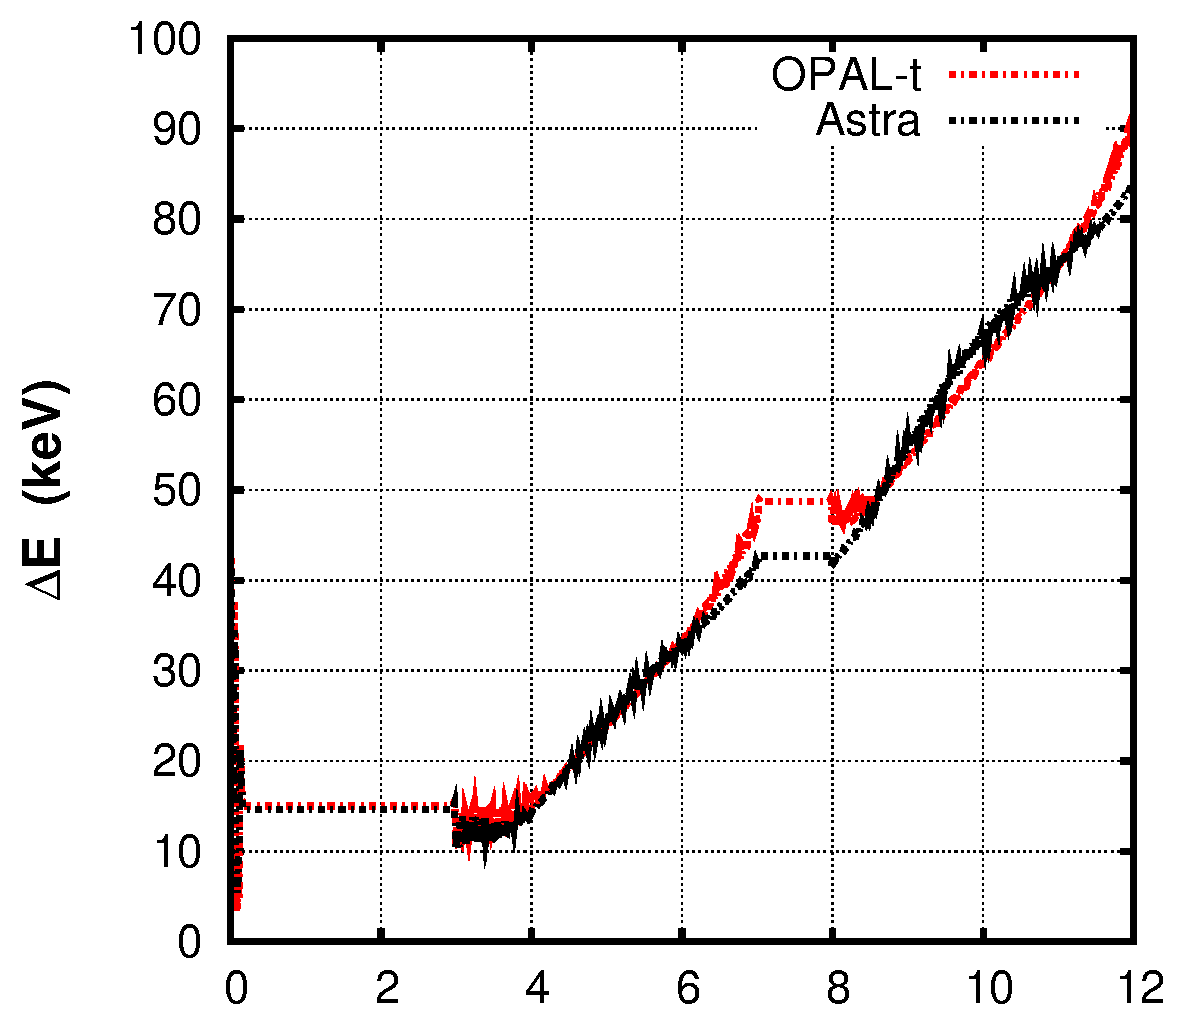
\includegraphics[width=.49\linewidth,angle=0]{figures/opal-astra-nosc-de-1}
\caption{The kinetic energie and the RMS energy spread in the case of $I=0$. }
\label{fig:opal-astra-nosc-energy-1}
\end{center}
\end{figure}

\begin{figure}[htbp]
\begin{center}
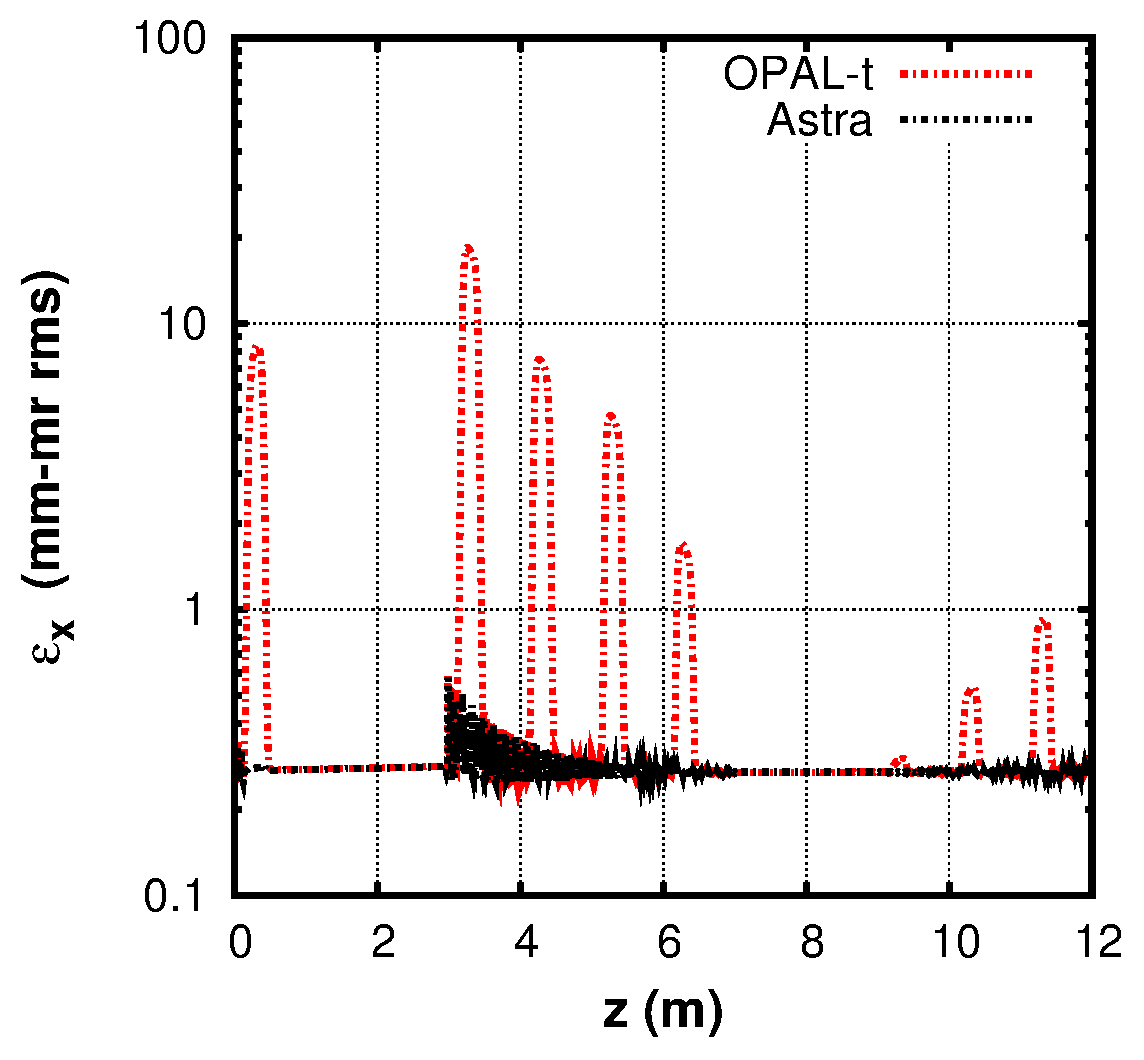
\includegraphics[width=.49\linewidth,angle=0]{figures/opal-astra-nosc-exrms-1}
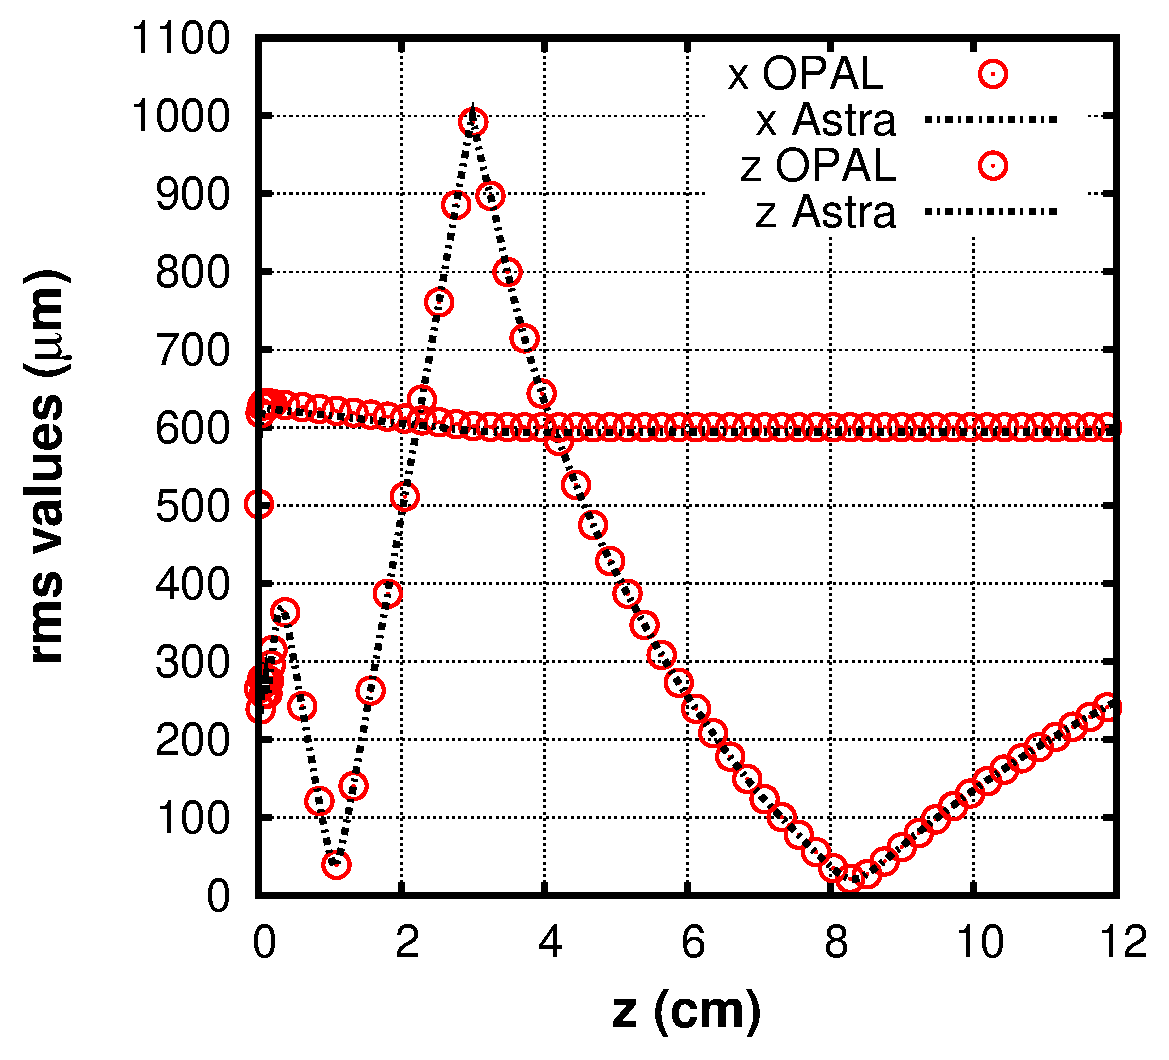
\includegraphics[width=.49\linewidth,angle=0]{figures/opal-astra-nosc-xzrms-1}
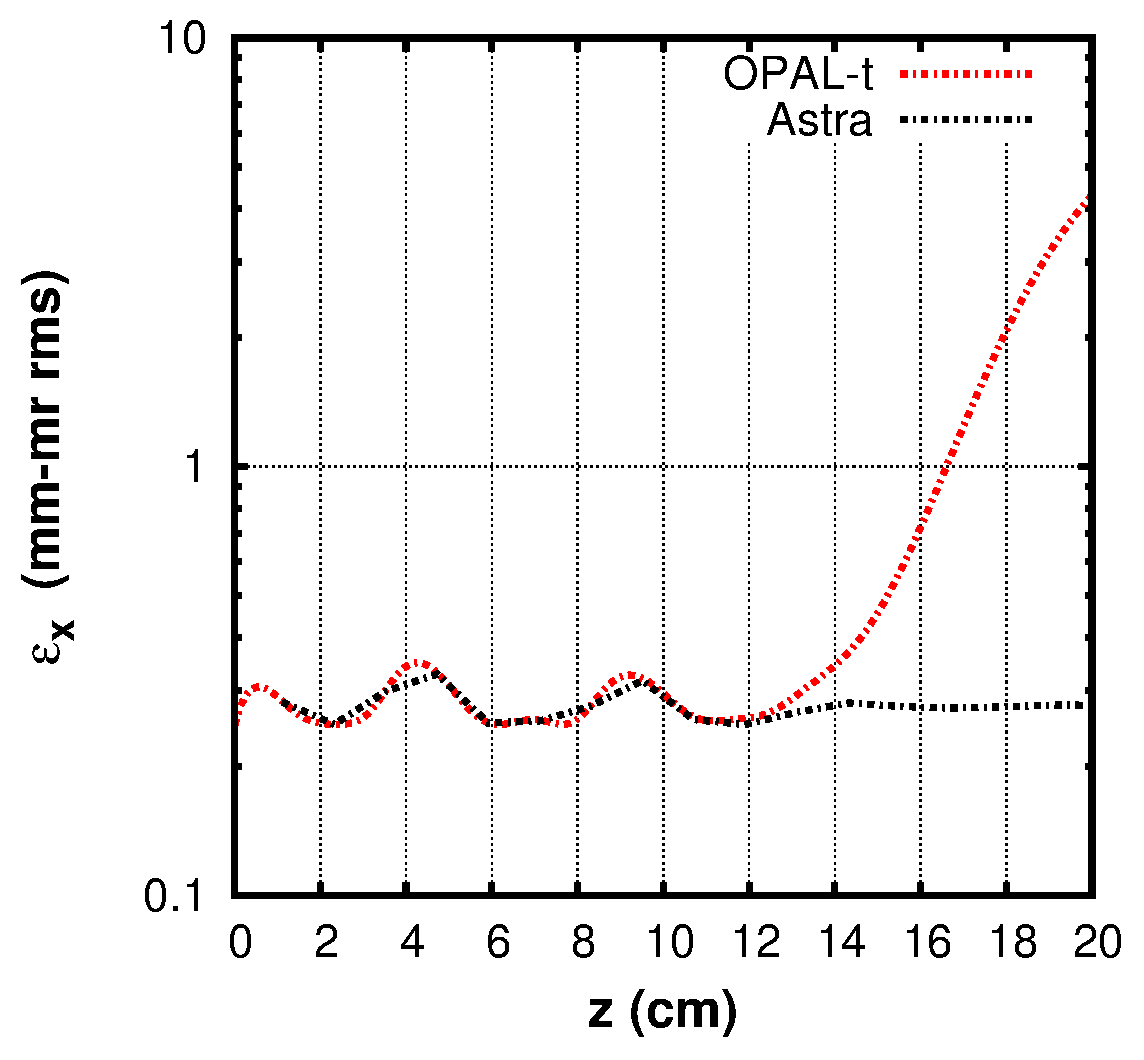
\includegraphics[width=.49\linewidth,angle=0]{figures/opal-astra-nosc-exrms-2}
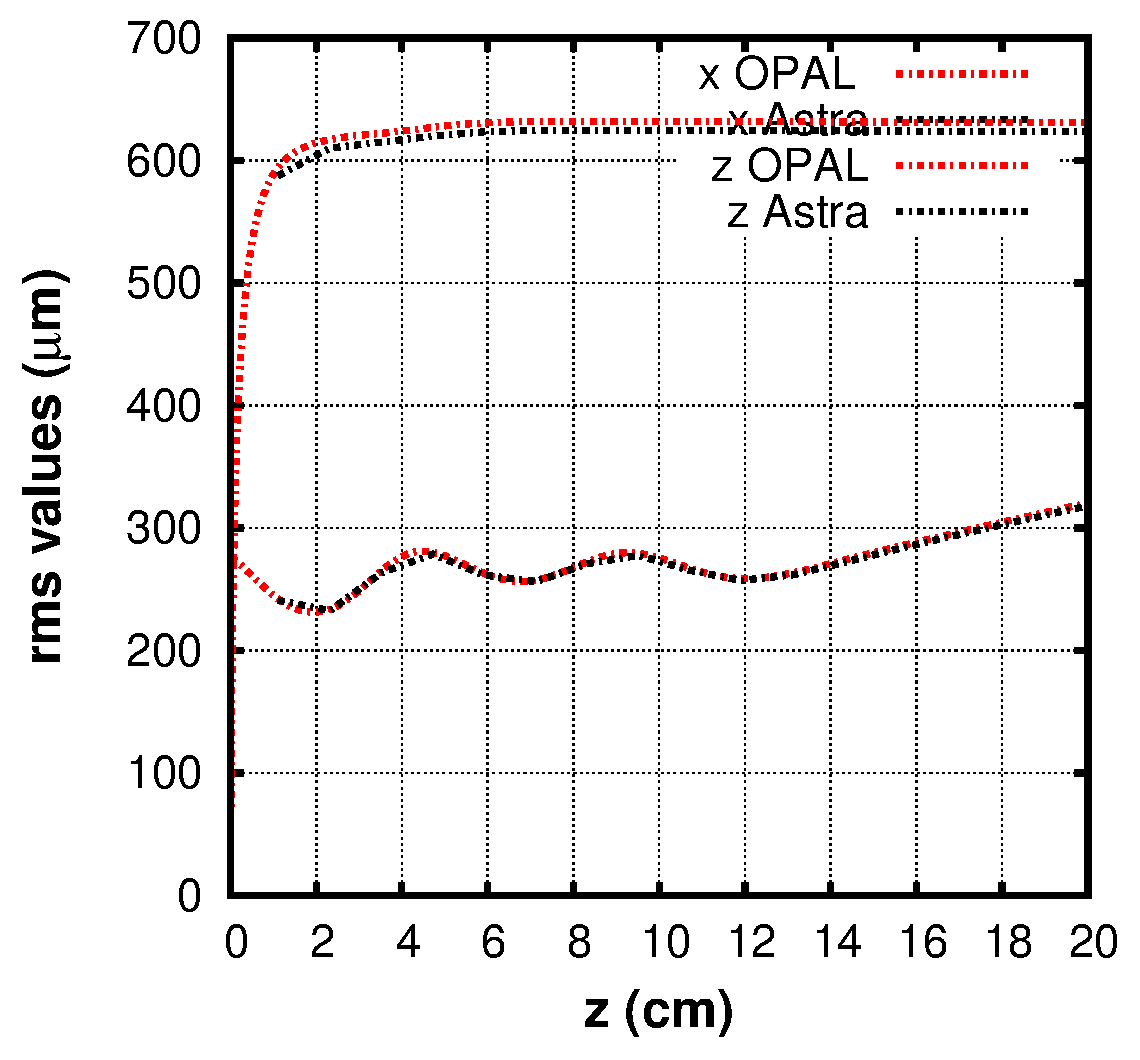
\includegraphics[width=.49\linewidth,angle=0]{figures/opal-astra-nosc-xzrms-2}
\caption{The RMS emittancees (left) and beam sizes (right) in the case of $I=0$. Above is an overview, below is a detail of the first \unit{20}{cm}.}
\label{fig:opal-astra-nosc-rmsvals-1}
\end{center}
\end{figure}
\clearpage

\subsection{Adjusting the Phases}

Adjusting the phase of the gun by 0.5 (nominal phase now -3.0) degree
and the first TWS by 0.1 (nominal phase now 0.1) degrees, the agreement can even further increased as shown in
Table {\ref{tab:finalzerocurrajustph} and Figure \ref{fig:finalzerocurrajustph}. The difference in rms energy spread between the two codes
in now $\sim 3$\% .

\begin{table}[h]\footnotesize
{\renewcommand{\arraystretch}{1.5}
\renewcommand{\tabcolsep}{0.5cm}}
\caption{Final conditions no space charge at $12$m }
\centering
  \label{tab:finalzerocurrajustph}
  \begin{tabular}{ l  l l  l  }
    \hline   
    &    \opal  & Astra  \\
    \hline
    $E_{final}$  &  $130.343$  & $130.380$ & (MeV) \\
    $\Delta E_{final}$  & $86.4020$   &  $83.7400$ & (keV) \\
    $\eps_x$  rms & $0.27063$    &    $ 0.26844$ & (mm-mr)\\
    $x$ rms  & $247.843$    &     $248.870$ & ($\mu$m)\\
    $z$ rms  &  $602.582$ &       $594.250$  & ($\mu$m)\\
      \hline 
 \hline
  \end{tabular}
 \end{table}

\begin{figure}[htbp]
\begin{center}
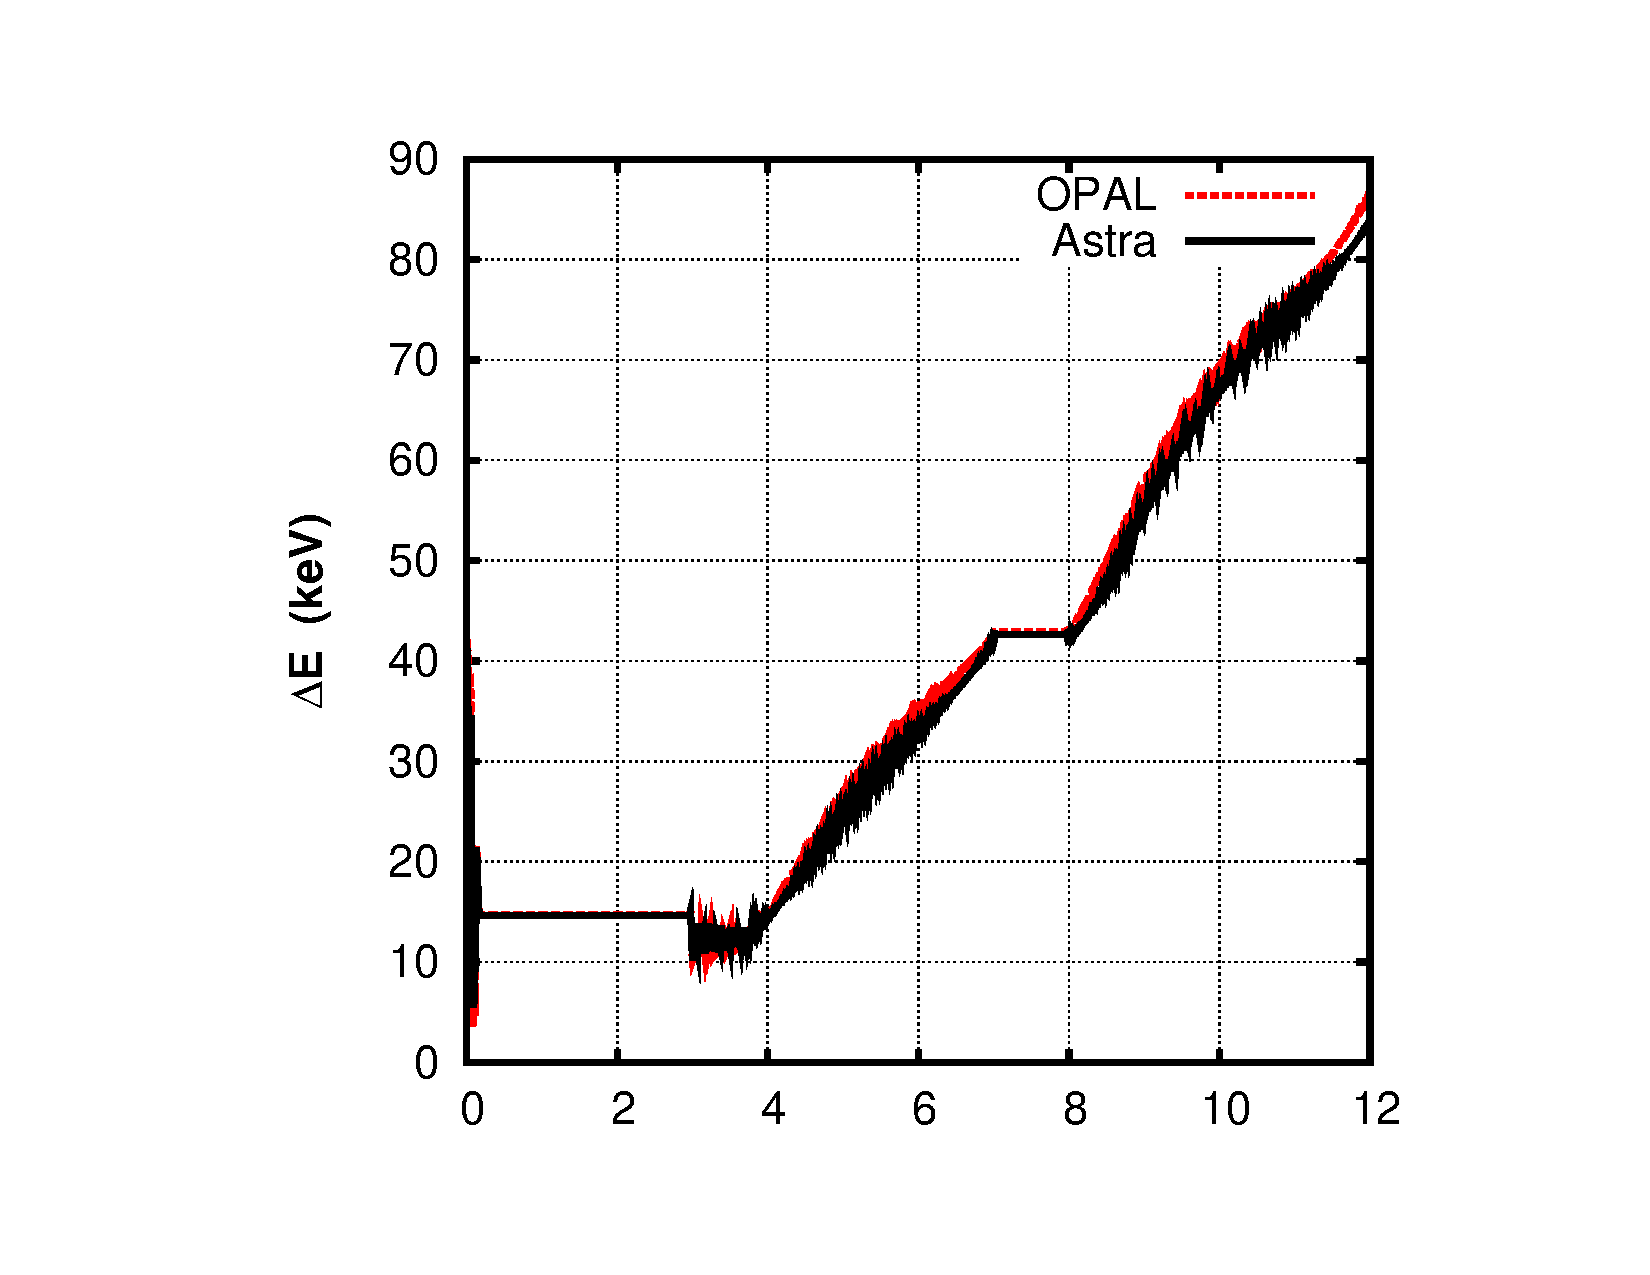
\includegraphics[width=.89\linewidth,angle=0]{figures/opal-astra-nosc-de-3}
\caption{Energy spread after phase adjustment}
\label{fig:finalzerocurrajustph}
\end{center}
\end{figure}

\subsection{Energy profile and energy spread for the $Q=200$~pC case}  \label{sec:OPALAstra-SC}
The final values of important quantities are shown in Table \ref{tab:finalcurr} and some graphs of this case are presented in the  Figures \ref{fig:opal-astra-energy-1}
and \ref{fig:opal-astra-nosc-rmsvals-1}.

\begin{table}[h]\footnotesize
{\renewcommand{\arraystretch}{1.5}
\renewcommand{\tabcolsep}{0.5cm}}
\caption{Final conditions with space charge ($Q=200$~pC) at $12$m }
\centering
  \label{tab:finalcurr}
  \begin{tabular}{ l  l l  l  }
    \hline
    &    \opal  & Astra  \\
    \hline
    $E_{final}$  &  $130.249$  & $130.290$ & (MeV) \\
    $\Delta E_{final}$  & $184.79$   &  $213.22$ & (keV) \\
    $\eps_x$  rms & $0.46990$    &    $ 0.49075$ & (mm-mr)\\
    $x$ rms  & $377.648$    &     $412.510$ & ($\mu$m)\\
    $z$ rms  &  $809.092$ &       $826.860$  & ($\mu$m)\\
      \hline
 \hline
  \end{tabular}
 \end{table}

\begin{figure}[htbp]
\begin{center}
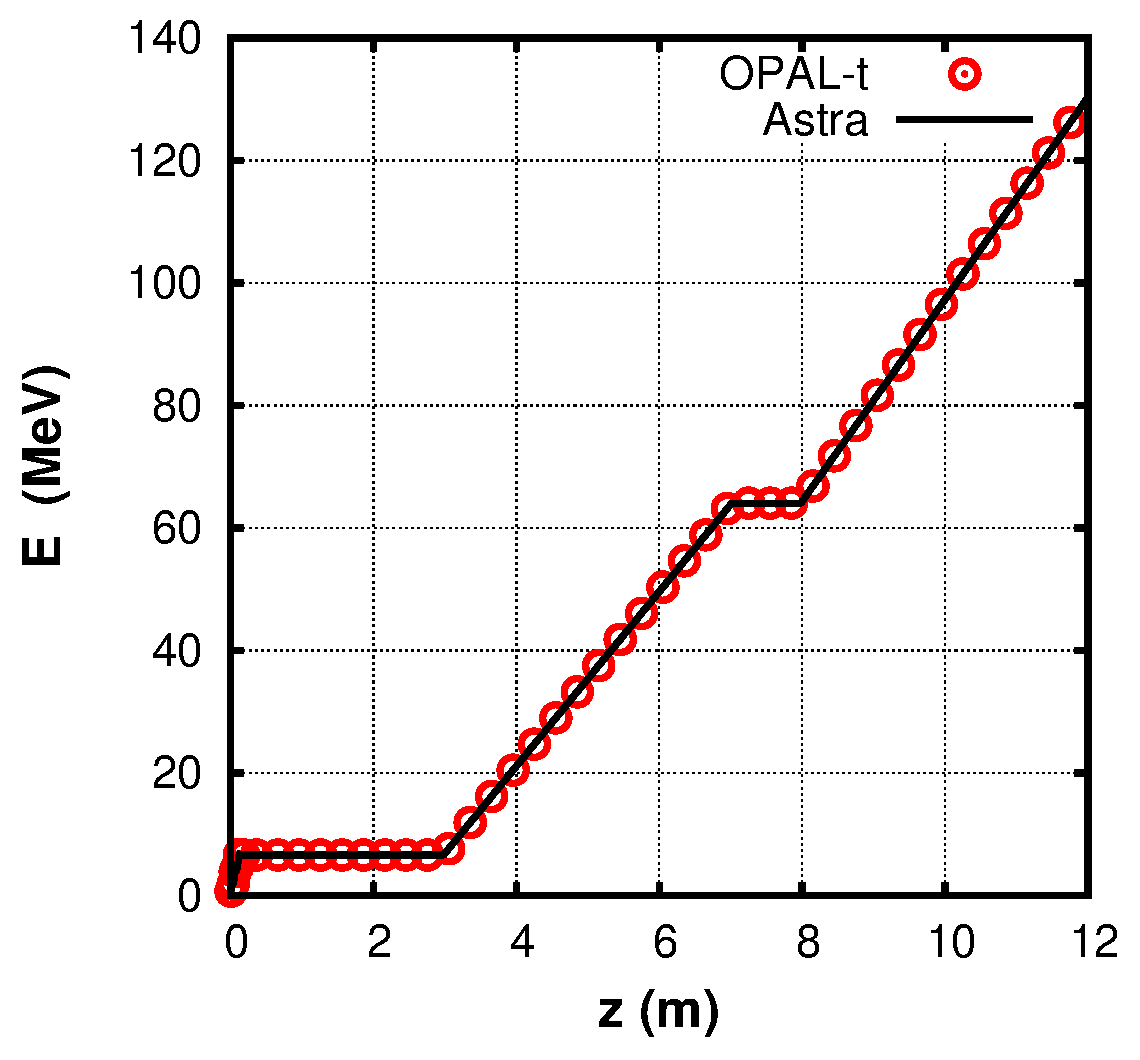
\includegraphics[width=.49\linewidth,angle=0]{figures/opal-astra-sc-energy-1}
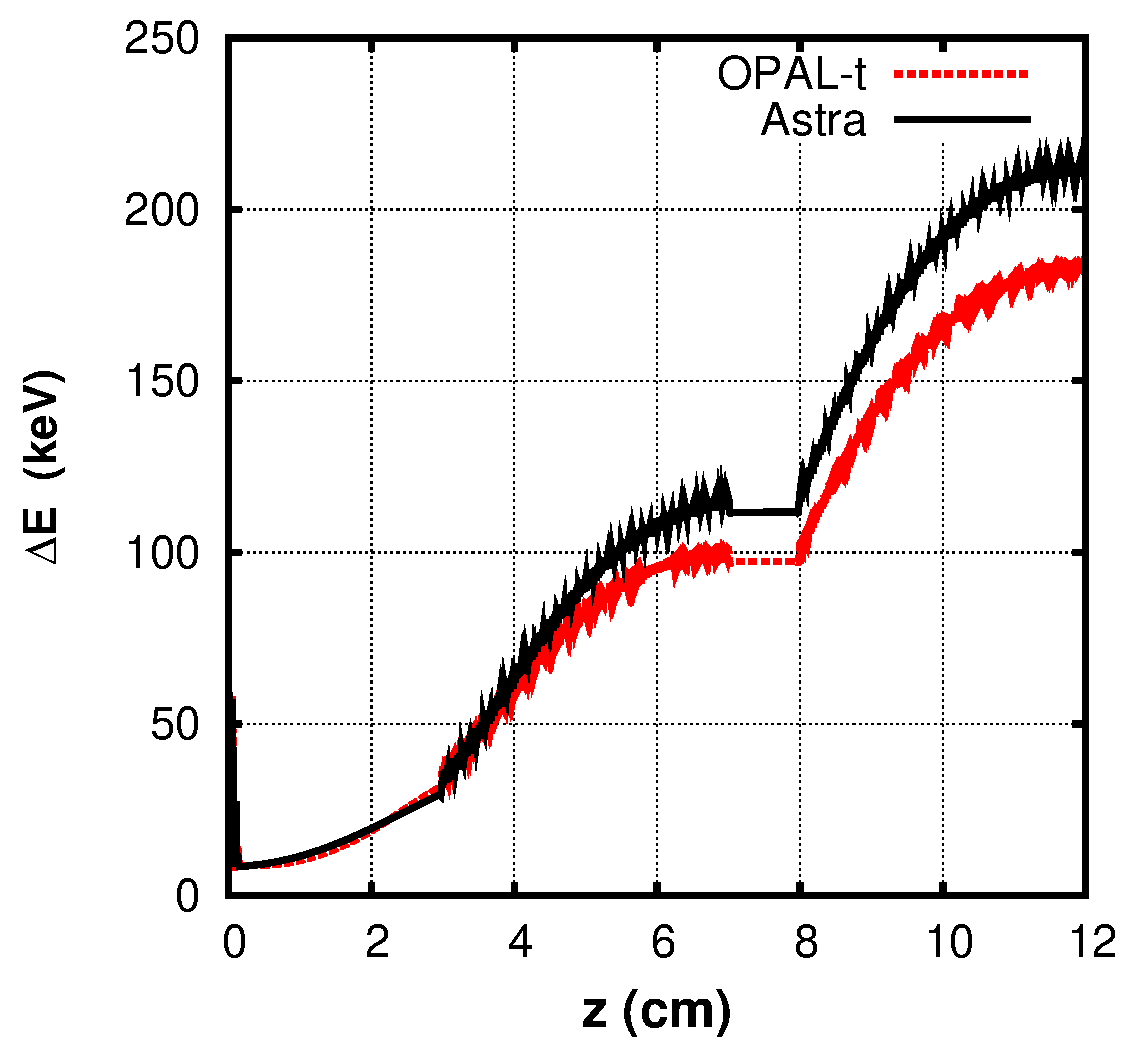
\includegraphics[width=.49\linewidth,angle=0]{figures/opal-astra-sc-de-1}
\caption{The kinetic energies and the RMS energy spread }
\label{fig:opal-astra-energy-1}
\end{center}
\end{figure}
\clearpage
\subsubsection{RMS Beam Sizes (upper left and right)  and Normalized Emittances (lower left and right) }
\begin{figure}[htbp]
\begin{center}
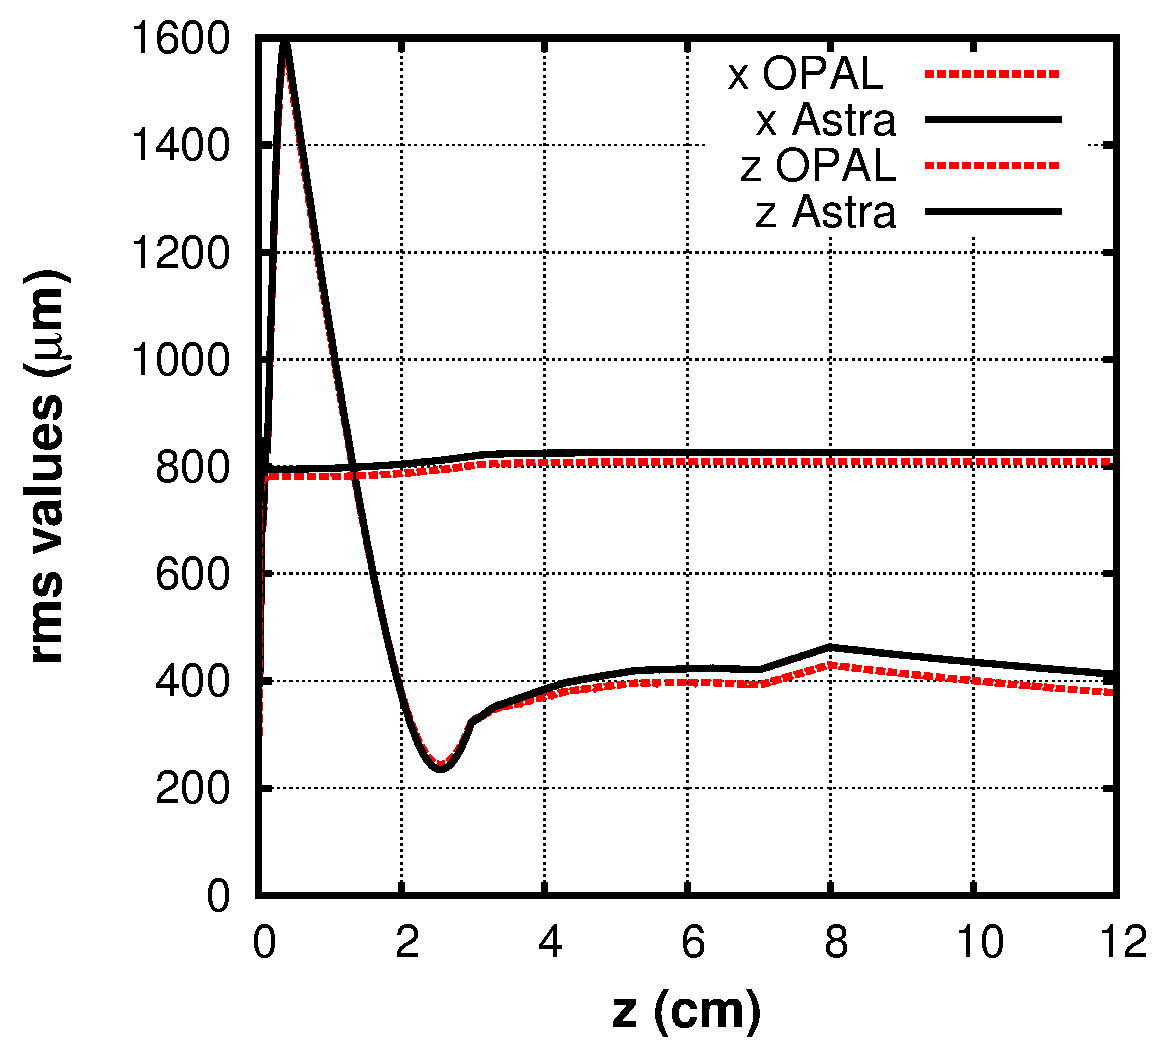
\includegraphics[width=.49\linewidth,angle=0]{figures/opal-astra-sc-xzrms-1}
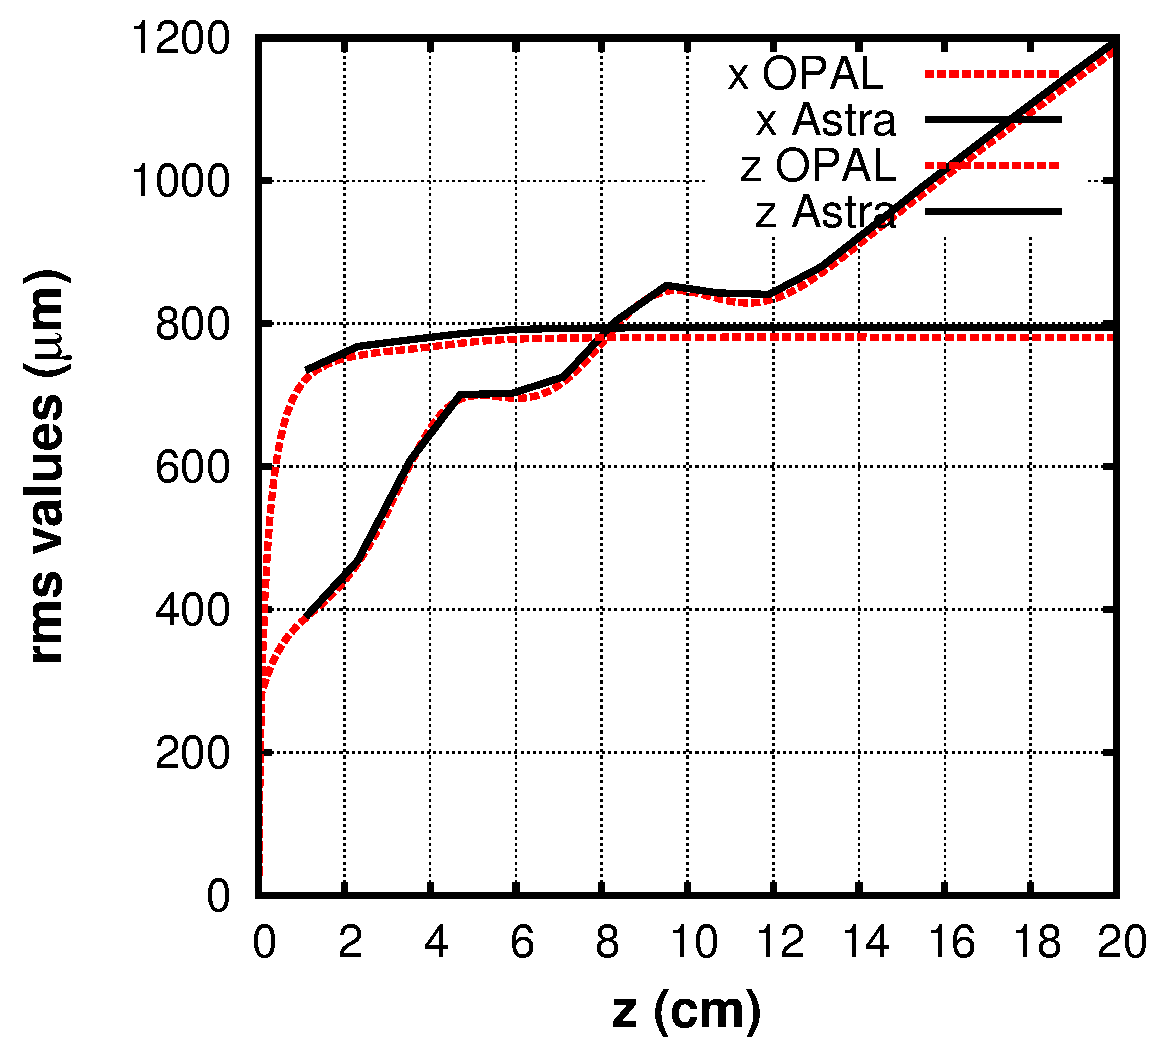
\includegraphics[width=.49\linewidth,angle=0]{figures/opal-astra-sc-xzrms-2}
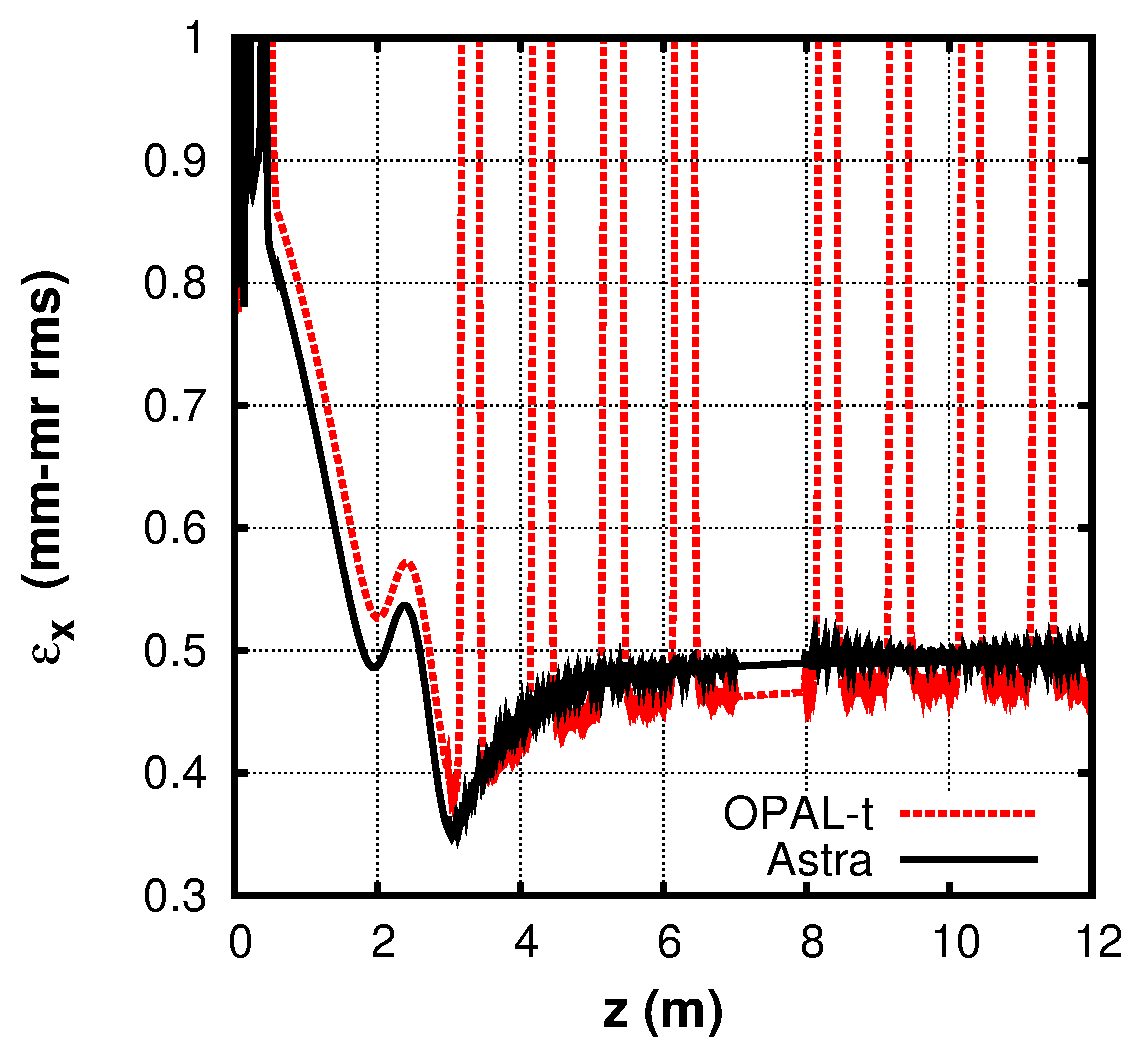
\includegraphics[width=.6\linewidth,angle=0]{figures/opal-astra-sc-exrms-1}
%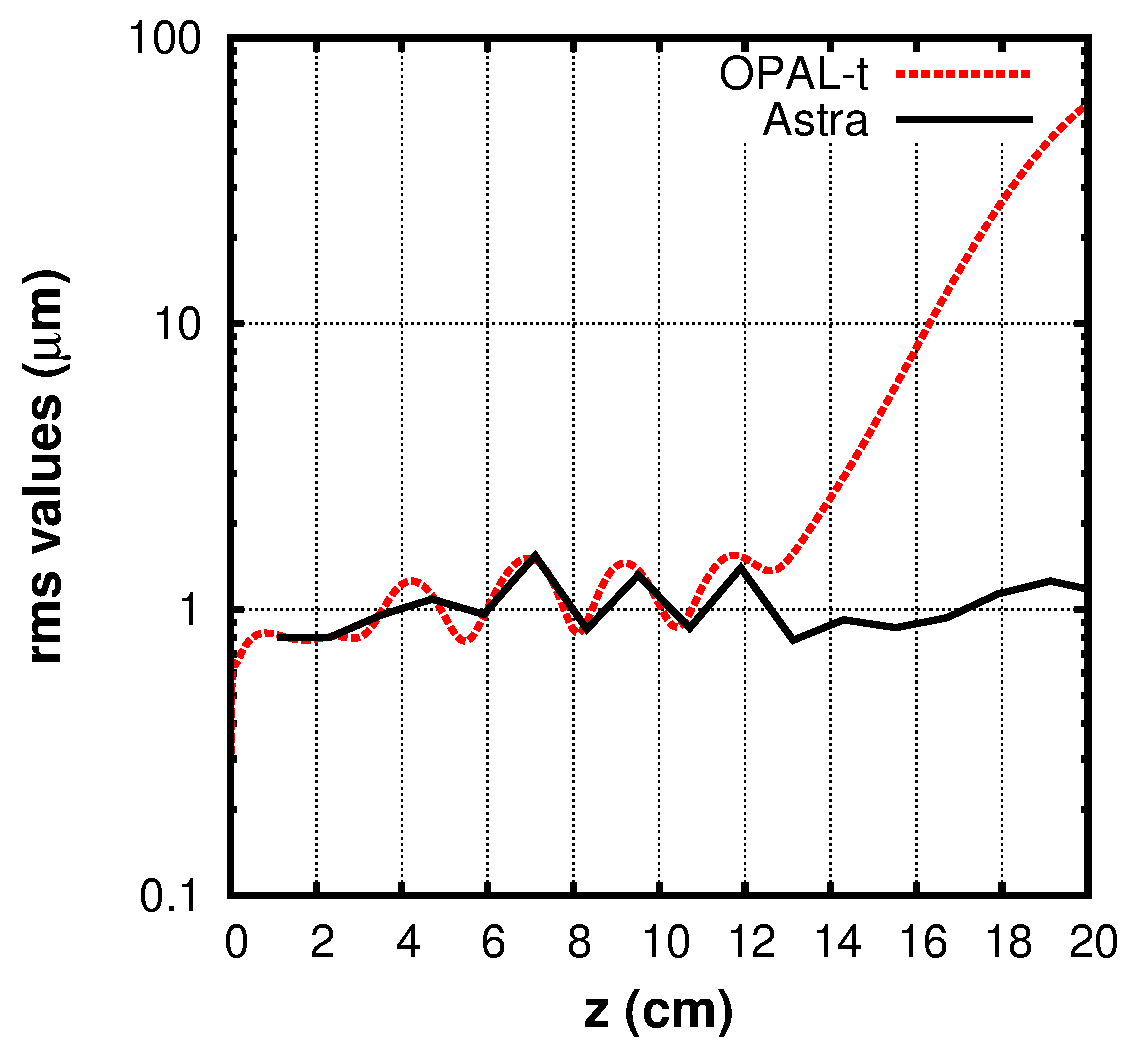
\includegraphics[width=.49\linewidth,angle=0]{figures/opal-astra-sc-exrms-2}
\caption{ RMS beam sizes in $x$ and $z$ for the full simulation (left) and the gun part (right). The normalized
emittance is shown in the lower figure. }
\label{fig:opal-astra-nosc-rmsvals-1}
\end{center}
\end{figure}
\clearpage
\section{\opalt\ \& \opale} \label{sec:tt-vs-et}
We run the envelope-tracker with a slightly modified FWHM to get the same
initial condition as for \opalt\ and get a good match w.r.t. the no
space-charge case (see Fig. \ref{fig:tt_et_nosc}).
\begin{figure}[htbp]
\begin{center}
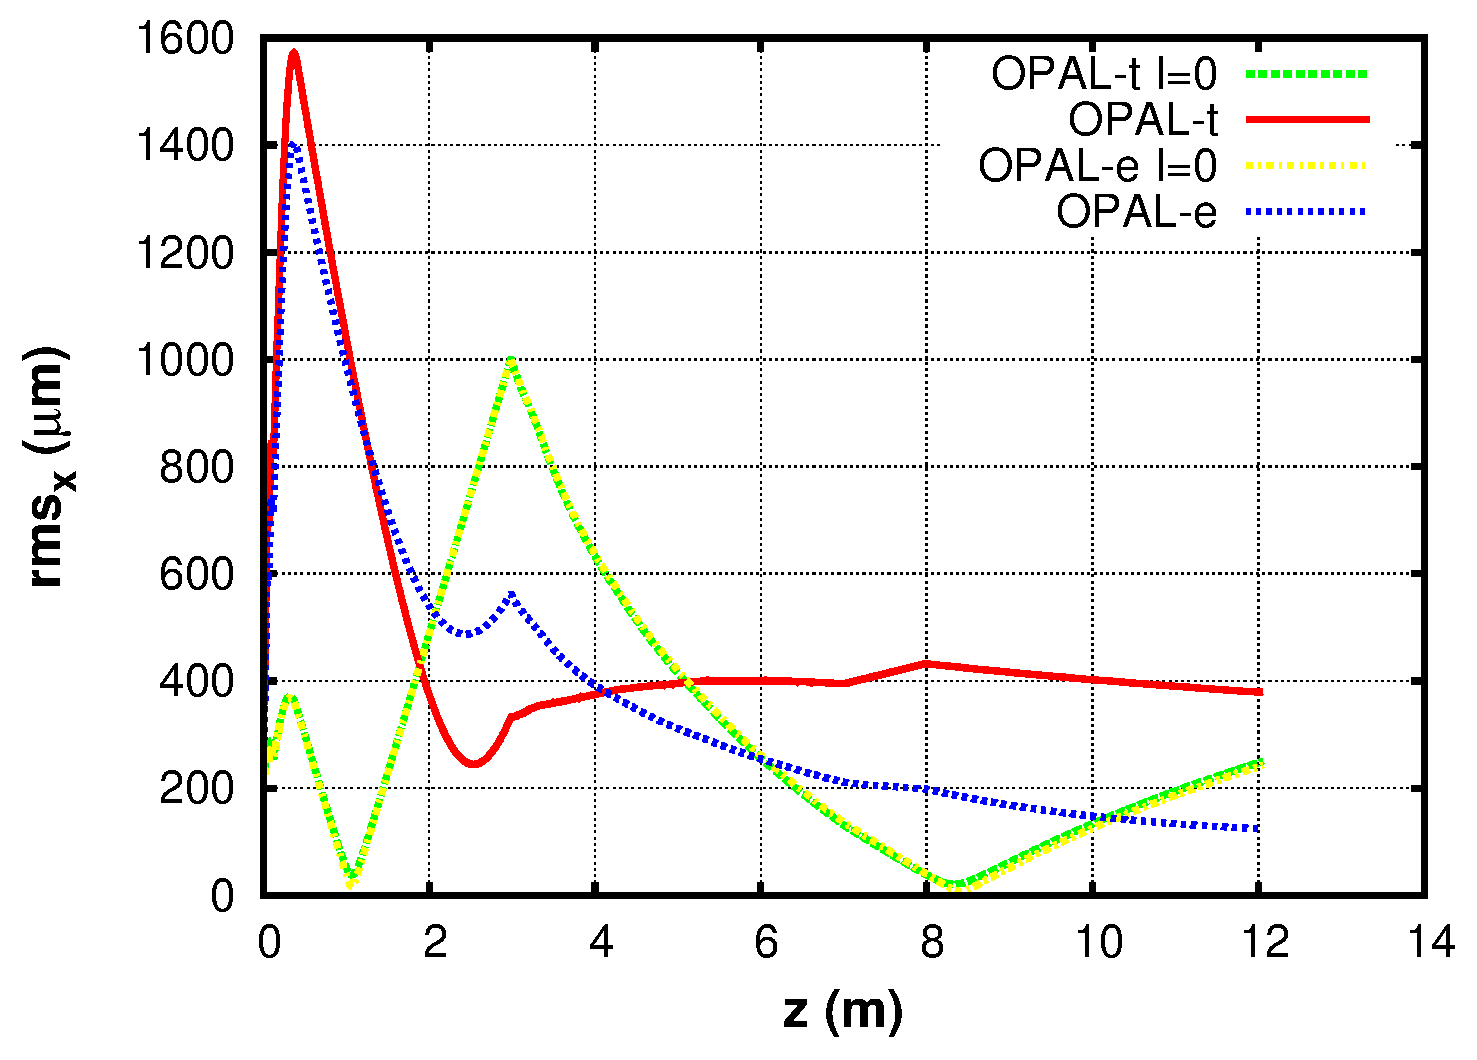
\includegraphics[width=.4\linewidth]{figures/et-tt-xrms}
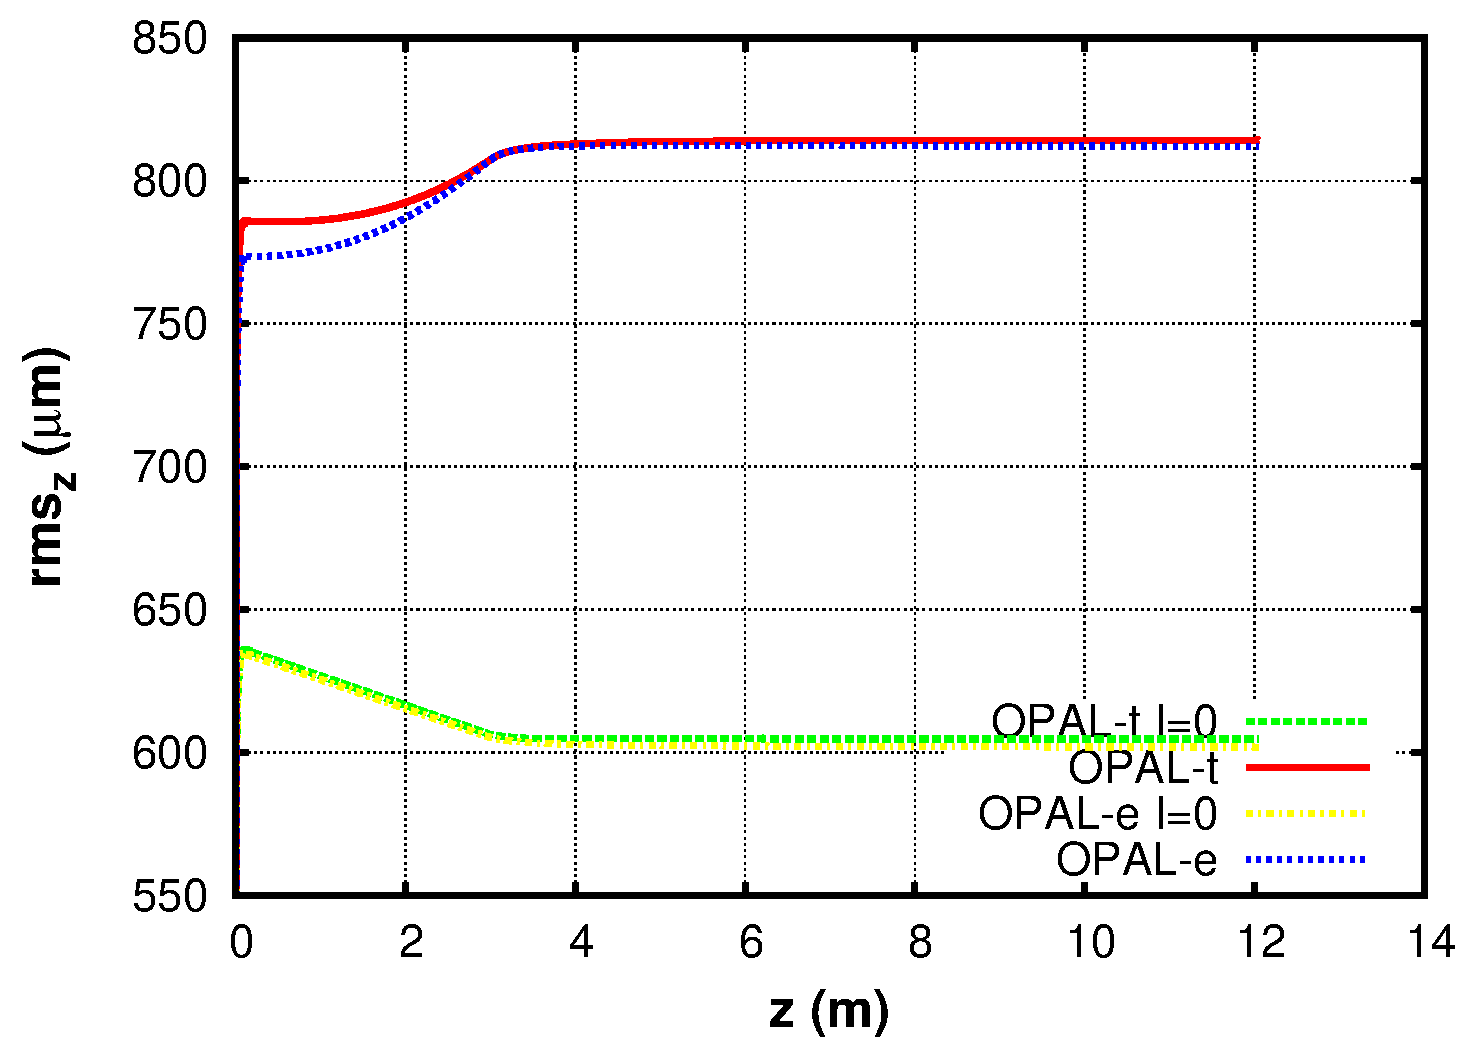
\includegraphics[width=.4\linewidth]{figures/et-tt-zrms}
\caption{\textsc{Left} RMS beam size in $x$ and \textsc{Right} RMS beam size in $z$
of \opalt and \opale. Note that for \opale we use a FWHM of \unit{9.6
\times 10^{-12}}{ps} in the case with space-charge and \unit{8.5\times10^{-12}}{ps} in the case 
without space-charge, whereas in \opalt we have \unit{9.9\times 10^{-12}}{ps}. In the
emittance for \opalt the rotational fields of the solenoids are included.}
\label{fig:tt_et_nosc}
\end{center}
\end{figure}
For the simulation with space-charge we see differences in RMS~$x$. It seems
obvious that something is wrong with the transverse space-charge calculation in \opale. In
the near future we will validate space-charge computation to see if the
differences stem from differences in the space-charge model or are induced by a
bug in the space-charge calculation.

The energy shown in Fig. \ref{fig:tt_et_energy} matches well. Differences are
well below the $1\%$ level.
\begin{figure}[htbp]
\begin{center}
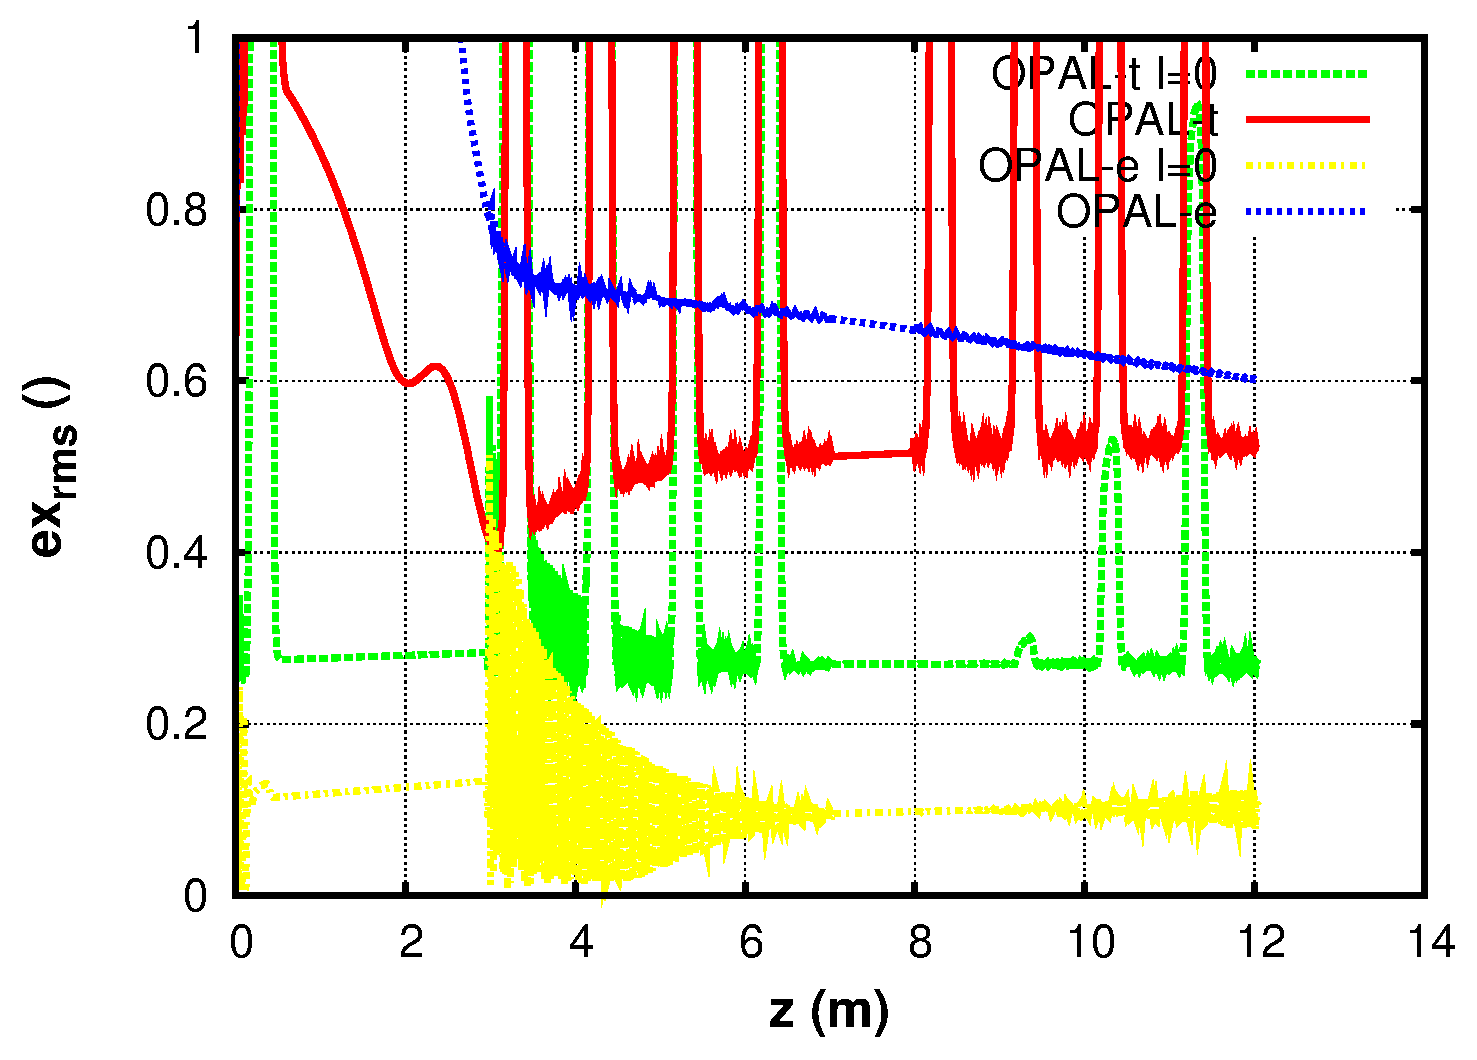
\includegraphics[width=.4\linewidth]{figures/et-tt-exrms}
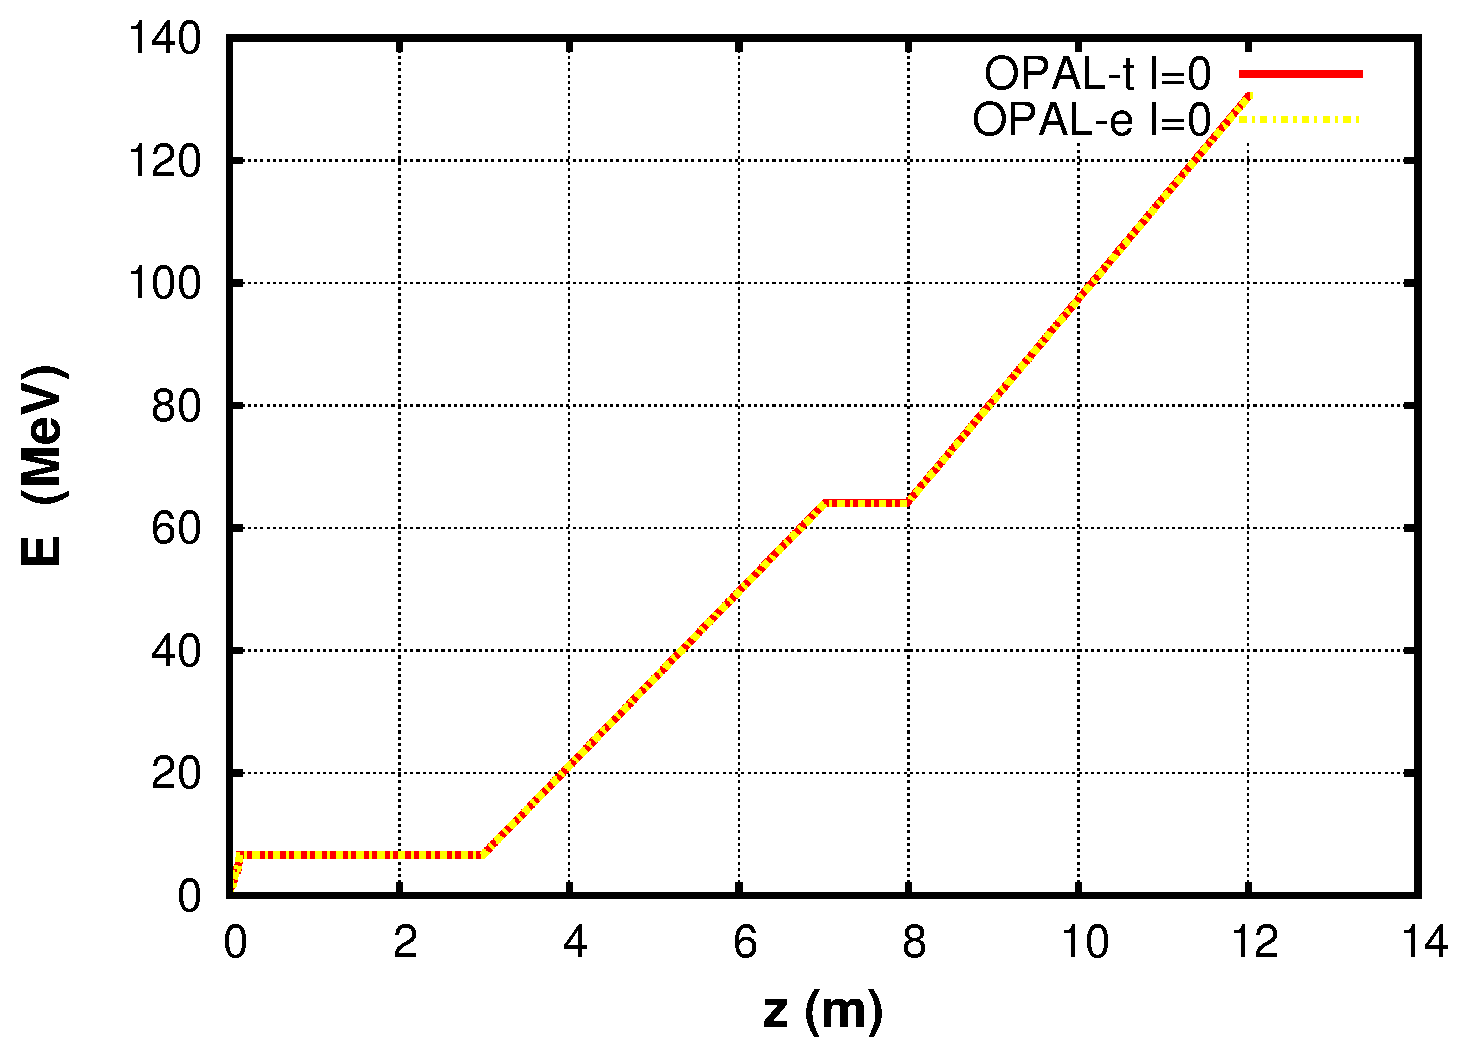
\includegraphics[width=.4\linewidth]{figures/et-tt-energy}
\caption{\textsc{Left}: RMS emittance of \opalt and \opale. \textsc{Right}: Energy of \opalt and \opale.}
\label{fig:tt_et_energy}
\end{center}
\end{figure}

\section{\opal-T \& IMPACT-T} \label{sec:OPALImpactt}

The data presented are based on old versions of both IMPACT-T and \opalt. We
resist from presenting absolute values until we have redone the tests with
the newest version of IMPACT-T. However we can note an overall excellent
agreement, specially with the full 3D field solver. 

\subsection{Drift Test} \label{sec:Drift}

A $1~\mbox{MeV}$ electron beam with $Q=0.0219 ~ \mbox{nC}$ is drifting up to
$0.1~\mbox{m}$ and then entering a solenoid. Momenta and normalised emittance
are compared in Figure~\ref{fig:dr-opal-1}. 
\begin{figure}[htbp]
\begin{center}
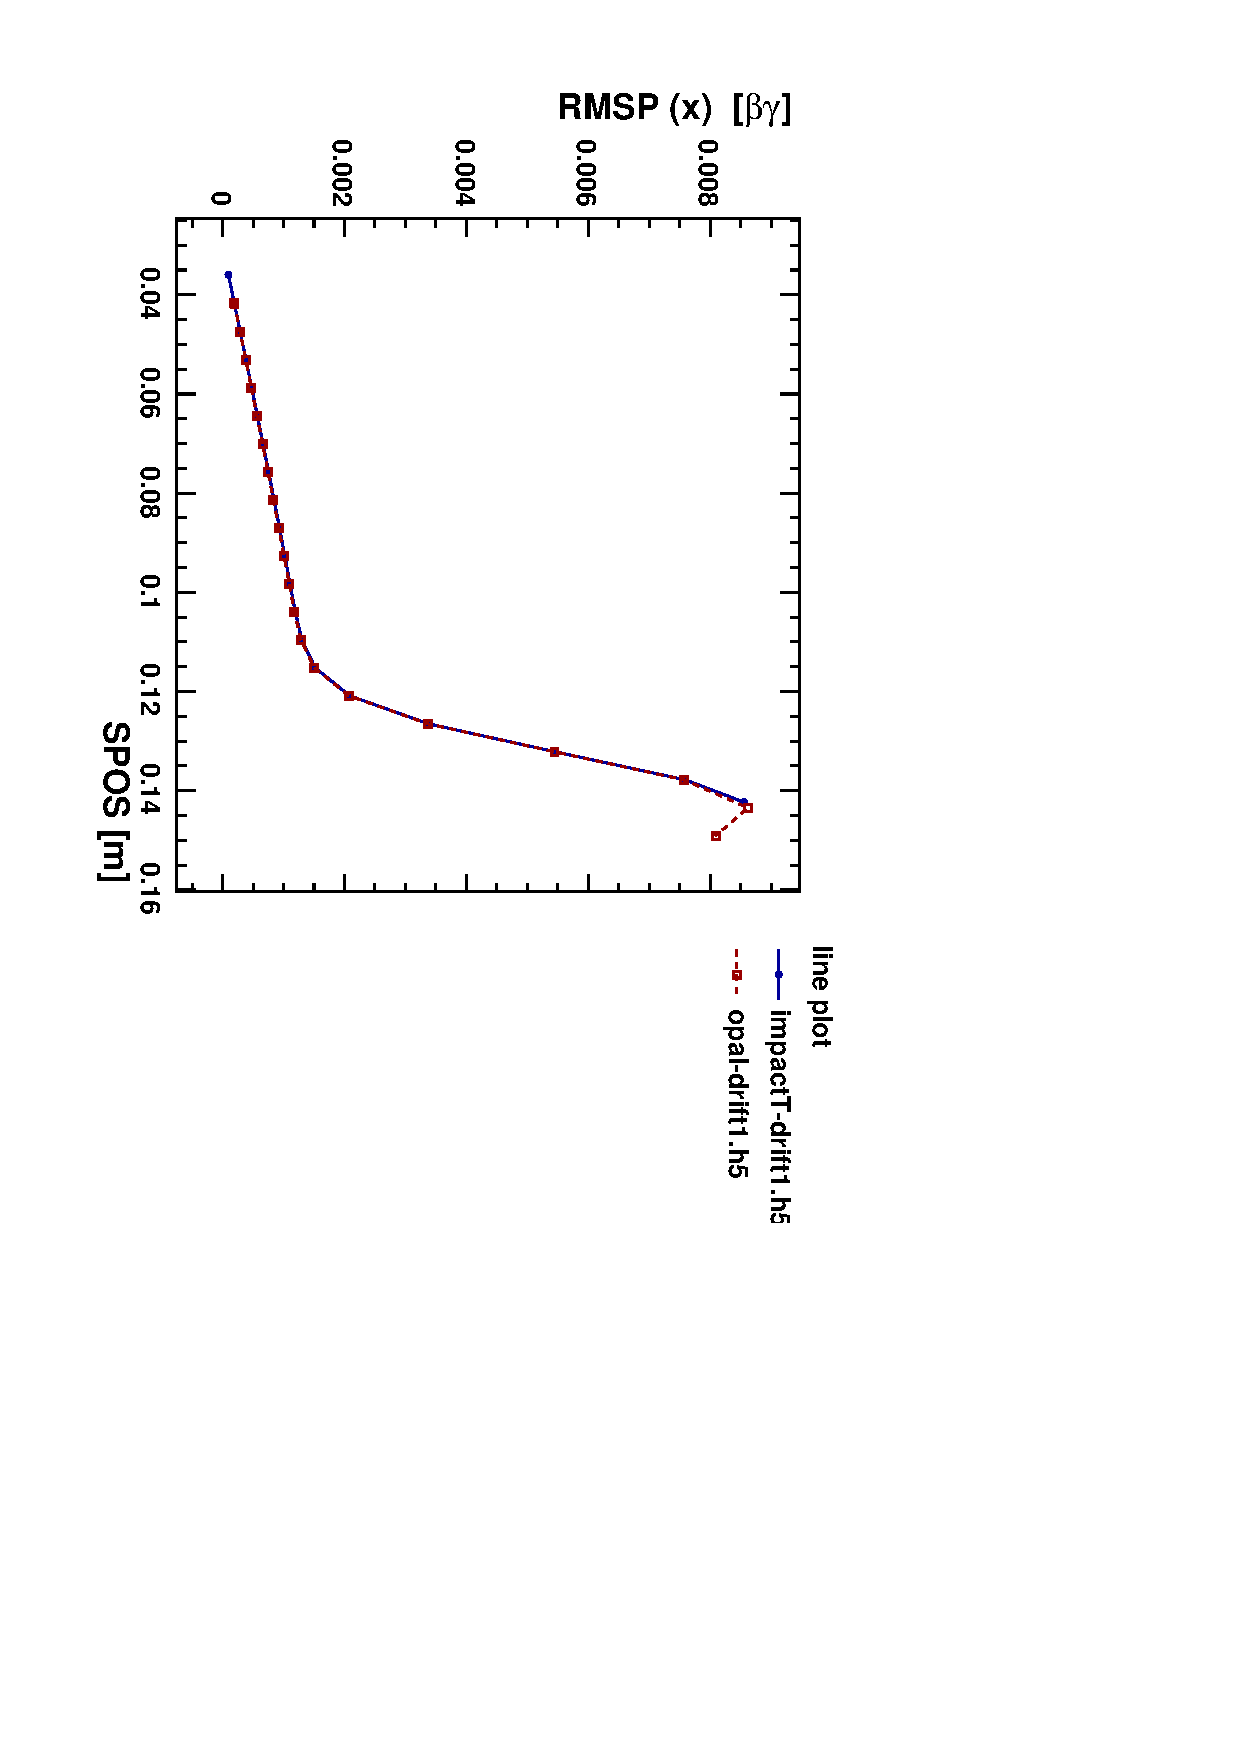
\includegraphics[width=.35\linewidth,angle=90]{figures/impactT-drift1-opal-drift1-RMSP-x-SPOS}
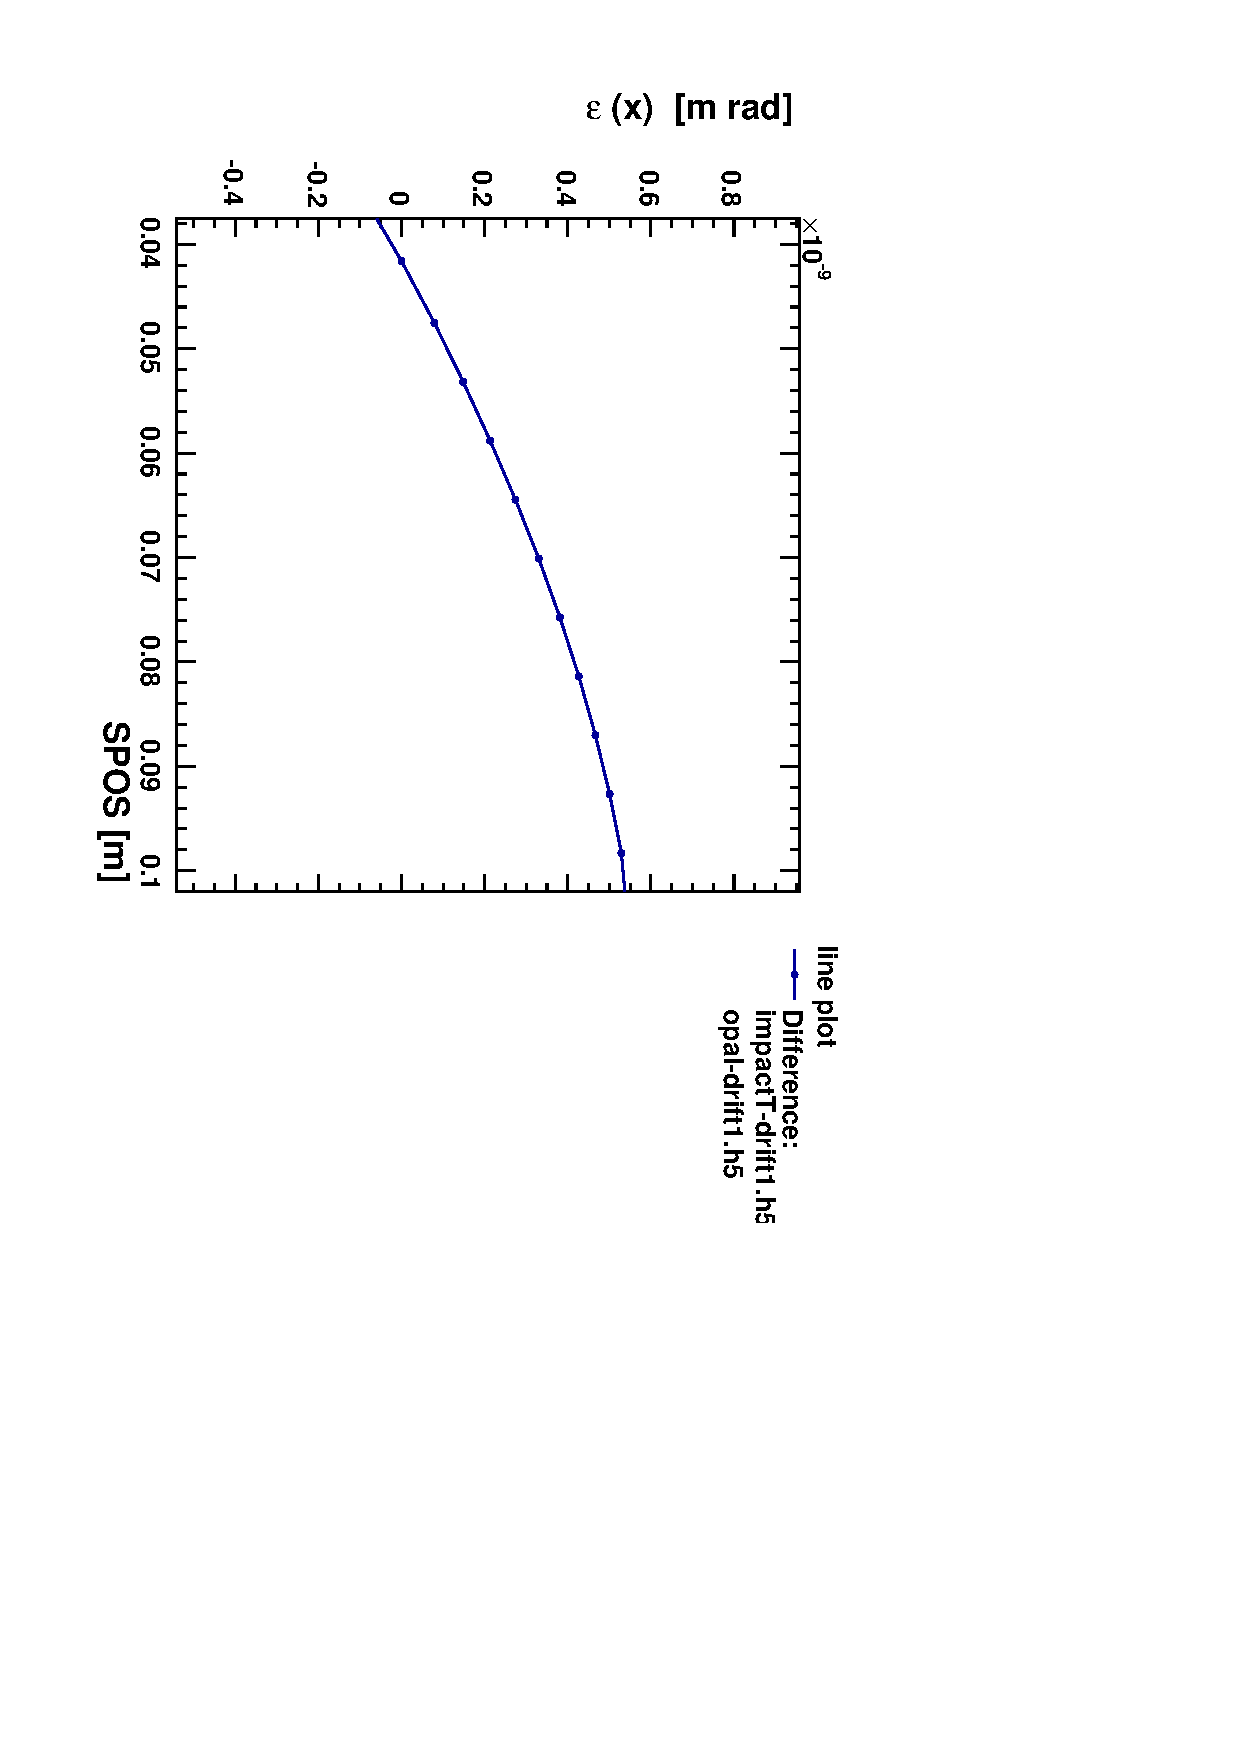
\includegraphics[width=.35\linewidth,angle=90]{figures/impactT-drift1-opal-drift1-varepsilon-x-SPOS}
\caption{RMS momenta in $x$ of \opalt (left red) and IMPACT-T. Difference of normalized RMS emittance in $x$ between \opalt  and IMPACT-T (right)}
\label{fig:dr-opal-1}
\end{center}
\end{figure}

\subsection{Gun Test}      \label{sec:Gun}   
We use the following initial conditions for the OBLA $Q=6 ~ \mbox{pC}$ case with
a $12~\mbox{mm}$ gap. The laser pulse is Gaussian with a $\sigma=6.5~\mbox{ps}$
and a total emission time of $39~\mbox{ps}$. The peak voltage of the pulse is
$500~\mbox{kV}$.
\clearpage
\subsubsection{Gun Test without Space Charge} 
\begin{figure}[htbp]
\begin{center}
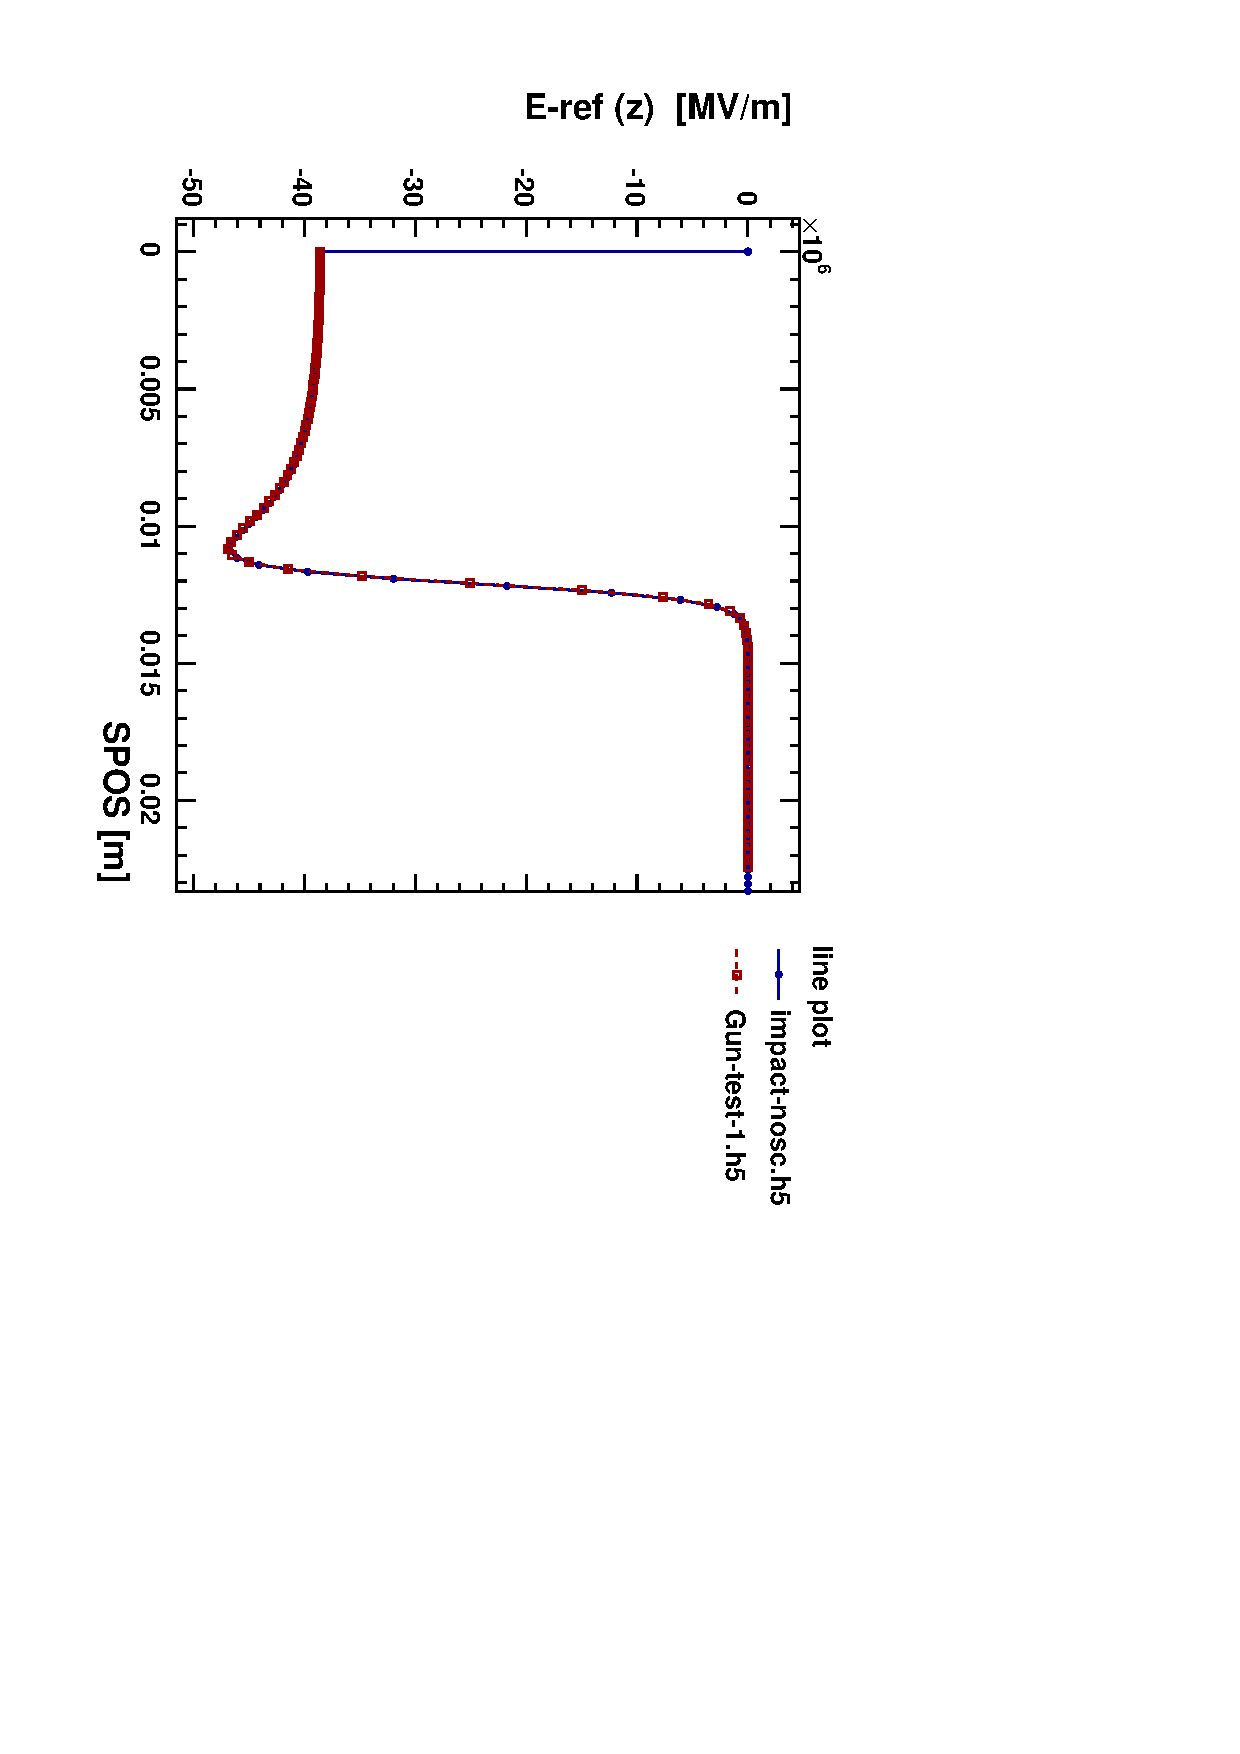
\includegraphics[width=.3\linewidth,angle=90]{figures/impact-nosc-Gun-test-1-E-ref-z-SPOS}
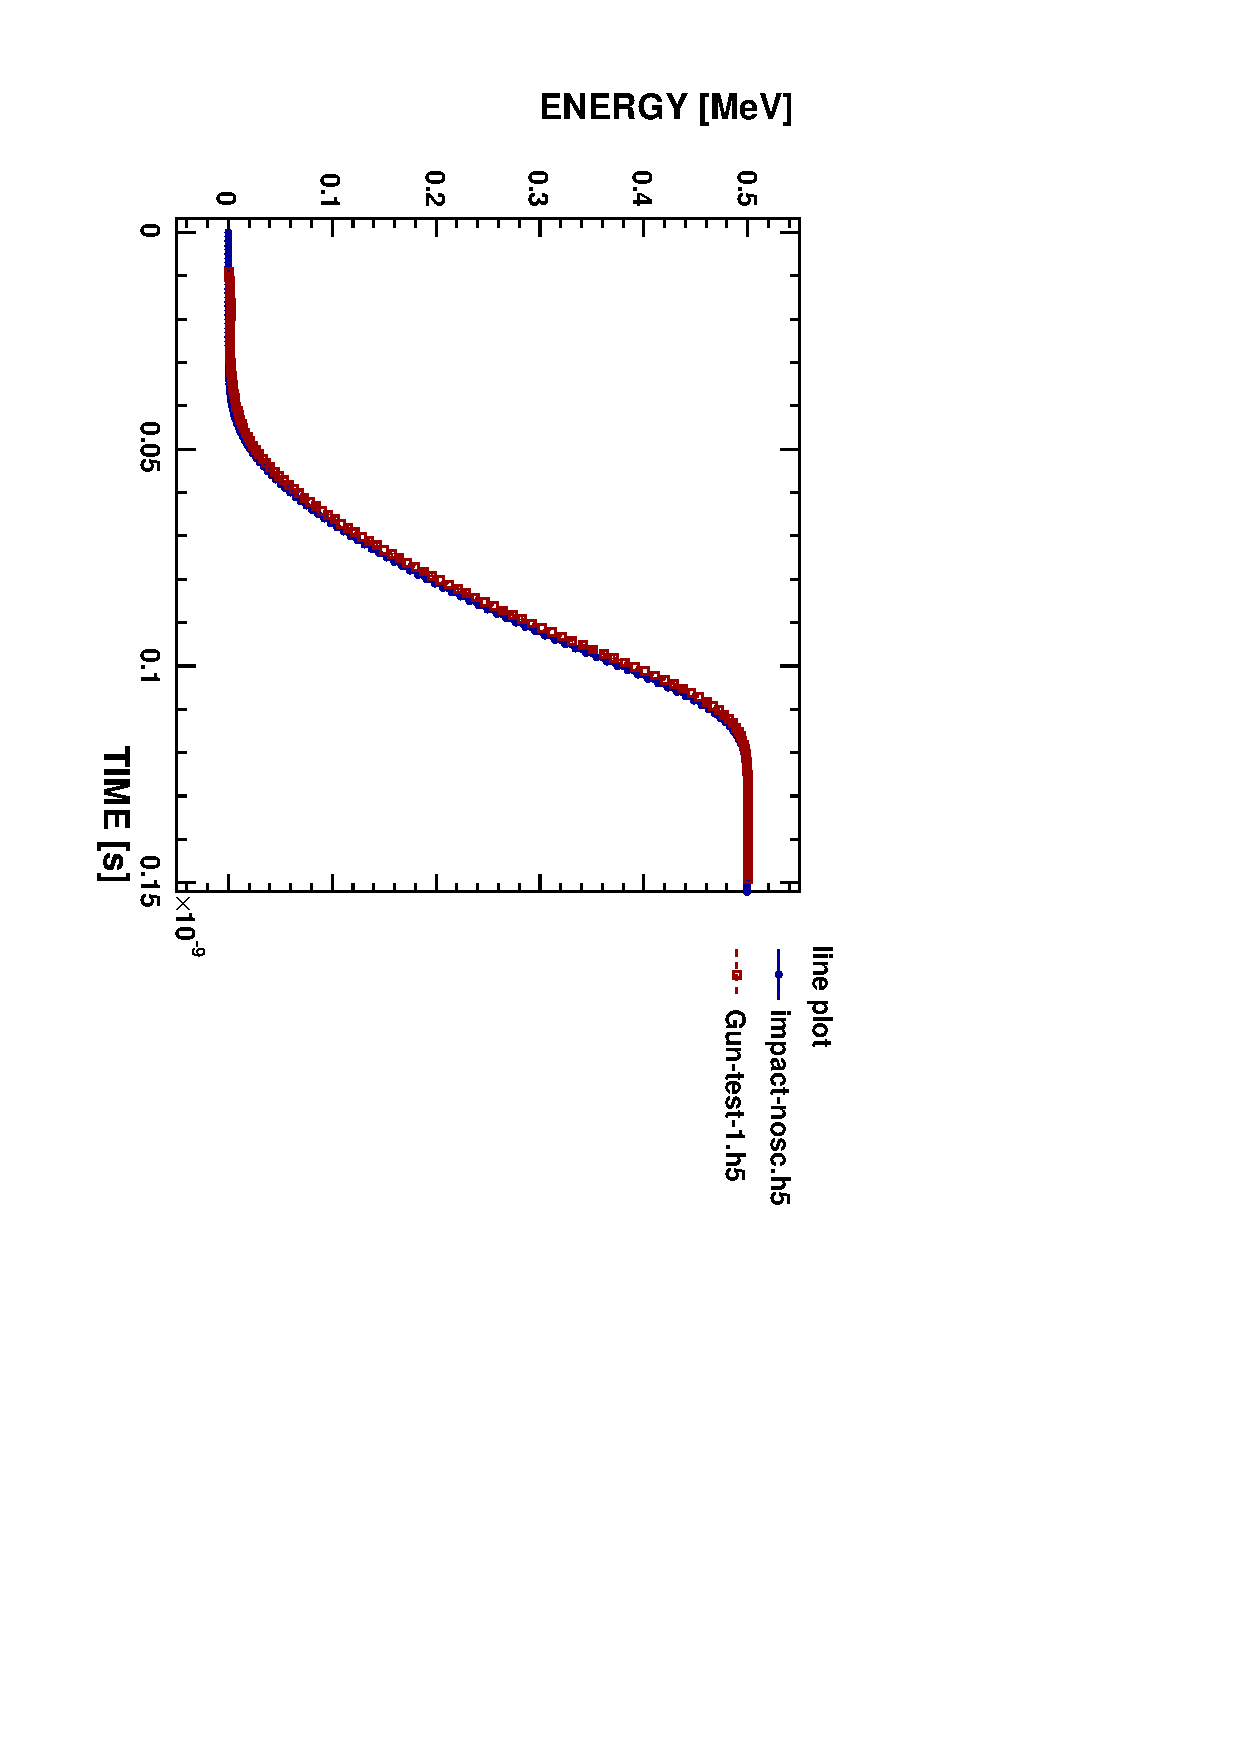
\includegraphics[width=.3\linewidth,angle=90]{figures/impact-nosc-Gun-test-1-ENERGY-TIME}
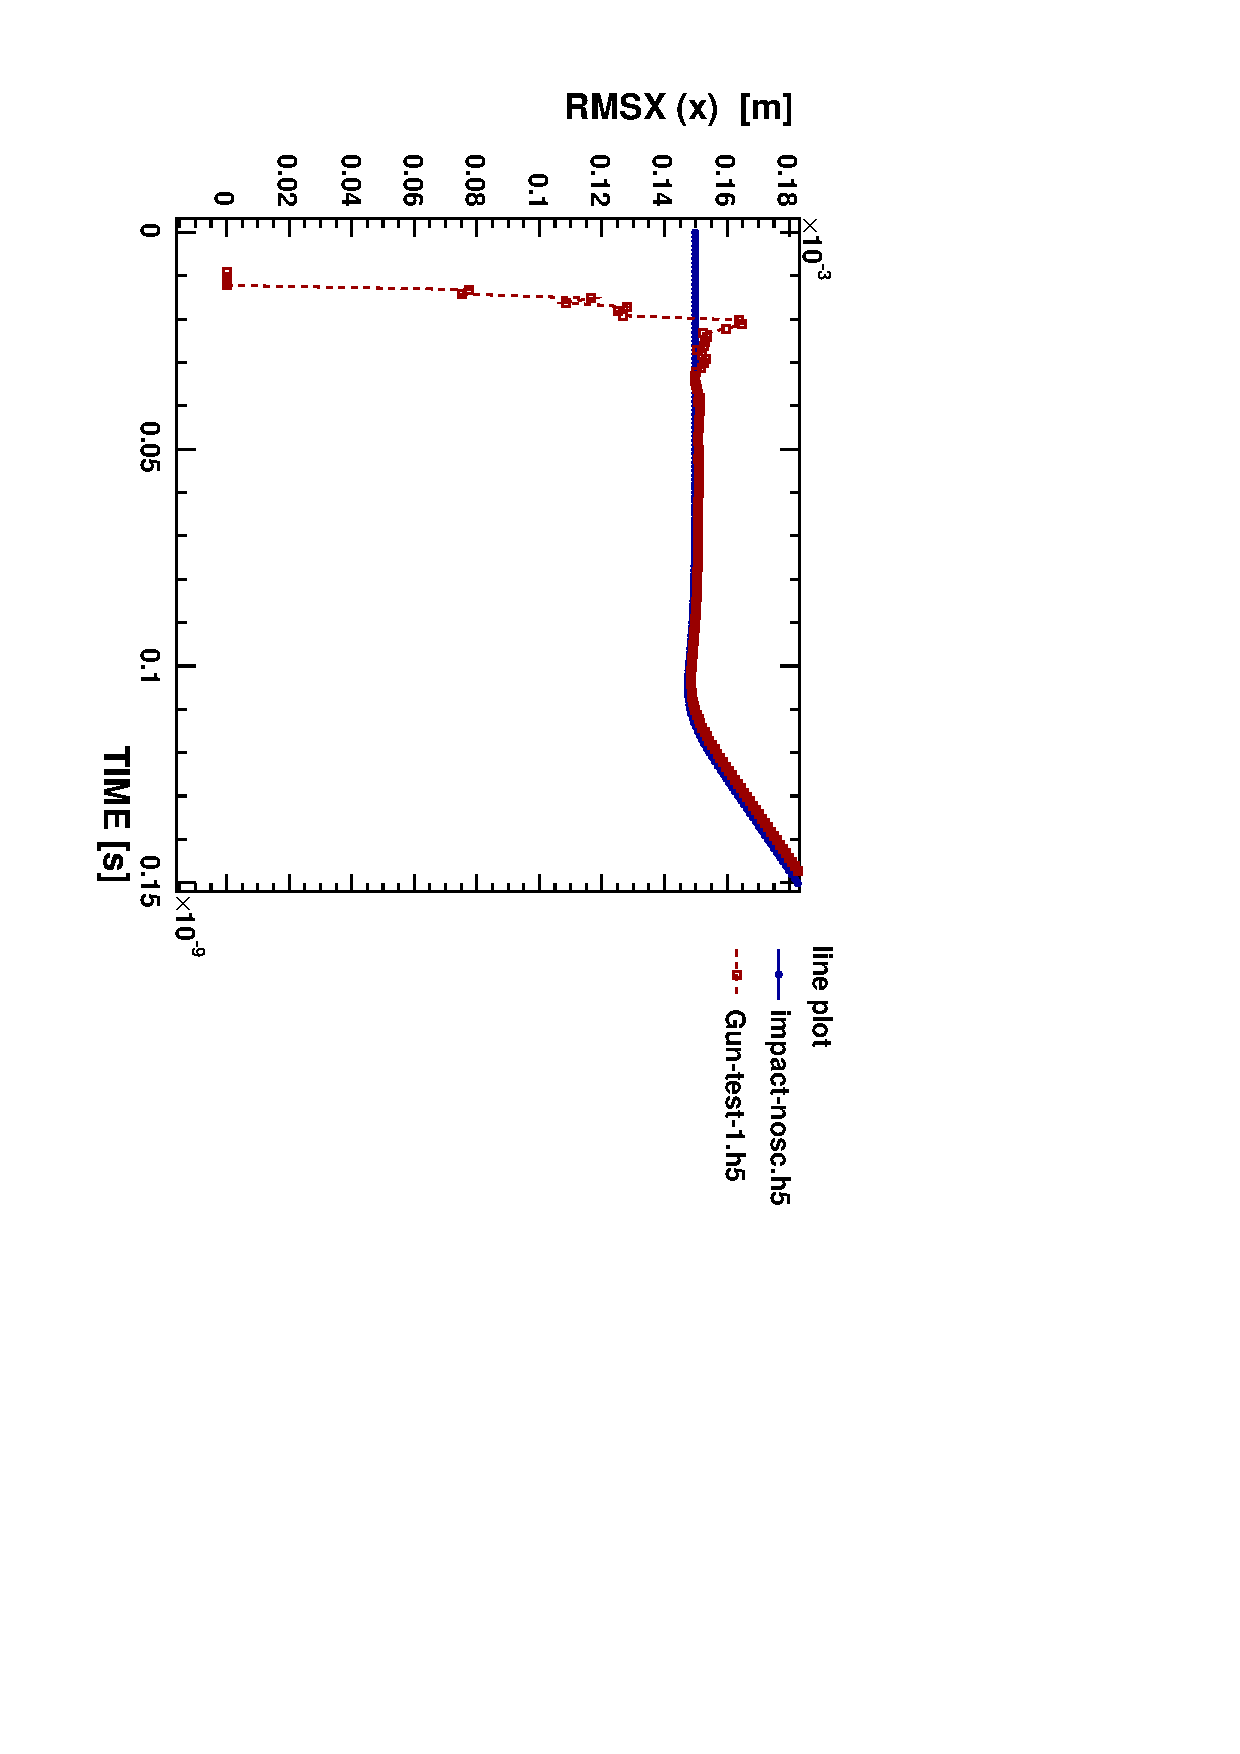
\includegraphics[width=.3\linewidth,angle=90]{figures/impact-nosc-Gun-test-1-RMSX-x-TIME}
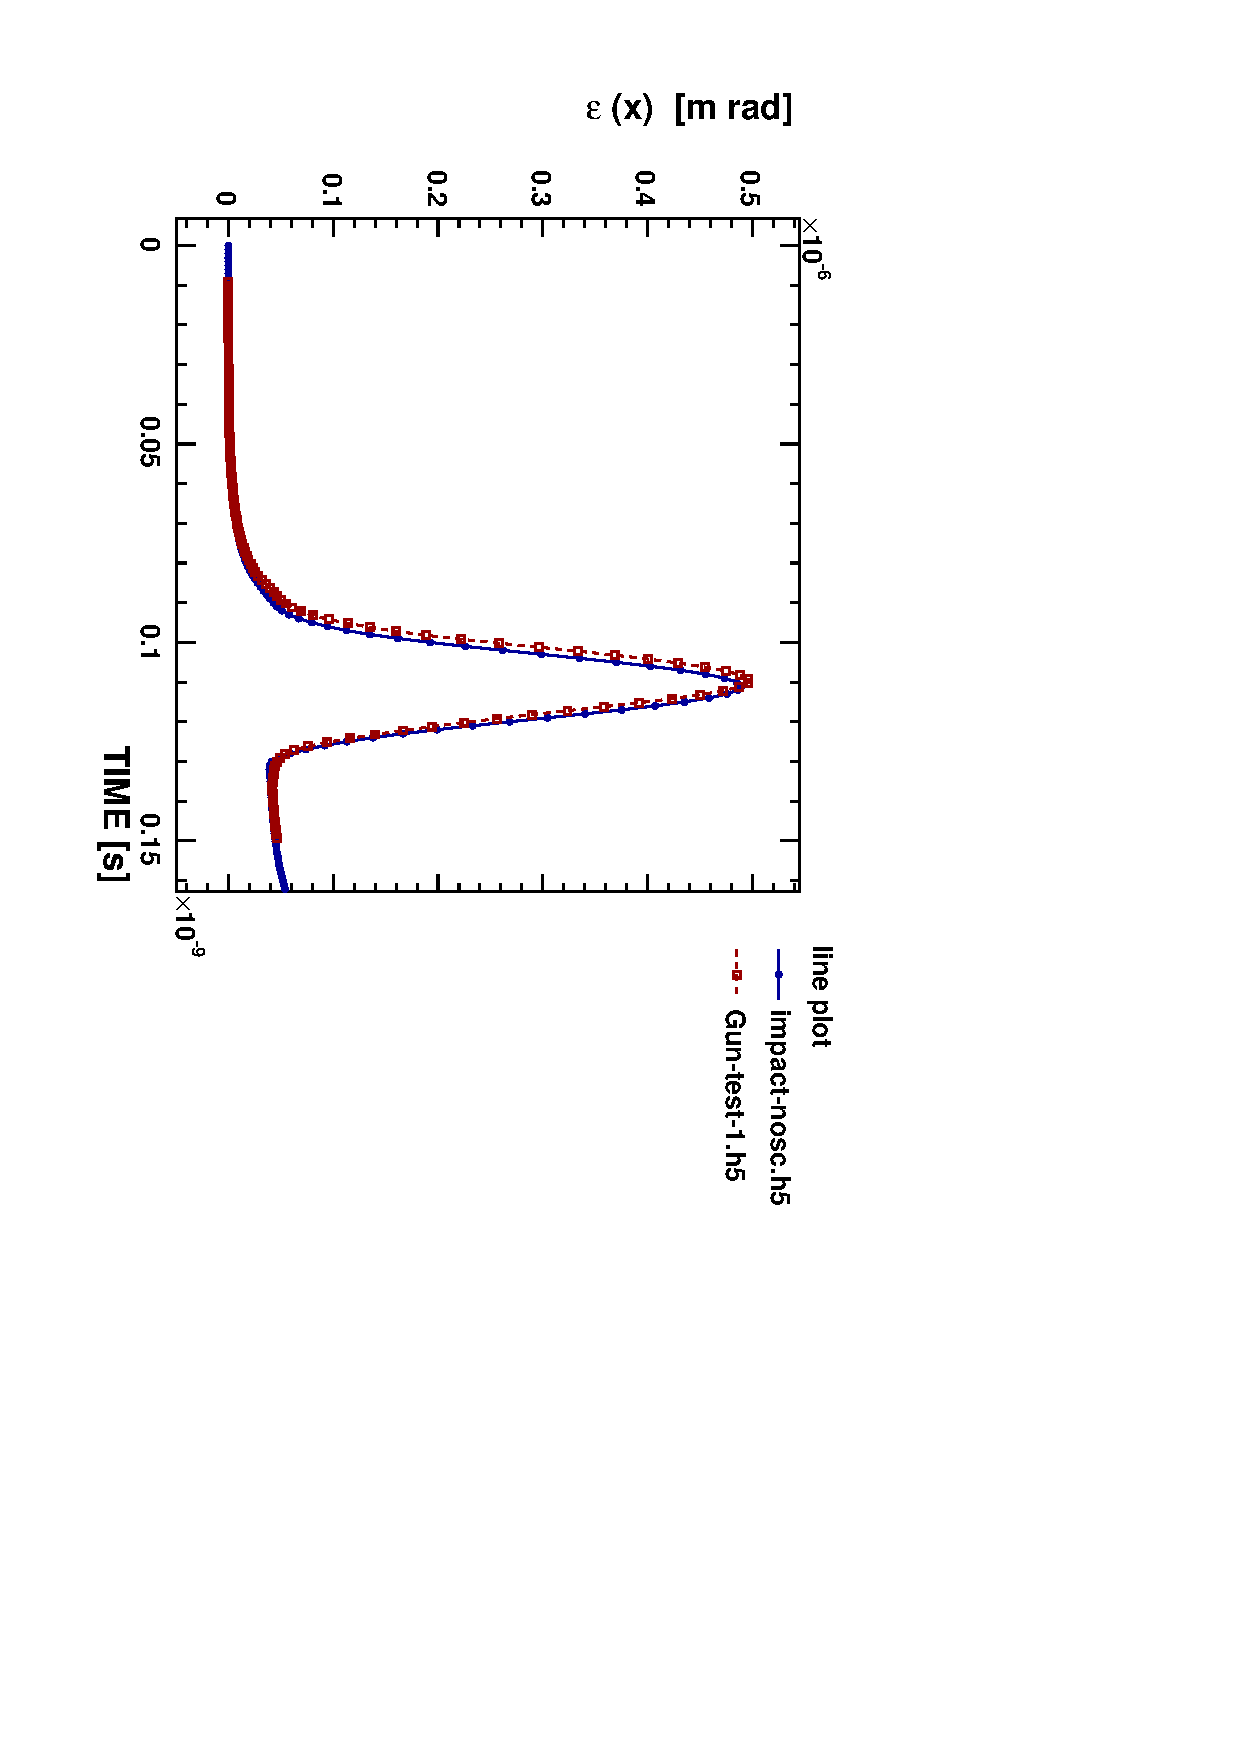
\includegraphics[width=.3\linewidth,angle=90]{figures/impact-nosc-Gun-test-1-varepsilon-x-TIME}
\vspace{-5mm}
\caption{Longitudinal electrical field seen by the particle in the middle of the bunch (upper left) and  mean energy gain over the \unit{12}{mm} gap. RMS~$x$ (lower left) and normalised emittance $\epsilon_{xn}$.}
\label{fig:gun-opal-1}
\end{center}
\end{figure}

\pagebreak
\subsubsection{Gun Test with Space Charge}
\begin{figure}[htbp]
\begin{center}
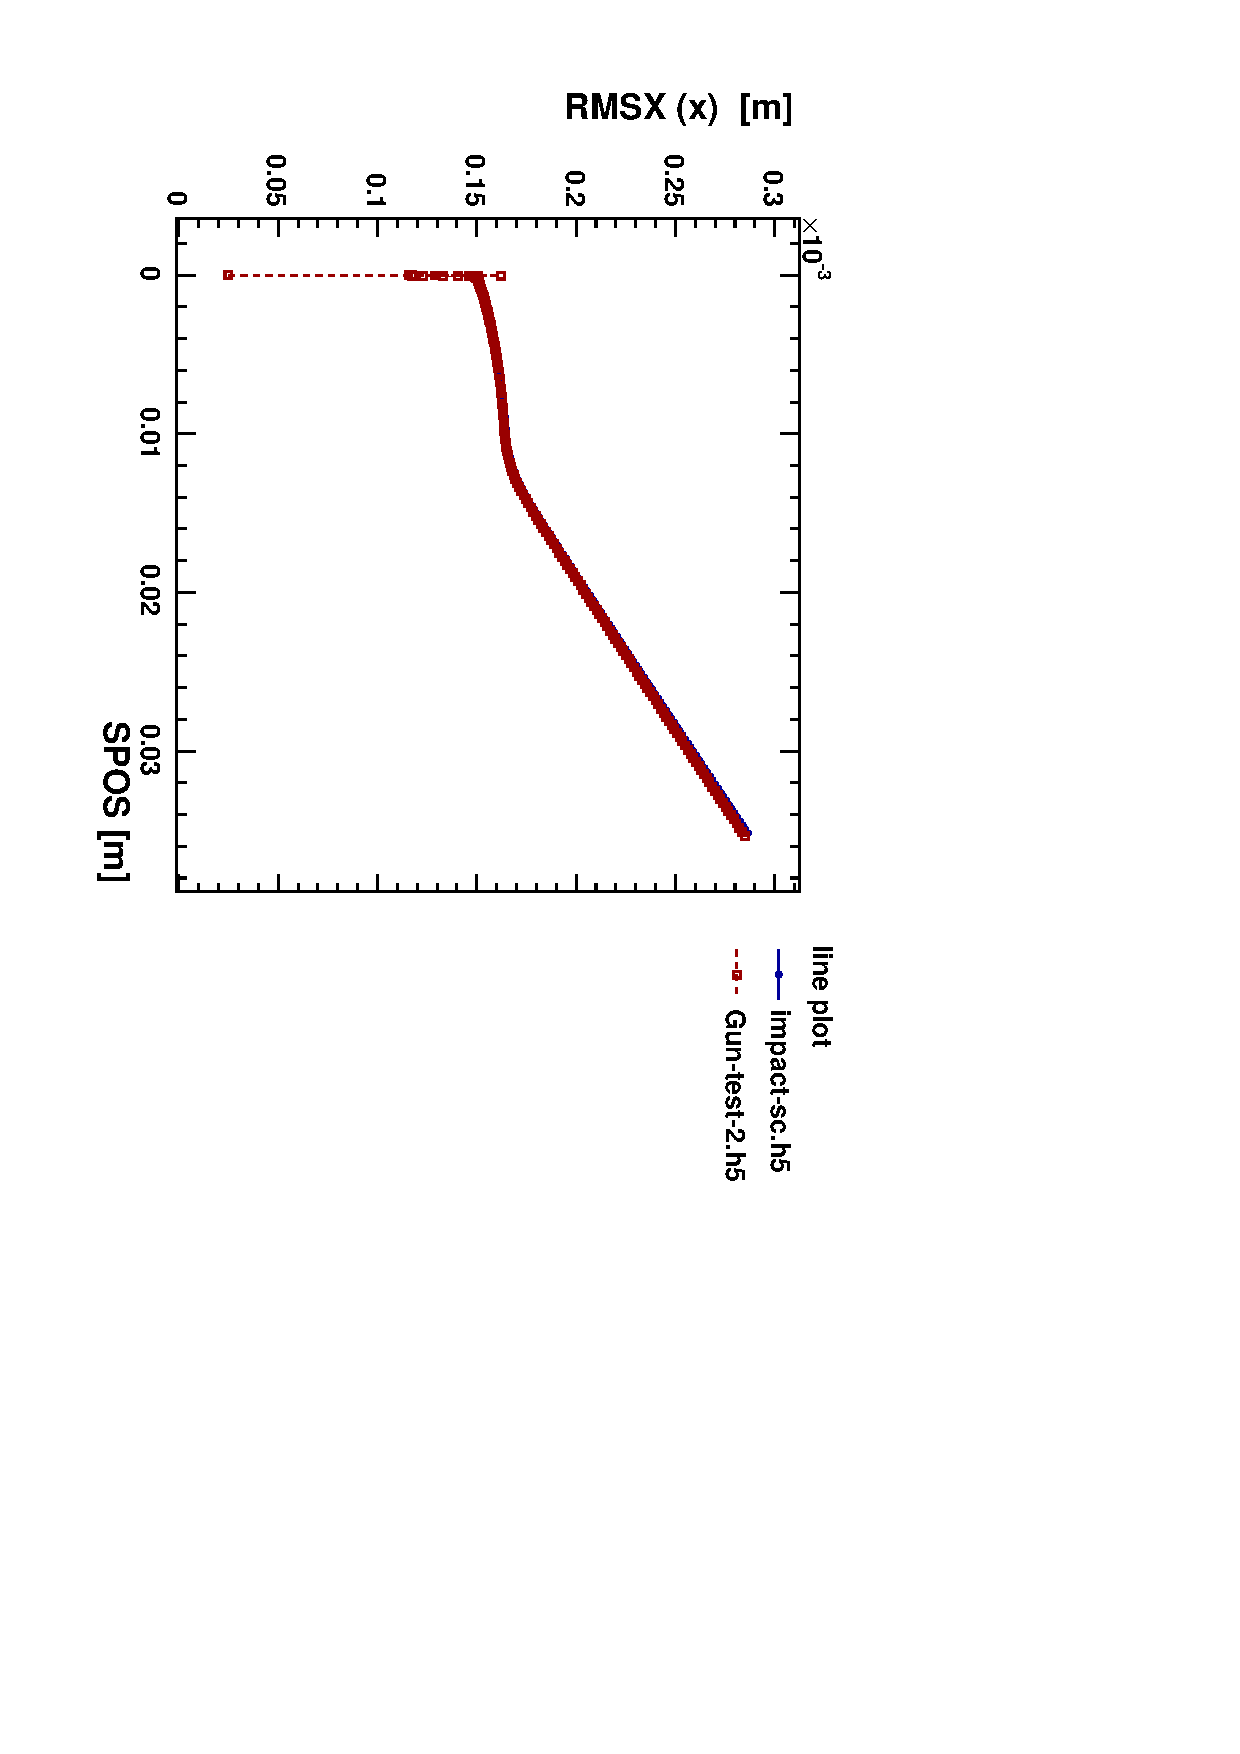
\includegraphics[width=.3\linewidth,angle=90]{figures/impact-sc-Gun-test-2-RMSX-x-SPOS}
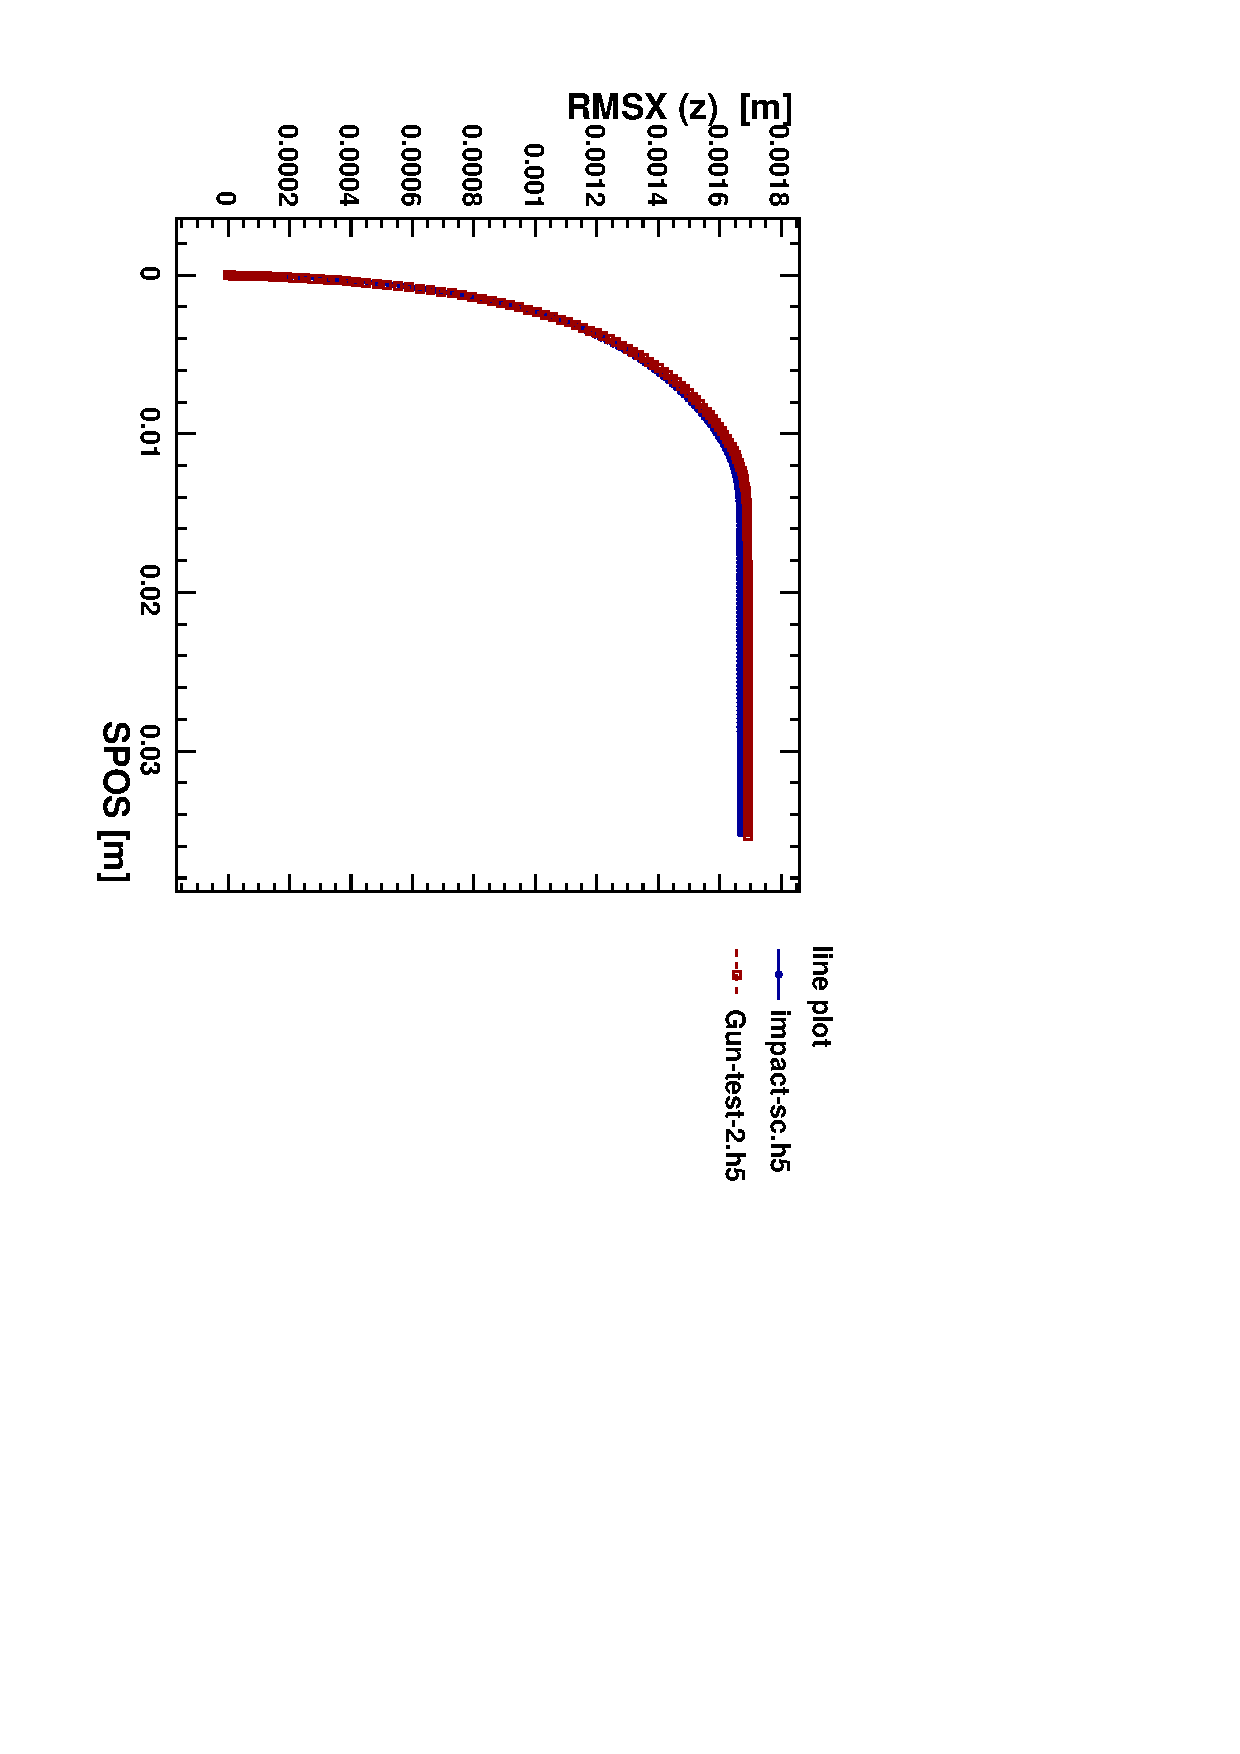
\includegraphics[width=.3\linewidth,angle=90]{figures/impact-sc-Gun-test-2-RMSX-z-SPOS}
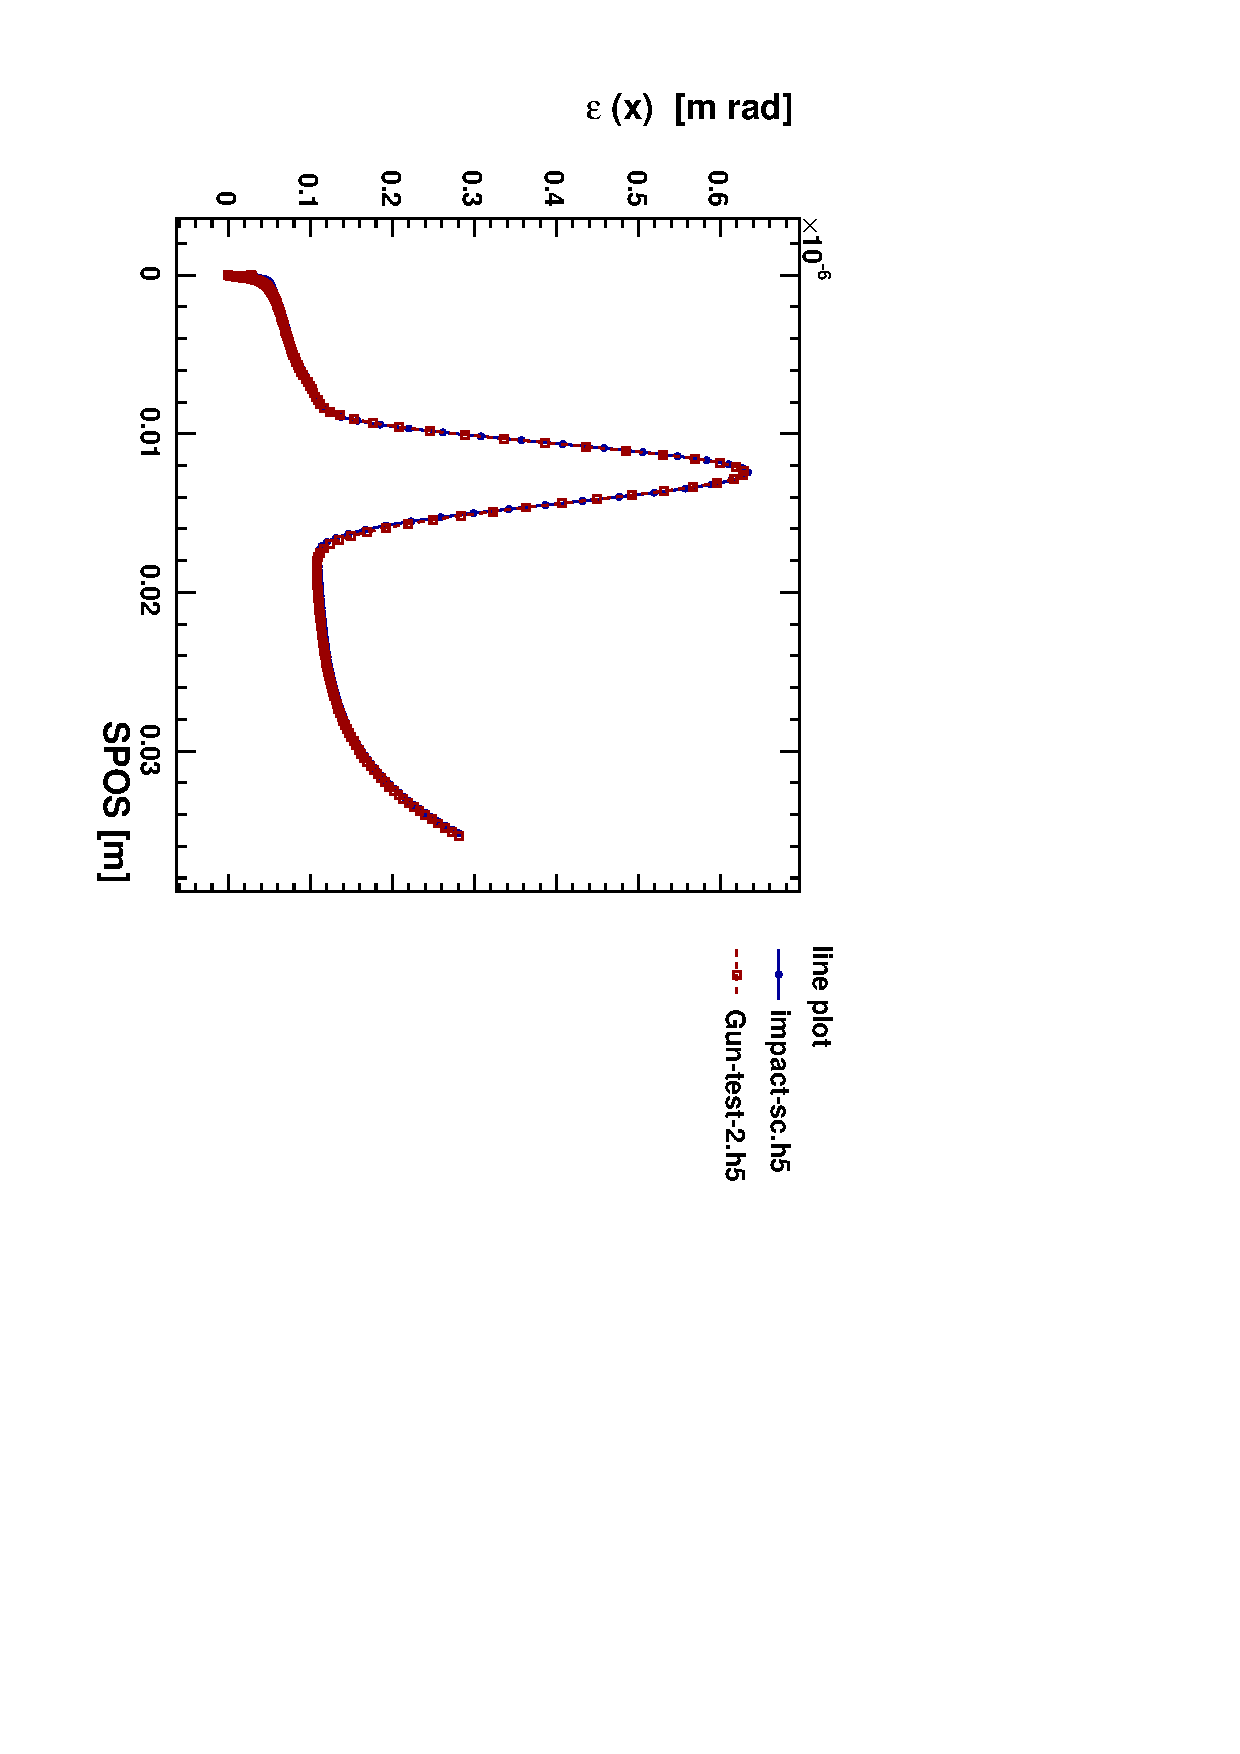
\includegraphics[width=.3\linewidth,angle=90]{figures/impact-sc-Gun-test-2-varepsilon-x-SPOS}
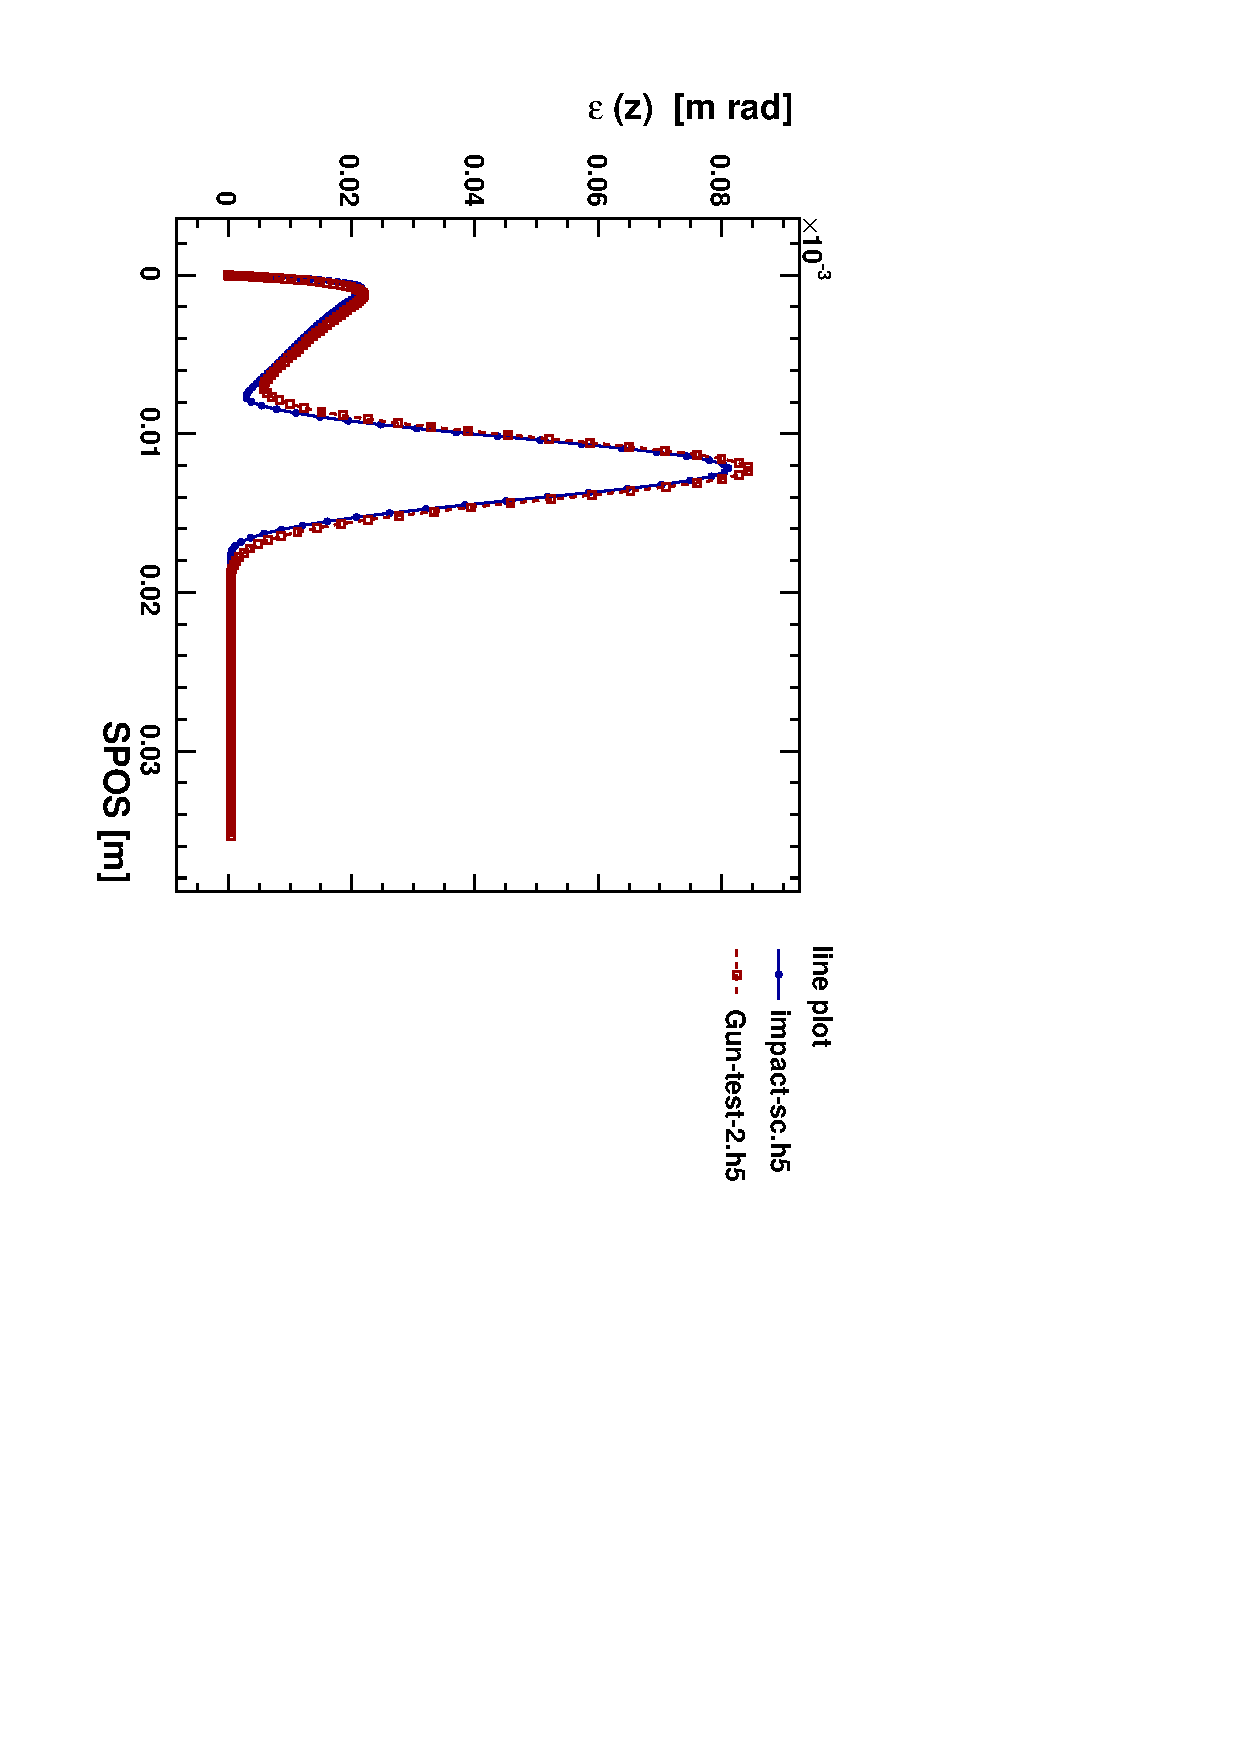
\includegraphics[width=.3\linewidth,angle=90]{figures/impact-sc-Gun-test-2-varepsilon-z-SPOS}
\caption{RMS~$x$ (upper left) and  $z$ beam size, RMS~$\epsilon_{xn}$ (lower left) and  $\epsilon_{zn}$ normalised  emittance. }
\label{fig:gun-opal-5}
\end{center}
\end{figure}
\begin{figure}[htbp]
\begin{center}
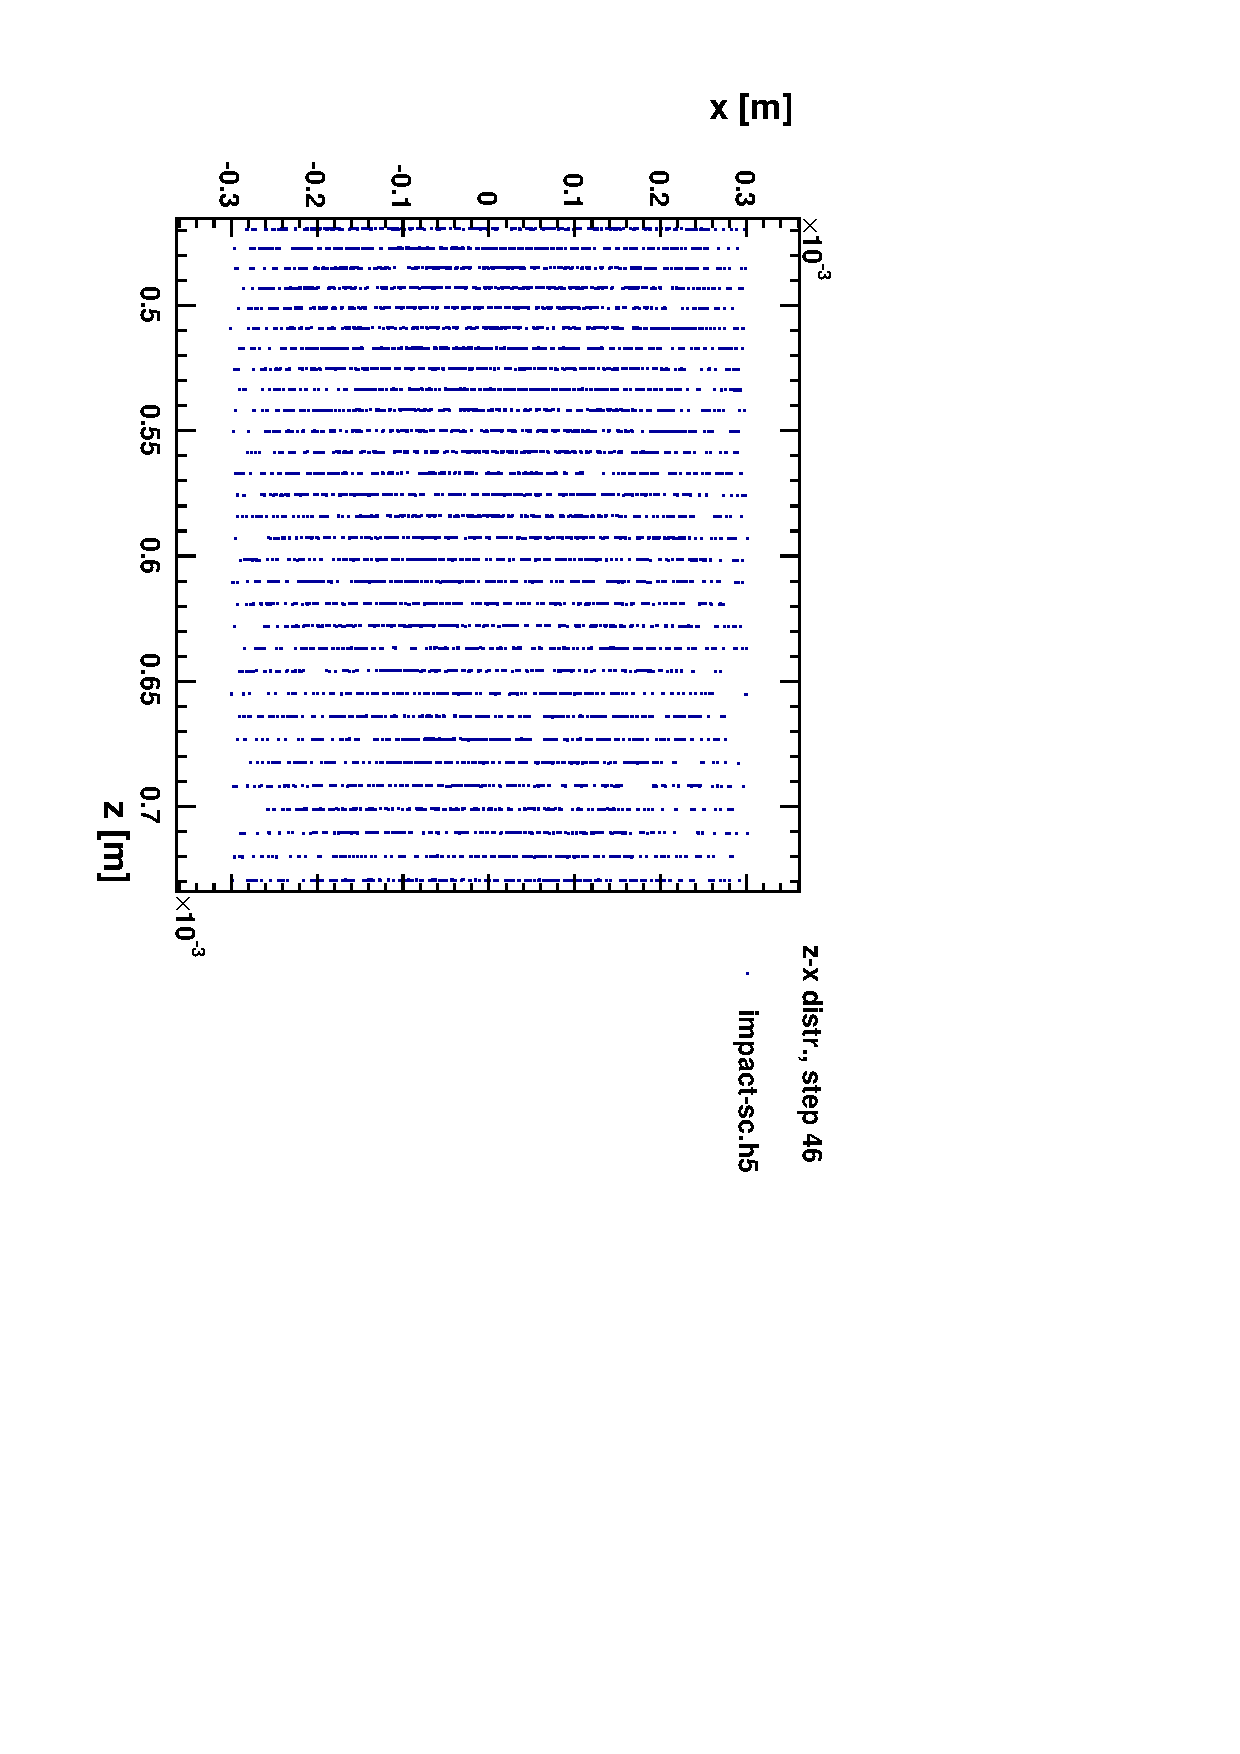
\includegraphics[width=.25\linewidth,angle=90]{figures/impact-test-2-x-z-step-46.pdf}
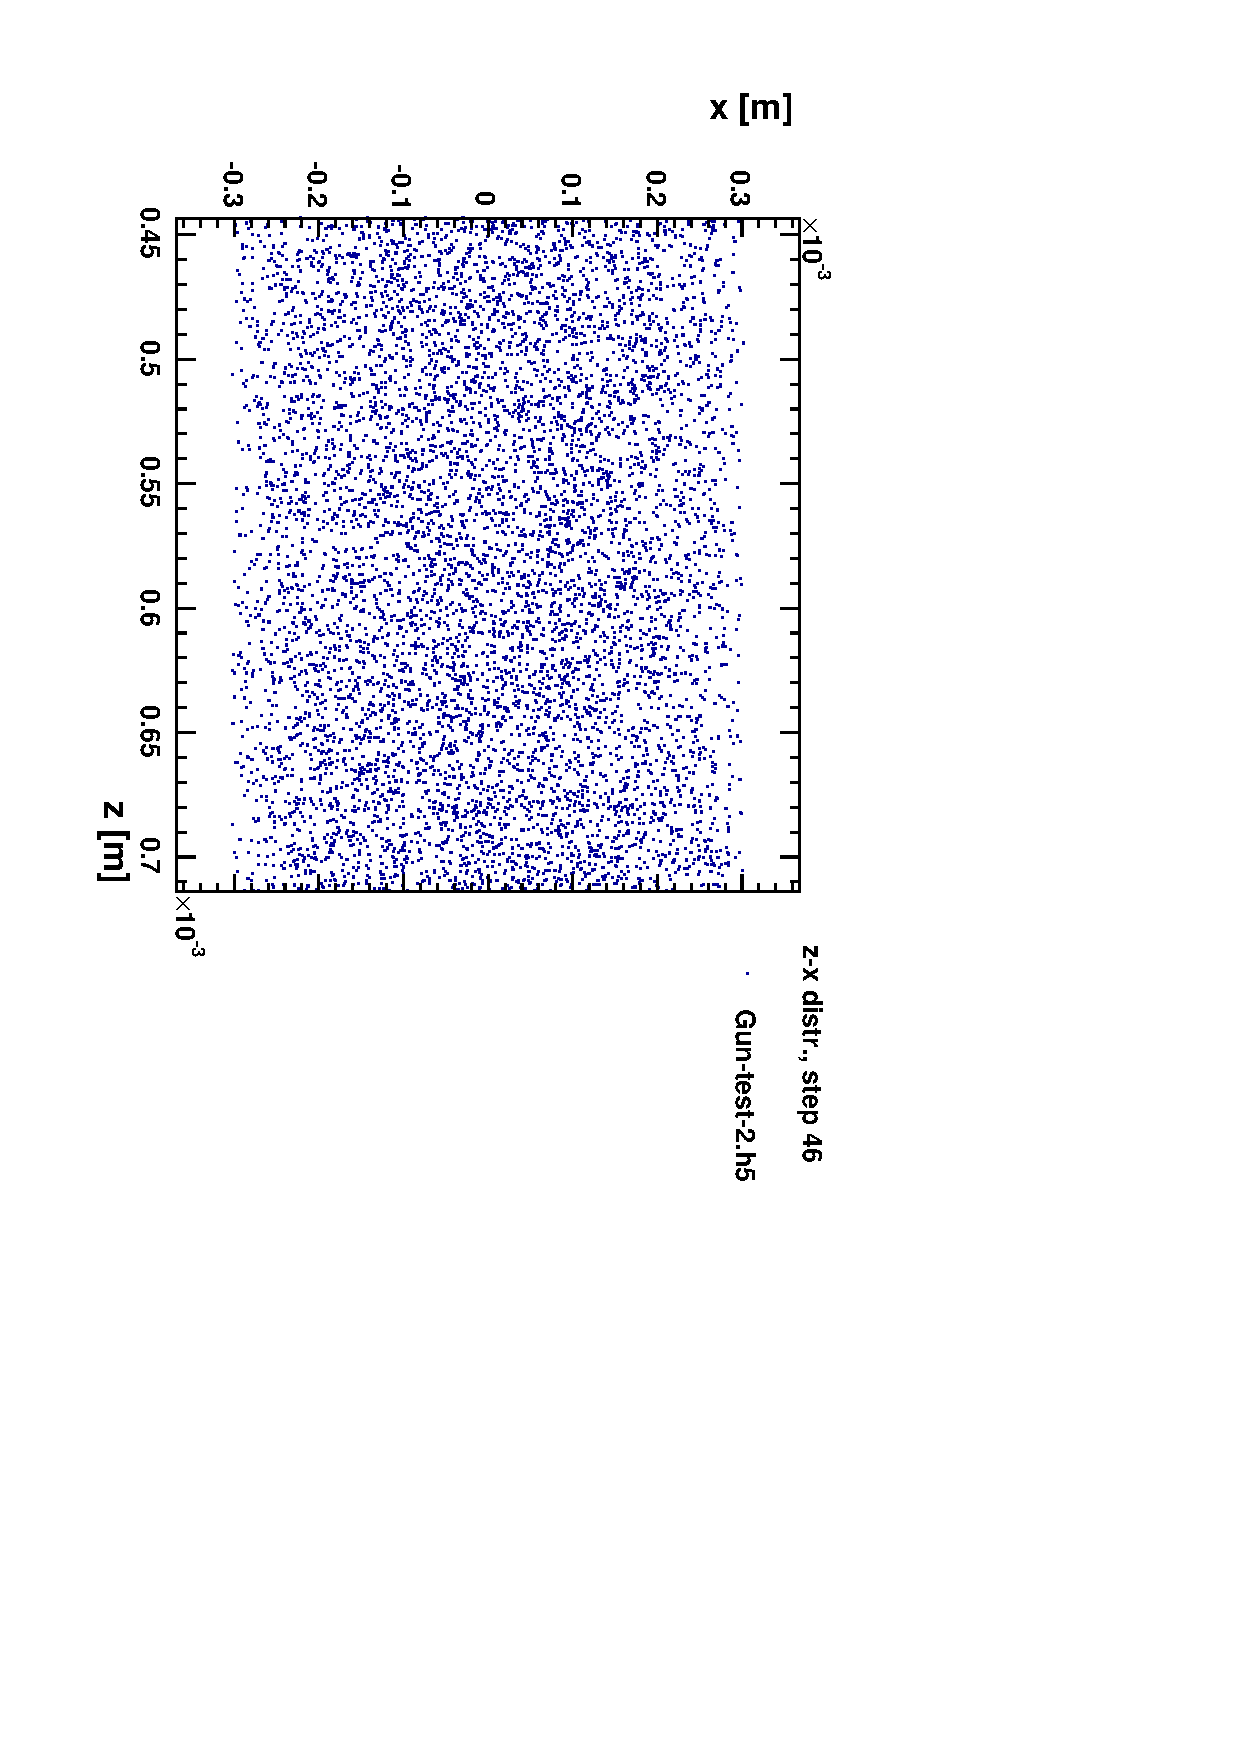
\includegraphics[width=.25\linewidth,angle=90]{figures/Gun-test-2-x-z-step-46.pdf}
\caption{ $(x,z)$ real space plots of IMPACT-T (left) and \opal-t}
\label{fig:gun-opal-6}
\end{center}
\end{figure}


\section{Parallel Efficiency}

The parallel efficiency is defined as $t_n/t_1$ i.e. the ratio of the time on
$n$ processors vs. the time on one processor multiplied by $1/n$.
\begin{equation}
p = \frac{t_n}{t_1}\frac{1}{n} \times 100 \%
\end{equation}


\subsection{\opal\ \& Astra}

We cannot estimate the parallel efficiency of Astra because we use the single
core version. We obtain a {\bf decrease} of the time to solution by a factor of
$\sim \bf 6$ on the problem described in section \ref{sec:OPALAstra} (from 6
hours  down to 1 hour) when running \opal~on the PSI cluster
(felsim) using 16 cores. If you are not require a converged emittance value (in the case you do parameter scans) 
the time to solution can even be further decreased to $30$ to $40$ minutes. 

%\subsection{External Field Test}
%We use the test case from section \ref{sec:ExtFieldSC} but with $200$ time steps only.
%\begin{table}[ht]
%\caption{Parallel Efficiency in \% of \opal-t} on Merlin3 % title of Table
%\centering % used for centering table
%\begin{tabular}{c c c c c c} % centered columns (4 columns)
%\hline\hline %inserts double horizontal lines
%Processors & Wall  & Field Solver & Particle Pusher & I/O & Load Balancing \\ [0.75ex] % inserts table
%%heading
%\hline % inserts single horizontal line
%1 & 100 & 100 & 100 & 100 & 100\\ % inserting body of the table
%2 & 47 & 877 & 230 & (,) & (,)\\
%4 & 31 & 25 & 415 & (,) & (,)\\
%8 & 35 & 144 & 2356 & (,) & (,)\\
%16 & 45 & 300 & 556 & (,) & (,)\\ [1ex] % [1ex] adds vertical space
%\hline %inserts single line
%\end{tabular}
%\label{table:nonlin} % is used to refer this table in the text
%\end{table}

%\begin{table}[ht]
%\caption{Parallel Efficiency in \% of \opal-t} on Palu (CRAY XT-3/4) % title of Table
%\centering % used for centering table
%\begin{tabular}{c c c c c c} % centered columns (4 columns)
%\hline\hline %inserts double horizontal lines
%Processors & Wall  & Field Solver & Particle Pusher & I/O & Load Balancing \\ [0.75ex] % inserts table
%%heading
%\hline % inserts single horizontal line
%1 & 100 & 100 & 100 & 100 & 100\\ % inserting body of the table
%2 & 47 & 877 & 230 & (,) & (,)\\
%4 & 31 & 25 & 415 & (,) & (,)\\
%8 & 35 & 144 & 2356 & (,) & (,)\\
%16 & 45 & 300 & 556 & (,) & (,)\\ [1ex] % [1ex] adds vertical space
%32 & 45 & 300 & 556 & (,) & (,)\\ [1ex] % [1ex] adds vertical space
%\hline %inserts single line
%\end{tabular}
%\label{table:nonlin} % is used to refer this table in the text
%\end{table}

%\begin{figure}[htbp]
%\begin{center}
%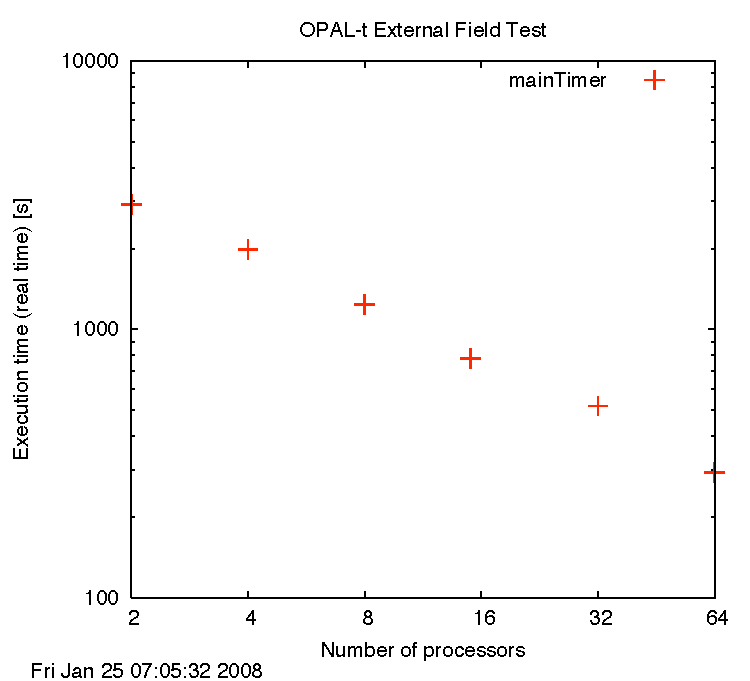
\includegraphics[width=.3\linewidth,angle=0]{figures/mainTimer}
%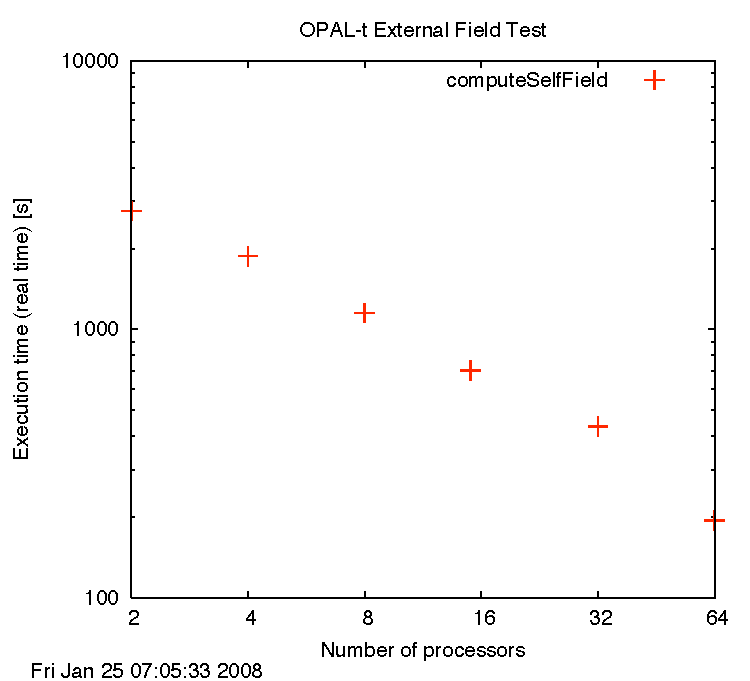
\includegraphics[width=.3\linewidth,angle=0]{figures/computeSelfField}
%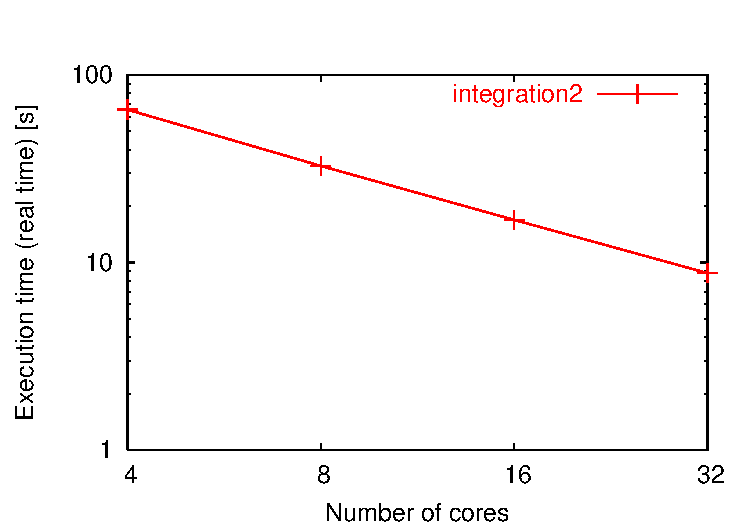
\includegraphics[width=.3\linewidth,angle=0]{figures/integration2}
%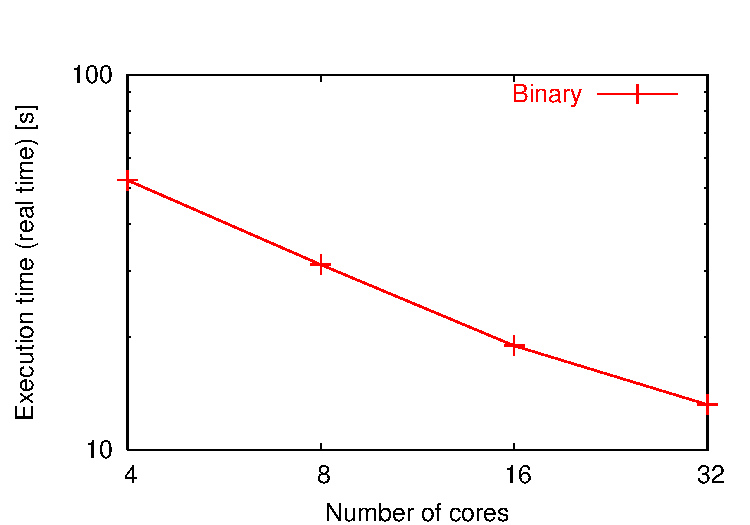
\includegraphics[width=.3\linewidth,angle=0]{figures/Binary}
%\vspace{-5mm}
%\caption{Longitudinal voltage seen by the particle in the middle of the bunch (upper left) and  mean energy gain over the $12 \mbox{mm}$ gap. RMS~$x$ (lower left) and normalised emittance $\epsilon_{xn}$.}
%\label{fig:timings-1}
%\end{center}
%\end{figure}
\clearpage
\section{Discussion}

The \opalt, Astra comparison done in section \ref{sec:OPALAstra} shows ....

With \opalt and IMPACT-T we obtain the same results in context of the pulsed
gun (OBLA) and parts of the following injector structure as shown in section
\ref{sec:OPALImpactt}.

Within the PSI SwissFEL project and our available computing infrastructure a    
factor of $\sim \bf 6$ can be expected w.r.t. Astra, for a comparable but full  
3D simulation, as shown in section \ref{sec:OPALAstra}. We also mention that    
for precise simulations i.e. when a large number of simulation particles must   
be used, parallel tools such as \opal\ or IMPACT-T are mandatory.               


\appendix
\section{Input Files}
The input files, field maps and analysis scripts can be found at 
\url{svn+ssh://savannah01.psi.ch/repos/amas/amas/OPAL/trunk/opal-Doc/Notes/Code-Comparison} in the AMAS repository. As soon as this code comparison project reaches
maturity we will post all data necessary to reproduce the presented results on
the AMAS webpage at \url{http://amas.web.psi.ch/tools/OPAL/index.html}. The test
from appendix \ref{app:extftest} is already part of the daily regression test
suite. The results are online at \url{http://amas.web.psi.ch/regressiontests}.
We plan to have all tests of this report in out daily regression test suite.

Here we only list the input files of the \opal, IMPACT-T tests.

\subsection{Drift Test: {\it opal-drift1.in}}
\begin{verbatim}
Option, TFS=FALSE;
Option, ECHO=FALSE;
Option, PSDUMPFREQ=5;

Title,string="OPAL";

Edes=1.0;
gamma=(Edes+PMASS)/PMASS;
beta=sqrt(1-(1/gamma^2));
gambet=gamma*beta;
P0 = gamma*beta*PMASS;
brho = (PMASS*1.0e9*gambet) / CLIGHT;
value,{gamma,brho,Edes,beta,gambet};

sol0: Solenoid, L=0.12, KS=0.31250, FMAPFN="1T2.T7", ELEMEDGE=0.1;

l1:   Line = (sol0);

Dist1:DISTRIBUTION, DISTRIBUTION=gauss,
sigmax=  1.0e-03, sigmapx=1.0e-4, corrx=0.5,
sigmay=  2.0e-03, sigmapy=1.0e-4, corry=-0.5,
sigmat=  3.0e-03, sigmapt=1.0e-4, corrt=0.0;

Fs1:FIELDSOLVER, FSTYPE=FFT, MX=16, MY=16, MT=128,
                 	PARFFTX=true, PARFFTY=true, PARFFTT=false,
                 	BCFFTX=open, BCFFTY=open, BCFFTT=open,
     		BBOXINCR=1.0, GREENSF=INTEGRATED;

beam1: BEAM, PARTICLE=ELECTRON, pc=P0, NPART=5e4, BFREQ=1498.953425154e6, 
		         BCURRENT=0.032912, CHARGE=-1;

Select, Line=l1;

track,line=l1, beam=beam1, MAXSTEPS=200, DT=1.0e-12;
 run, file = "track_output", turns = 1, method = "PARALLEL-T", 
         beam=beam1, fieldsolver=Fs1, distribution=Dist1;
endtrack;
stop;
\end{verbatim}

\subsection{Gun Test: {\it Gun-test-1.in} {\it Gun-test-2.in}}
The {\it Gun-test-1.in} has no space charge, where {\it Gun-test-2.in} has space
charge enabled. The total charge in {\it Gun-test-2.in} of the beam is $Q=6
~10^{-12}~ \mbox{C}$.

In order to run the simulation without space charge, the FIELDSOLVER attribute
must be set to NONE:
\begin{verbatim}
Fs1:FIELDSOLVER, FSTYPE=NONE, MX=32, MY=32, MT=32, 
                 PARFFTX=true, PARFFTY=true, PARFFTT=false,
                 BCFFTX=open, BCFFTY=open, BCFFTT=open, 
                 BBOXINCR=1, GREENSF=INTEGRATED;
\end{verbatim}
The OPAL input file below we use 39 energy bins.

\begin{verbatim}
Option, TFS=FALSE;
Option, ECHO=FALSE;
Option, PSDUMPFREQ=10;

Title,string="OPAL gun test";

Edes=1.0E-9;
gamma=(Edes+EMASS)/EMASS;
beta=sqrt(1-(1/gamma^2));
gambet=gamma*beta;
P0 = gamma*beta*EMASS;
brho = (EMASS*1.0e9*gambet) / CLIGHT;

value,{gamma,brho,Edes,beta,gambet};

SP1: Solenoid, L=1.20, ELEMEDGE=-0.5265, FMAPFN="1T1.T7", KS=0.11;
SP2: Solenoid, L=1.20, ELEMEDGE=-0.3920, FMAPFN="1T2.T7", KS=0.00000;
SP3: Solenoid, L=1.20, ELEMEDGE=-0.2620, FMAPFN="1T2.T7", KS=0.00000;

gun: RFCavity, L=0.018, VOLT=-131/(1.052*2.658), FMAPFN="1T3.T7", 
                           ELEMEDGE=0.00, TYPE="STANDING", FREQ=1.0e-6;

l1:   Line = (gun,sp1,sp2,sp3); 

qb=6.0e-12;
rf=1498.956e6;
v0=beta*CLIGHT;
T1s = 6.5e-12;
lz  = T1s*v0;
value,{v0,lz};

Dist1:DISTRIBUTION, DISTRIBUTION=gungauss,
sigmax=  0.00030, sigmapx=0.0, corrx=0.0,
sigmay=  0.00030, sigmapy=0.0, corry=0.0,
sigmat=  lz, sigmapt=1.0, corrt=0.0 , TEMISSION=39.0e-12, NBIN=39;

Fs1:FIELDSOLVER, FSTYPE=FFT, MX=32, MY=32, MT=32, 
                 PARFFTX=true, PARFFTY=true, PARFFTT=false,
                 BCFFTX=open, BCFFTY=open, BCFFTT=open, 
                 BBOXINCR=1, GREENSF=INTEGRATED;

beam1: BEAM, PARTICLE=ELECTRON, pc=P0, NPART=5e4, BCURRENT=rf*qb, 
                            BFREQ=rf, CHARGE=-1;

Select, Line=l1;

track,line=l1, beam=beam1, MAXSTEPS=2000, DT=1.0e-13;
 run, file = "track_output", turns = 1, method = "PARALLEL-T", beam=beam1, 
         fieldsolver=Fs1, distribution=Dist1;
endtrack;
Stop;
\end{verbatim}

\subsection{External Field Test: opal-valid.in} \label{app:extftest}

\begin{verbatim}
Option, TFS=FALSE;
Option, ECHO=FALSE;
Option, PSDUMPFREQ=20;

Title,string="OPAL";

Edes=1.0;
gamma=(Edes+PMASS)/PMASS;
beta=sqrt(1-(1/gamma^2));
gambet=gamma*beta;
P0 = gamma*beta*PMASS;
brho = (PMASS*1.0e9*gambet) / CLIGHT;
value,{gamma,brho,Edes,beta,gambet};

sol0: Solenoid, L=0.12, KS=0.31250, FMAPFN="1T2.T7", ELEMEDGE=0.0580;

// add 1.205 m to z_0 to get the peak!!
sol1: Solenoid, L=0.001, KS=0.08300, FMAPFN="1T5.T7", ELEMEDGE=0.364;
sol2: Solenoid, L=0.001, KS=-0.0830, FMAPFN="1T5.T7", ELEMEDGE=0.464;
sol3: Solenoid, L=0.001, KS=0.04780, FMAPFN="1T5.T7", ELEMEDGE=0.864;
sol4: Solenoid, L=0.001, KS=-0.0478, FMAPFN="1T5.T7", ELEMEDGE=0.964;

sol5: Solenoid, L=0.001, KS=0.073250, FMAPFN="1T5.T7", ELEMEDGE=1.364;
sol6: Solenoid, L=0.001, KS=-0.07325, FMAPFN="1T5.T7", ELEMEDGE=1.464;
sol7: Solenoid, L=0.001, KS=0.083470, FMAPFN="1T5.T7", ELEMEDGE=1.864;
sol8: Solenoid, L=0.001, KS=-0.08347, FMAPFN="1T5.T7", ELEMEDGE=1.964;

rf1: RFCavity, L=0.54, VOLT=19.961, FMAPFN="1T3.T7", ELEMEDGE=0.129, 
   		      TYPE="STANDING", FREQ=1498.956, LAG=193.0/360.0;
rf2: RFCavity, L=0.54, VOLT= 6.250, FMAPFN="1T4.T7", ELEMEDGE=0.129, 
                        TYPE="STANDING", FREQ=4497.536, LAG=136.0/360.0;

lrf0: RFCavity, L=0.0253, VOLT=14.750*30/31, FMAPFN="INLB-02-RAC.Ez", 
		       ELEMEDGE=2.73066, TYPE="TRAVELING", NUMCELLS=40, 
		       MODE=1/3, ACCURACY=39, FREQ=1498.956, LAG=248.0/360.0;

l1:   Line = (sol0,rf1,rf2,sol1,sol2,sol3,sol4,sol5,sol6,sol7,sol8,lrf0);

Dist1:DISTRIBUTION, DISTRIBUTION=gauss,
sigmax=  1.0e-03, sigmapx=1.0e-4, corrx=0.5,
sigmay=  2.0e-03, sigmapy=1.0e-4, corry=-0.5,
sigmat=  3.0e-03, sigmapt=1.0e-4, corrt=0.0;

Fs1:FIELDSOLVER, FSTYPE=FFT, MX=16, MY=16, MT=128,
                 PARFFTX=true, PARFFTY=true, PARFFTT=false,
                 BCFFTX=open, BCFFTY=open, BCFFTT=open,
     BBOXINCR=1.0, GREENSF=INTEGRATED;


beam1: BEAM, PARTICLE=ELECTRON, pc=P0, NPART=5e4, BFREQ=1498.953425154e6, 
               BCURRENT=0.032912, CHARGE=-1;

Select, Line=l1;

track,line=l1, beam=beam1, MAXSTEPS=14000, DT=1.0e-12;
 run, file = "track_output", turns = 1, method = "PARALLEL-T", beam=beam1, 
         fieldsolver=Fs1, distribution=Dist1;
endtrack;
Stop;

\end{verbatim}

%\section{Astra Files}






\section{IMPACT-T Input Files}
All input files can be found at {\em merlin00.psi.ch:/scratch0/shared/adelmann}.
Please note that you need to sign a form before using IMPACT-T.

\subsection{Drift Test}
\begin{verbatim}
1 1
1.0e-12 200 1
6 50000 1 0 1 0 0.00
16 16 128 1 0.025 0.025 100.0 10
15 1 3 0 0 0.0
0.75e-4   0.0   0.0   1.  1.  0.0     0.0
0.75e-4   0.0   0.0   1.  1.  0.0     0.0
0.50e-2   0.0   0.0   1.  1.  3.0e-2  2.78322
0.032912 1.0e6 0.511005e+06  -1.0 1498.956e6 0.0
0.12 10 20 3 0.1 0.31250 2.0 0.001 0.0 0.0 0.0 0.0 0.0 /
\end{verbatim}
\subsection{Gun Test}
In order to generate the 39 gun input files, Thomas Schietinger wrote a Python
script (runOBLAWithGun.py). Usage {\it runOBLAWithGun.py SP1B=110 SP4B=50
VGAP=500}.
One of the input files which defines $1/39$ of the total charge is shown bellow: 
\begin{verbatim}
!Welcome to IMPACT-T input file.
!All comment lines start with "!" as the first character of the line.
!
!Purpose: use to track one particle and obtain the static fields 
!         as function of time
!         stored in fort.14
!  ./plotfort.sh 14 "Pulsed Minicoil 4200 [A]   " 1 5 "z [m]" "Bz [Gauss]"
!  ./plotfort.sh 14 "gunb11   " 1 5 "z [m]" "Bz [Gauss]"  
!
!
! processor layout
! col row
1 1 /
!
! information needed by the integrator:
! step-size, number of steps, and number of bunches/bins (??)
!
!   dt    Ntstep  Nbunch
1.0e-13 2000 39 /
!
! more information needed by the integrator:
! phase-space dimension, number of particles, a series of flags
! that set the type of integrator, error study, diagnostics, and
! image charge, and the cutoff distance for the image charge
!
! PSdim  Nptcl   integF  errF  diagF  imchgF  imgCutOff (m)
   6  1282 1 0 1 1 0.02 /
!
! information about mesh: number of points in x, y, and z, type
! of boundary conditions, transverse aperture size (m), 
! and longitudinal domain size (m), which should be larger than the total
! beamline element length
!
!  Nx  Ny  Nz  bcF   Rx    Ry    Lz
32 32 32 1 0.003 0.003 0.05 /
!
!
! distribution type number, restart flag, space-charge substep
! flag, number of emission steps, and max emission time
!
! distType  restartF  substepF  Nemission  Temission
23 0 0 390 3.9e-11 /
!
! the distribution type codes have the following correspondence
!   #  dist type    nparam  parameters (1..21)
!   1  Uniform        21    sigx, sigpx, muxpx, xscale, pxscale, xmu1, xmu2,
!                           sigy, sigpy, muypy, yscale, pyscale, xmu3, xmu4,
!                           sigz, sigpz, muzpz, zscale, pzscale, xmu5, xmu6
!   2  Gauss3         21    as in Uniform
!   3  Waterbag       21    as in Uniform
!   4  Semigauss      21    as in Uniform
!   5  KV3d           21    as in Uniform
!  15  GaussDouble    21    as in Uniform
!  16  read           21    none
!  17  Cylcold        21    as in Uniform
!  18  CylGaussTest   21   
!  19  CylDbGauss     21   
!  20  UniformChain   21   
!
! following three lines contain a total of 21 parameters (seven
! per degree of freedom) particular to the particle distribution
!
! in most cases, the columns are given by
!  sig*   sigp*  mu*p*  *scale  p*scale  xmu*      xmu*
!
0.00030 0.0 0.0 1.0 1.0 0.0 0.0 /
0.00030 0.0 0.0 1.0 1.0 0.0 0.0 /
3.84493391959e-06 0.0 0.0 1.0 1.0 -1.15348017588e-05 0.00197835937429 /
!
! information about the beam: current, kinetic energy, particle
! rest energy, particle charge, scale frequency, and initial
! cavity phase
!
! I/A     Ek/eV     Mc2/eV        Q/e   freq/Hz  phs/rad
0.000230608615385  1.0  0.511005e+06   -1.0    1498.956e6  0.0
! ======= machine description starts here =======
! the following lines, which must each be terminated with a '/',
! describe one beam-line element per line; the basic structure is
! element length, ???, ???, element type, and then a sequence of
! at most 24 numbers describing the element properties
!
! the numeric type codes have the following correspondence
!  #    element    nparams  parameters (v0..v23)
! < 0  bpm           8
!   0  drift tube    2      zedge radius
!   1  quadrupole    9      zedge, quad grad, fileID,
!                             radius, alignment error x, y
!                             rotation error x, y, z
!   2  constFocus    5      zedge, foc grads kx0^2, ky0^2, kz0^2, radius
!   3  solenoid      9      zedge, Bz0, fileID
!                             radius, alignment error x, y
!                             rotation error x, y, z
!   4  dipole       10      zedge, field strength x, y, fileID,
!                             radius, alignment error x, y
!                             rotation error x, y, z
!   5  multipole    10      zedge, typeID (2=sex,3=oct,4=dec),
!                             field strength, fileID,
!                             radius, alignment error x, y
!                             rotation error x, y, z
! 101  DTL          15      zedge, ...
! 102  CCDTL        11      zedge, ...
! 103  CCL          11      zedge, ...
! 104  SC cavity    11      zedge, scale, RF frequency, theta0, fileID,
!                             radius, alignment error x, y
!                             rotation error x, y, z
! 105  SolRF        12      zedge, scale, RF frequency, theta0, fileID,
!                             radius, alignment error x, y
!                             rotation error x, y, z,
!                             Bz0
! 110  EMfld        13      zedge, scale, RF frequency, theta0, fileID,
!                             radius, alignment error x, y
!                             rotation error x, y, z,
!                             field flag (=discrete,=analytic),
!                             coordinate system flag (=cart,=cyl)
! 111  EMfld cart   11      zedge, scale, RF frequency, theta0, fileID,
!                             radius, alignment error x, y
!                             rotation error x, y, z
! 112  EMfld cyl    11      zedge, scale, RF frequency, theta0, fileID,
!                             radius, alignment error x, y
!                             rotation error x, y, z
! 113  EMfld anal   11      zedge, scale, RF frequency, theta0, fileID,
!                             radius, alignment error x, y
!                             rotation error x, y, z
!
! choose 3D solver
0.0 10 20 -5 0.0 0.0 0.0 /
! merge energy  bins into one (btype -7) at z = 1.45 cm:
0.0 1 1    -7 0.0 0.0 0.022 0.0 /
! output particle phase-space and prepare restart file 
!  (btype = -3) at z = 1.50 cm:
!!0.0 1 901  -3 0.0 0.0 1.5E-2  /
! 4mm diode DIODE_4_MM.T7
!0.0060000 10 20 105 0.000 -50.0 1.0E-6 0.0 1.0 0.0253 0.0 0.0 0.0 0.0 0.0 /
!0.0060000 10 20 112 0.000 -124.52 1.0E-6 0.0 3.0 0.0253 0.0 0.0 0.0 0.0 0.0 /
0.018 10 20 112 0.000 -9.988e-05 1.0E-6 0.0 3.0 0.0253 0.0 0.0 0.0 0.0 0.0 /
! start of OBLA beam line (SP1)
0.024 10 20 0 0.0 0.105 /
! SP1: first solenoid, length 1.2 m, starting at z= 6.15-60+gap = -53.85 cm + gap [cm], 
! file ID for field = 1.0 (=> file 1T1.T7), scale factor 1.6 (0.16 T)
1.200 10 20 3 -0.5265 0.00011 1.0 0.005 0.0 0.0 0.0 0.0 0.0 /
1.200 10 20 3 -0.274 0.000000 2.0 0.005 0.0 0.0 0.0 0.0 0.0 /
1.200 10 20 3 -0.054 0.000000 2.0 0.005 0.0 0.0 0.0 0.0 0.0 /
\end{verbatim}

\subsection{External Field Test}
\begin{verbatim}
1 1
1.0e-12 14000 1
6 50000 1 0 1 0 0.00
16 16 128 1 0.025 0.025 100.0 10
15 1 3 0 0 0.0
0.75e-4   0.0   0.0   1.  1.  0.0     0.0
0.75e-4   0.0   0.0   1.  1.  0.0     0.0
0.50e-2   0.0   0.0   1.  1.  3.0e-2  2.78322
0.032912 1.0e6 0.511005e+06  -1.0 1498.956e6 0.0
0.12 10 20 3 0.0580 0.31250 2.0 0.001 0.0 0.0 0.0 0.0 0.0 /
0.540 10 20 112 0.129  20.25 1498.956e6 196.0 3.0 0.108 0.0 0.0 0.0 0.0 0.0 /
0.540 10 20 112 0.129   6.25 4497.536e6 136.0 4.0 0.108 0.0 0.0 0.0 0.0 0.0 /
1.000 10 20 3 0.364  0.08300 5.0 0.001 0.0 0.0 0.0 0.0 0.0 /
1.000 10 20 3 0.464 -0.08300 5.0 0.001 0.0 0.0 0.0 0.0 0.0 /
1.000 10 20 3 0.864  0.04780 5.0 0.001 0.0 0.0 0.0 0.0 0.0 /
1.000 10 20 3 0.964 -0.04780 5.0 0.001 0.0 0.0 0.0 0.0 0.0 /
1.000 10 20 3 1.364  0.07325 5.0 0.001 0.0 0.0 0.0 0.0 0.0 /
1.000 10 20 3 1.464 -0.07325 5.0 0.001 0.0 0.0 0.0 0.0 0.0 /
1.000 10 20 3 1.864  0.08347 5.0 0.001 0.0 0.0 0.0 0.0 0.0 /
1.000 10 20 3 1.964 -0.08347 5.0 0.001 0.0 0.0 0.0 0.0 0.0 /
0.1000000 10 20 105  2.6640000 5.0003e6 1498.956e6 254.0 2 0.0253 0. 0. 0. 0. 0. /
2.6000000 10 20 105  2.7640000 5.7848e6 1498.956e6 285.0 3 0.0253 0. 0. 0. 0. 0. /
2.6000000 10 20 105  2.7640000 5.7848e6 1498.956e6 345.0 4 0.0253 0. 0. 0. 0. 0. /
0.1000000 10 20 105  5.3640000 5.0003e6 1498.956e6 254.0 5 0.0253 0. 0. 0. 0. 0. /
\end{verbatim}

\section{Implementation of the Thermal Emittance and the Emission Model} \label{app:emission}
The thermal (or initial) emittance of an electron bunch emitted from a cathode
by photo effect represents the lowest normalized emittance of a photo injector.
A correct description of this intrinsic emittance is thus essential to properly
evaluate the possible (theoretical) performance of photo injector based
accelerators. \\
An algorithm for generating thermal emittance in the emission process was
implemented into the \opalt \cite{OPAL} tracking code.
In a first step, and in order to compare with ASTRA \cite{ASTRA} simulations, a
simple model as described in \cite{KLAUS} was used. This model is basically
describing the thermal emittance of semiconductors like $\rm{Cs_2 Te}$ but
neglects the energy distribution in metals like $\rm{Cu}$. Therefore, in a
second step, the model was extended to properly describe the thermal emittance
in metals. A detailed theoretical description of the subject is given in
\cite{DAVE}.\\

\subsection{Basic theory}
The thermal emittance calculation is described by the probability
$P(E_f,E_{ph})$ for a photon of energy $E_{ph}=\hbar\omega$ exciting an electron
to a final state energy $E_f$: $$P(E_f,E_{ph}) \propto N_f(E_f) N_i(E_i)$$ with
$N_f(E_f)$ being the density of final state and $N_i(E_i = E_f - E_{ph})$ the
density of initial state \cite{KLAUS}. The thermal emittance can then be
computed to be \cite{DAVE} $$\epsilon_{th} = \sigma_{rms} \cdot \sqrt{\frac{2
E_{kin}^{ave}}{3 m_0 c^2}} .$$ When assuming a uniform radial distribution of
radius $r$, $\sigma_{rms} = \frac{r}{2}$.\\
The emission of electrons can be described by the three-step model. In the first
step, an electron from the valence band is excited to the conduction band by
absorption of a photon. Due to the energy gap between valence band and
conduction band, photon energy must be larger than the gap. The second step  the
involves the transport of the electron to the surface and includes effects like
scattering. In the last step, the electron overcomes the potential barrier at
the surface and is emitted into the vacuum.

\subsubsection{A simple model for semiconductors: the case of $\rm{Cs_2Te}$}
In the simple model described in \cite{KLAUS}, electrons from the valence band
are excited to the first conduction band maximum at $E_f =$ \unit{4.05}{eV} for
the used laser (photon) energies. The electrons are then emitted isotropically
into the half-sphere over the cathode (already behind the surface potential
barrier) with an average kinetic energy of $$E_{kin}^{ave} = E_f - (E_G + E_A) =
0.55 \, \rm{eV}$$ for a band gap of $E_G =$ \unit{3.3}{eV} and an electron
affinity of $E_A =$ \unit{0.2}{eV}. The obtained thermal emittance values can be
considered as an upper limit only (for details refer to \cite{KLAUS}).

\subsubsection{The simple model: comparison OPAL / ASTRA}
The simple model was implemented in OPAL to compare the results with ASTRA. As
in the ASTRA generator settings, we assume uniform transverse distributions $x$,
in $y$, $p_x$, $p_y$, as well as an isotropic distribution in $p_z$. The
longitudinal distribution ($z$, or better: $t$) in this special case was chosen
to be Gaussian. \\
In order to properly model the photo emission process, the OPAL emission was
changed from a $z$-based procedure to a time step based one. That means, the
initial time distribution of the photo cathode laser is sampled into a specified
number of time bins and the content of each time bin (i.e. the number of photo
electrons to be emitted in this time interval) is then emitted from the photo
cathode at $z$=0 according to the time steps of the simulation.\\
Figure \ref{PLOT1} shows distribution functions of the relevant parameter
distributions for both programs at the generator level. A good agreement was
found.

\begin{figure}[ht!]
    \begin{center}
%    \epsfig{file=pictures/vergleich1.eps,angle=270.,width=13cm}
    \end{center}
    \caption{\small \sl To be updated.} 
    \label{PLOT1}
\end{figure}

\subsubsection{The advanced model for metals}
In metals, electrons populating the valence band between $E_{min}=0$ up to the
Fermi energy $E_{max}=E_F$ are transferred to the band of excited states by
absorption of a photon of energy $E_{ph}$ above the energy gap described by the
material's work function $\Phi$ which, in the presence of an external electric
field $E_{ext}$, is reduced to an effective work function $\Phi_{eff}$ by the
Schottky effect. The reduction amounts to
%
$$\Delta = e \sqrt{e E_{ext} / 4 \pi \epsilon_0}$$
%
and thus $E_{ph} \geq \Phi_{eff} = \Phi - \Delta$. Hence, electrons with initial
energies $E_i \in [E_F + \Phi_{eff} - E_{ph}, E_F]$ are excited to a final state
with $E_f \in [E_F + \Phi_{eff}, E_F + E_{ph}]$. \\
Emission into vacuum over the potential barrier $E_F + \Phi_{eff}$ leads to a
kinetic energy of the emitted electrons in the vacuum of 
%
$$E_{kin} = E_i + E_{ph} - (E_F + \Phi_{eff})$$
%
in the interval $E_{kin} \in [0,E_{ph} - \Phi_{eff}]$. The average kinetic
energy assuming a uniform distribution of $E_i$ (as shown in \cite{ANGHEL}) is
thus
%
$$E_{kin}^{ave} = \frac{1}{2} E_{kin}^{max} = \frac{E_{ph} - \Phi_{eff}}{2} .$$
%
The model can be further refined by assuming a Fermi-Dirac distribution for the
initial energy $E_i$ of the electrons, as described in \cite{DAVE}: $$N_i(E_i) =
\frac{1}{1 + e^{\frac{E_i - E_F}{k_B T}}}$$ which, compared to the assumption of
a uniform energy distribution of $E_i$, leads essentially only to a smearing of
(the higher) initial electron energies $E_i$ around $E_F$.\\
Electrons with an internal emission angle $\varphi > \varphi_{max}$ (relative
to the surface normal) will however not be able to pass the surface potential
barrier since their longitudinal momentum is too small. The escape criterion is
therefore defined by limiting $\varphi$ according to 
%
$$\varphi_{max} (E_i) = \arccos \sqrt{\frac{E_F +\Phi_{eff}}{E_i + E_{ph}}} .$$
%
Thus, electrons with an internal emission angle $\varphi = \varphi_{max}$ will
be emitted with an external angle of $\varphi ' = \frac{\pi}{2}$. Conservation
of the transverse momenta $p_x = p \cdot \sin \varphi \cos \theta = p_x '$ and
$p_y = p \cdot \cos \varphi \sin \theta = p_y '$ allows to correlate the
internal angular distribution to the external one via 
%
$$\frac{\sin\varphi '}{\sin \varphi} = \sqrt{\frac{E_i + E_{ph}}{E_i + E_{ph} - (E_F + \Phi_{eff})}} ,$$
%
where $\varphi \in [0, \varphi_{max}]$ and $\theta \in [0, \pi]$. 
$p$ is determined by the relation
%
$$p= m_0 c \sqrt{\gamma^2 - 1} = m_0 c\sqrt{\frac{2 E_{kin}^{ave}}{m_0 c^2}} .$$ 


\begin{thebibliography}{9}
\bibitem{OPAL} The OPAL (Object Oriented Parallel Accelerator Library) Framework, PSI-PR-08-02, \url{http://amas.web.psi.ch/tools/OPAL/index.html}, 2008-2010
\bibitem{ASTRA} ASTRA by K.Fl\"ottmann,  \url{http://www.desy.de/~mpyflo/}
\bibitem{KLAUS} K. Fl\"ottmann, Note on the thermal emittance of electrons emitted by Cesium Telluride photo cathodes, TESLA-FEL 97-01.
\bibitem{DAVE} D. Dowell et all., SLAC-PUB-13535, Phys. Rev. ST Accel. Beams {\bf (12)} 7, doi:10.1103/PhysRevSTAB.12.074201
\bibitem{ANGHEL} A.Anghel, presentation at the FELSI meeting, 3.2.2009.
\bibitem{PhysRevSTAB.13.064201} Yang, J. J et.al, Beam dynamics in high intensity cyclotrons including neighboring bunch effects: Model, implementation, and application, Phys. Rev. ST Accel. Beams, {\bf (13)} 6, DOI:10.1103/PhysRevSTAB.13.064201, 2010
\bibitem{Adelmann20104554} A. Adelmann et.al, A fast parallel Poisson solver on irregular domains applied to beam dynamics simulations, Journal of Computational Physics, {\bf (229)} 12, DOI: 10.1016/j.jcp.2010.02.022, 2010
\bibitem{CTF3Gun} L. Rinolfi et.al, CTF3 3 GHz RF gun test at CERN, \url{http://irfu.cea.fr/Phocea/file.php?class=std&&file=Doc/Care/care-report-08-044.pdf}, 2008
\end{thebibliography}


\end{document}                        % End of document
 
